

% ----------------------------------------------------------------------
%                   LATEX TEMPLATE FOR PhD THESIS
% ----------------------------------------------------------------------

% based on Harish Bhanderi's PhD/MPhil template, then Uni Cambridge
% http://www-h.eng.cam.ac.uk/help/tpl/textprocessing/ThesisStyle/
% corrected and extended in 2007 by Jakob Suckale, then MPI-CBG PhD programme
% and made available through OpenWetWare.org - the free biology wiki


%: Style file for Latex
% Most style definitions are in the external file PhDthesisPSnPDF.
% In this template package, it can be found in ./Latex/Classes/
\documentclass[twoside, 12pt]{thesis}


%: Macro file for Latex
% Macros help you summarise frequently repeated Latex commands.
% Here, they are placed in an external file /Latex/Macros/MacroFile1.tex
% An macro that you may use frequently is the figuremacro (see introduction.tex)
\newcommand{\comment}[1]{}
\newcommand{\myparagraph}[1]{\paragraph{#1}\mbox{}\\}
\newcommand{\pw}[4]{
	\begin{cases}\displaystyle
		#1 & \mbox{#2},\\ 
		#3 & \mbox{#4}
	\end{cases}
}

\newcommand{\cref}[1]{Chap.~\ref{#1}}
\newcommand{\Cref}[1]{Chapter~\ref{#1}}
\newcommand{\sref}[1]{Sec.~\ref{#1}}
\newcommand{\Sref}[1]{Section~\ref{#1}}
\newcommand{\aref}[1]{App.~\ref{#1}}
\newcommand{\Aref}[1]{Appendix~\ref{#1}}
\newcommand{\fref}[1]{Fig.~\ref{#1}}
\newcommand{\Fref}[1]{Figure~\ref{#1}}
\newcommand{\tref}[1]{Tab.~\ref{#1}}
\newcommand{\Tref}[1]{Table~\ref{#1}}
\newcommand{\pgref}[1]{p.~\pageref{#1}}
\newcommand{\Pgref}[1]{page~\pageref{#1}}



\def\eqrefs#1#2{(\protect\ref{#1}--\protect\ref{#2})}

\newcommand{\alert}[1]{\textcolor{red}{#1}}
\newcommand{\PN}[1][N]{\ensuremath{\text{P}_{#1}}}
\newcommand{\MCPN}[1][N]{\ensuremath{\text{MCP}_{#1}}}
\newcommand{\SN}[1][N]{\ensuremath{\text{S}_{#1}}}
\newcommand{\SPN}[1][N]{\ensuremath{\text{SP}_{#1}}}
\newcommand{\Oh}{\ensuremath{\mathcal{O}}}

\newcommand{\R}[1][]{\mathbb{R}^{#1}}
\newcommand{\mat}[1]{\mathbf{#1}}
\newcommand{\src}{q}

\newcommand{\sla}{\ensuremath{\shortleftarrow}}
\newcommand{\sra}{\ensuremath{\shortrightarrow}}

\newcommand{\br}{\ensuremath{\mathbf{r}}}
\newcommand{\bv}{\ensuremath{\mathbf{v}}}
\newcommand{\bn}{\ensuremath{\mathbf{n}}}
\newcommand{\be}{\ensuremath{\mathbf{e}}}
\newcommand{\bJ}{\ensuremath{\mathbf{J}}}

\newcommand{\bomega}{\mathbf{\Omega}}
\newcommand{\Sphere}{\ensuremath{S_2}}
\newcommand{\Emin}{\ensuremath{E_{\text{min}}}}
\newcommand{\Emax}{\ensuremath{E_{\text{max}}}}

\newcommand{\der}[3][]{\ensuremath{\frac{\text{d}^{#1}{#2}}{\text{d} {#3}^{#1}}}}
\newcommand{\pd}[3][]{\ensuremath{\frac{\partial^{#1}#2}{\partial #3^{#1}}}}
\newcommand{\grad}{\nabla}
\newcommand{\gradcomp}[1]{\nabla_{\!#1}}
\newcommand{\lapv}{\nabla^2}
\newcommand{\lap}{\nabla^2}

\renewcommand{\d}[1]{\ensuremath{\text{d}#1\,}}
\newcommand{\intE}[4][]{\int_{#2}^{#3}#4\,\d{E#1}}
\newcommand{\intEg}[3]{\int_{E^{#1}}^{E^{#2}}#3\,\d{E}}
\newcommand{\intA}[2][]{\int_{\Sphere}#2\,\d{\bomega#1}}
\newcommand{\intX}[2][X]{\int_{#1}#2\,\d{x}}

\newcommand{\sumg}{\sum_{{g'\neq g}}}
\newcommand{\summ}[2]{\sum_{#1}^{#2}}
\newcommand{\suma}[3][l]{\summ{#1=#2}{#3}}

\newcommand{\abs}[1]{\ensuremath{\left\vert#1\right\vert}}
\newcommand{\norm}[2][]{\ensuremath{\lVert#2\rVert_{#1}}}

\newcommand{\pX}[1][]{\partial X^{#1}}
\newcommand{\pV}[1][]{\partial V}
\newcommand{\VV}{V}

\newcommand{\polar}{\vartheta}
\newcommand{\azimuthal}{\varphi}
\newcommand{\sint}{\sin \polar}
\newcommand{\sinp}{\sin \azimuthal}
\newcommand{\cost}{\cos \polar}
\newcommand{\cosp}{\cos \azimuthal}
\newcommand{\db}{\ensuremath{\d\xi}}

\newcommand{\Lp}[1][p]{L^{#1}}
\newcommand{\Hp}[1][p]{H^{#1}}
\newcommand{\Id}{\ensuremath{I}}
\newcommand{\Dom}[1]{\mathcal{D}(#1)}

\newcommand{\Y}[2]{Y_{#1}^{#2}}
\renewcommand{\P}[2]{P_{#1}^{#2}}
\newcommand{\YY}[1][n]{\mathbf{Y}_{#1}}
\newcommand{\Yc}[2]{\bar{Y}_{#1}^{#2}}
\newcommand{\YYc}[1][n]{\bar{\mathbf{Y}}_{#1}}

\newcommand{\PP}[1][n]{\mathbb{P}^{(#1)}}
\newcommand{\PPP}[2][n]{P^{(#1)}_{#2}}
\renewcommand{\AA}[1][n]{\mathbb{A}^{(#1)}}
\newcommand{\AAA}[2][n]{A^{(#1)}_{#2}}
\newcommand{\BB}[1][n]{\mathbb{B}^{(#1)}}
\newcommand{\BBB}[2][n]{B^{(#1)}_{#2}}
\newcommand{\CC}[1][n]{\mathbb{C}^{(#1)}}
\newcommand{\CCC}[2][n]{C^{(#1)}_{#2}}


\newcommand{\kron}[2]{\delta_{#1#2}}
\newcommand{\Sym}[1]{\left[#1\right]_{\mbox{\scriptsize sym}}}
\newcommand{\eye}{\mathbb{I}}
\newcommand{\detr}[1][n]{\mathscr{D}_{#1}}
\newcommand{\contr}[1][n]{\cdot}%\underset{#1}{\cdot}}
\newcommand{\perm}[1]{\pi(#1)}

\newcommand{\angmom}[2]{\ensuremath{\phi_{#1}^{#2}}}
\newcommand{\fmom}[1][n]{\Phi_{#1}}
\newcommand{\qmom}[1][n]{Q_{#1}}
\newcommand{\Sa}[2][]{\Sigma^{#1}_{#2}}
\newcommand{\mst}{\underline{\sigma_t}}
%\newcommand{\Sym}[2]{\mathscr{S}^{(#1)}\left[#2\right]}

\newcommand{\angflux}{\ensuremath{\psi}}

\DeclareMathOperator{\sgn}{sgn}
\DeclareMathOperator{\esssup}{ess\,sup\,}
\DeclareMathOperator{\argmin}{argmin\,}
\DeclareMathOperator{\diag}{diag\,}
\DeclareMathOperator{\col}{col\,}
\DeclareMathOperator{\trace}{tr\,}

\usepackage{colortbl}
\newlength\celldim \newlength\fontheight \newlength\extraheight
\setlength\celldim{2em}
\settoheight\fontheight{A}
\setlength\extraheight{\celldim - \fontheight}

\newcolumntype{A}{ >{\centering } p{1em}  <{\rule[-.5\extraheight]{0pt}{\extraheight+\fontheight}}}
\newcolumntype{B}{ >{\centering } p{11em}  <{\rule[-.5\extraheight]{0pt}{\extraheight+\fontheight}}}
\newcolumntype{C}{ >{\centering } p{11em} <{\rule[-.5\extraheight]{0pt}{\extraheight+\fontheight}}}
\newcolumntype{D}{ >{\centering } p{4em}  <{\rule[-.5\extraheight]{0pt}{\extraheight+\fontheight}}}
\newcommand{\nl}{\tabularnewline\hline}




%: ----------------------------------------------------------------------
%:                  TITLE PAGE: name, degree,..
% ----------------------------------------------------------------------
% below is to generate the title page with crest and author name

\title{Mathematical Modeling of Neutron Transport}



% ----------------------------------------------------------------------
% The section below defines www links/email for author and institutions
% They will appear on the title page of the PDF and can be clicked
\ifpdf
  \author{\href{mailto:mhanus@kma.zcu.cz}{Ing. Milan Hanu{\v s}}}
%  \cityofbirth{born in XYZ} % uncomment this if your university requires this
%  % If city of birth is required, also uncomment 2 sections in PhDthesisPSnPDF 
%  % Just search for the "city" and you'll find them.
  \collegeordept{\href{http://www.kma.zcu.cz}{Department of Mathematics}}
  \university{\href{http://www.zcu.cz}{University of West Bohemia, Pilsen}}

  % The crest is a graphics file of the logo of your research institution.
  % Place it in ./0_frontmatter/figures and specify the width 
  \crest{\includegraphics[width=10cm]{fav_en_cmyk}}
  
% If you are not creating a PDF then use the following. The default is PDF.
\else
  \author{Ing. Milan Hanu{\v s}}
  \collegeordept{Department of Mathematics} 
  \university{University of West Bohemia, Pilsen}
  \crest{\includegraphics[width=10cm]{fav_en_cmyk}}
\fi

\renewcommand{\submittedtext}{Thesis Submitted in Partial Fulfillment of the Requirements for the Degree: \textit{Doctor
of Philosophy (Ph.D.)}}
\supervisor{Doc. Ing. Marek Brandner, Ph.D.}
\degree{Doctor of Philosophy (Ph.D.)}
\degreedate{November 2014}


% ----------------------------------------------------------------------
       
% turn of those nasty overfull and underfull hboxes
\hbadness=10000
\hfuzz=50pt

 
%: --------------------------------------------------------------
%:                  FRONT MATTER: dedications, abstract,..
% --------------------------------------------------------------

\begin{document}

%\language{english}

% sets line spacing
\renewcommand\baselinestretch{1.2}
\baselineskip=18pt plus1pt


%: ----------------------- generate cover page ------------------------

 

% command to print the title page with above variables
\maketitle

%: ----------------------- cover page back side ------------------------
% Your research institution may require reviewer names, etc.
% This cover back side is required by Dresden Med Fac; uncomment if needed.

%\newpage
%\vspace{10mm}
%1. Reviewer: Name

%\vspace{10mm}
%2. Reviewer: 

%\vspace{20mm}
%Day of the defense:

%\vspace{20mm}
%\hspace{70mm}Signature from head of PhD committee:



%: ----------------------- abstract ------------------------

% Your institution may have specific regulations if you need an abstract and where it is to be placed in the document. The default here is just after title.

%
% Thesis Abstract -----------------------------------------------------

\begin{alwayssingle} \pagestyle{empty}
  \begin{center}
  \vspace*{1.5cm}
  {\Large \bfseries  Abstract}
  \end{center}
  \vspace{0.5cm}
\begin{quote}

The subject of this work is computational modeling of neutron transport relevant to economical and safe operation of
nuclear facilities. The general mathematical model of neutron transport is provided by the linear Boltzmann's transport
equation\comment{This first-order partial differential equation with integral terms describes the dependence of neutron
field on six phase-space variables (position, direction, energy)} and the thesis begins with its precise mathematical
formulation and presentation of known conditions for its well-posedness.

\comment{High-dimensionality and complicated structure of the equation for real-world problems preclude analytical
solution and present serious difficulties when a computational solution is attempted. Several dimension-reduction
techniques thus need to be employed along with appropriate numerical solution schemes. This is the subject of the}
In the following part, we study approximation methods for the transport equation, starting with the classical
discretization of energetic dependence and followed by the review of two most widely used methods for approximating 
directional dependence (the $\SN$ and $\PN$ methods). While these methods are usually presented independently of each 
other, we show that they can be put into a single framework of Hilbert space projection techniques. This fact is then
used in conjunction with the results of the first part to rigorously prove rotational invariance of the $\PN$
equations and to analyze convergence of the basic iterative scheme for solving the $\SN$ equations. This part of the
thesis is concluded by the description of a finite element method for the final discretization of spatial dependence and a discussion of the solution of the resulting system of
algebraic equations.

The main new results are contained in the following two chapters focusing on the simplified $\PN$ approximation, which
is a computationally more convenient albeit not as mathematically well-founded variant of the $\PN$ approximation. We
prove well-posedness of the weak form of the $\SPN[3-7]$ equations and present a new way of deriving the equations from
an alternative set to the $\PN$ equations, obtained from special linear combination of
spherical harmonics.% (the so-called Maxwell-Cartesian spherical harmonics, hence the abbreviation $\MCPN$ for this
% approximation), u%tilizing its tensor structure. Algebraic manipulations allowing to obtain the $\SPN[3]$-equivalent equations from the
%$\MCPN[3]$ set in an interior of a homogeneous region are explicitly given in \sref{sec:mcp3_red}.

The final part of the thesis contains numerical examples of the $\SN$ and $hp$-adaptive $\SPN$ calculations using a
neutronics framework that has been implemented by the author to the $hp$-adaptive finite element library Hermes2D. The $\SPN[1]$
(or diffusion) model also serves as a basis of a real-world reactor calculation suite co-developed by the author for the
purposes of ``Project TA01020352 -- Increasing utilization of nuclear fuel through optimization of an inner fuel cycle and
calculation of neutron-physics characteristics of nuclear reactor cores''. An example benchmark used to test the code
concludes the thesis.
 

\vspace*{1cm}
%\begin{quote}
{\large \bfseries  Keywords:}

The neutron diffusion approximation, whereby the NTE is reduced to a second-order elliptic PDE (or, when energy
dependence is taken into account implicitly, a weakly coupled non-symmetric system of second-order PDEs with
positive-definite symmetric part -- the so-called \textit{multigroup neutron diffusion approximation}), also forms the

\end{quote}

\clearpage
\selectlanguage{czech}
  \begin{center}
  \vspace*{1.5cm}
  {\Large \bfseries  Abstrakt}
  \end{center}
  \vspace{0.5cm}
\begin{quote}

Práce se zabývá matematickým a numerickým modelováním transportu neutronů, se zaměřením na výpočty neutronových
charakteristik jaderných reaktorů. Obecný matematický model transportu neutronů je reprezentován lineární Boltzmannovou
transportní rovnicí. Práce začíná její přesnou matematickou formulaci a přehledem\linebreak výsledků týkajících se její
řešitelnosti ve druhé kapitole. Následující kapitoly jsou zaměřeny na přibližné metody řešení této rovnice.

Po stručném popisu klasické diskretizace energetické závislosti je hlavní část třetí kapitoly věnována aproximaci
směrové závislosti pomocí dvou stěžejních metod -- metody diskrétních ordinát ($\SN$) a metody sférických harmonických
funkcí ($\PN$). Zatímco obvykle jsou tyto metody formulovány nezávisle, v práci je ukázáno, jak je lze obě popsat pomocí
jednotného rámce jako projekci na podprostor Hilbertova prostoru funkcí definovaných na sféře. Této skutečnosti je
posléze využito při důkazu rotační invariantnosti $\PN$ rovnic a při konvergenční analýze základní iterační
metody pro řešení $\SN$ soustavy.
Třetí kapitola je zakončena popisem aplikace metody konečných prvků na finální diskretizaci prostorové závislosti.

Hlavní nové výsledky této práce se týkají metody zjednodušených sférických harmonických funkcí ($\SPN$), jež představuje
výpočetně efektivní aproximaci metody $\PN$. Ve čtvrté kapitole je standardním \linebreak způsobem odvozena slabá
formulace $\SPN$ rovnic a dokázána její korektnost pro $N = 3,5,7$. V páté kapitole je pak odvozena
nová soustava parciálních diferenciálních rovnic odpovídající $\PN$ aproximaci ($\MCPN$ aproximace). Na příkladu $\MCPN[3]$ aproximace je ukázáno, jak lze využít
tenzorovou strukturu těchto rovnic k transformaci na soustavu ekvivalentní s $\SPN[3]$ aproximací.

V šesté kapitole je popsána implementace $\SN$ a $\SPN$ aproximací do knihovny Hermes2D a na několika
příkladech ukázány základní vlastnosti těchto aproximací.  Speciální pozornost je věnována implementaci nespojité
Galerkinovy metody (pro $\SN$ aproximaci)%, umožňující využít speciální způsob asemblace soustav PDR v knihovně
% Hermes2D, v níž je každá neznámá funkce aproximována na vlastním konečně-prvkovém prostoru. 
a modifikaci standardního indikátoru chyby pro
$hp$-adaptivitu v Hermes2D pro $\SPN$ aproximaci. Práce je ukončena ukázkou řešení standardního 3D benchmarku pomocí
mnohagrupového difúzního kódu, který autor na základě zkušeností s vývojem neutronických modulů v knihovně Hermes2D
vyvinul pro účely projektu ``TA01020352 -- Zvýšení využití jaderného paliva pomocí optimalizace vnitřního palivového
cyklu a výpočtu neutronově-fyzikálních charakt. aktivních zón jaderných reaktorů''.



  \vspace*{1cm}
{\large \bfseries  Klíčová slova:}

%\begin{quote}

The neutron diffusion approximation, whereby the NTE is reduced to a second-order elliptic PDE (or, when energy
dependence is taken into account implicitly, a weakly coupled non-symmetric system of second-order PDEs with
positive-definite symmetric part -- the so-called \textit{multigroup neutron diffusion approximation}), also forms the


\end{quote}

\end{alwayssingle}\selectlanguage{english}


% ---------------------------------------------------------------------- 


% The original template provides and abstractseparate environment, if your institution requires them to be separate. I think it's easier to print the abstract from the complete thesis by restricting printing to the relevant page.
% \begin{abstractseparate}
%   
% Thesis Abstract -----------------------------------------------------

\begin{alwayssingle} \pagestyle{empty}
  \begin{center}
  \vspace*{1.5cm}
  {\Large \bfseries  Abstract}
  \end{center}
  \vspace{0.5cm}
\begin{quote}

The subject of this work is computational modeling of neutron transport relevant to economical and safe operation of
nuclear facilities. The general mathematical model of neutron transport is provided by the linear Boltzmann's transport
equation\comment{This first-order partial differential equation with integral terms describes the dependence of neutron
field on six phase-space variables (position, direction, energy)} and the thesis begins with its precise mathematical
formulation and presentation of known conditions for its well-posedness.

\comment{High-dimensionality and complicated structure of the equation for real-world problems preclude analytical
solution and present serious difficulties when a computational solution is attempted. Several dimension-reduction
techniques thus need to be employed along with appropriate numerical solution schemes. This is the subject of the}
In the following part, we study approximation methods for the transport equation, starting with the classical
discretization of energetic dependence and followed by the review of two most widely used methods for approximating 
directional dependence (the $\SN$ and $\PN$ methods). While these methods are usually presented independently of each 
other, we show that they can be put into a single framework of Hilbert space projection techniques. This fact is then
used in conjunction with the results of the first part to rigorously prove rotational invariance of the $\PN$
equations and to analyze convergence of the basic iterative scheme for solving the $\SN$ equations. This part of the
thesis is concluded by the description of a finite element method for the final discretization of spatial dependence and a discussion of the solution of the resulting system of
algebraic equations.

The main new results are contained in the following two chapters focusing on the simplified $\PN$ approximation, which
is a computationally more convenient albeit not as mathematically well-founded variant of the $\PN$ approximation. We
prove well-posedness of the weak form of the $\SPN[3-7]$ equations and present a new way of deriving the equations from
an alternative set to the $\PN$ equations, obtained from special linear combination of
spherical harmonics.% (the so-called Maxwell-Cartesian spherical harmonics, hence the abbreviation $\MCPN$ for this
% approximation), u%tilizing its tensor structure. Algebraic manipulations allowing to obtain the $\SPN[3]$-equivalent equations from the
%$\MCPN[3]$ set in an interior of a homogeneous region are explicitly given in \sref{sec:mcp3_red}.

The final part of the thesis contains numerical examples of the $\SN$ and $hp$-adaptive $\SPN$ calculations using a
neutronics framework that has been implemented by the author to the $hp$-adaptive finite element library Hermes2D. The $\SPN[1]$
(or diffusion) model also serves as a basis of a real-world reactor calculation suite co-developed by the author for the
purposes of ``Project TA01020352 -- Increasing utilization of nuclear fuel through optimization of an inner fuel cycle and
calculation of neutron-physics characteristics of nuclear reactor cores''. An example benchmark used to test the code
concludes the thesis.
 

\vspace*{1cm}
%\begin{quote}
{\large \bfseries  Keywords:}

The neutron diffusion approximation, whereby the NTE is reduced to a second-order elliptic PDE (or, when energy
dependence is taken into account implicitly, a weakly coupled non-symmetric system of second-order PDEs with
positive-definite symmetric part -- the so-called \textit{multigroup neutron diffusion approximation}), also forms the

\end{quote}

\clearpage
\selectlanguage{czech}
  \begin{center}
  \vspace*{1.5cm}
  {\Large \bfseries  Abstrakt}
  \end{center}
  \vspace{0.5cm}
\begin{quote}

Práce se zabývá matematickým a numerickým modelováním transportu neutronů, se zaměřením na výpočty neutronových
charakteristik jaderných reaktorů. Obecný matematický model transportu neutronů je reprezentován lineární Boltzmannovou
transportní rovnicí. Práce začíná její přesnou matematickou formulaci a přehledem\linebreak výsledků týkajících se její
řešitelnosti ve druhé kapitole. Následující kapitoly jsou zaměřeny na přibližné metody řešení této rovnice.

Po stručném popisu klasické diskretizace energetické závislosti je hlavní část třetí kapitoly věnována aproximaci
směrové závislosti pomocí dvou stěžejních metod -- metody diskrétních ordinát ($\SN$) a metody sférických harmonických
funkcí ($\PN$). Zatímco obvykle jsou tyto metody formulovány nezávisle, v práci je ukázáno, jak je lze obě popsat pomocí
jednotného rámce jako projekci na podprostor Hilbertova prostoru funkcí definovaných na sféře. Této skutečnosti je
posléze využito při důkazu rotační invariantnosti $\PN$ rovnic a při konvergenční analýze základní iterační
metody pro řešení $\SN$ soustavy.
Třetí kapitola je zakončena popisem aplikace metody konečných prvků na finální diskretizaci prostorové závislosti.

Hlavní nové výsledky této práce se týkají metody zjednodušených sférických harmonických funkcí ($\SPN$), jež představuje
výpočetně efektivní aproximaci metody $\PN$. Ve čtvrté kapitole je standardním \linebreak způsobem odvozena slabá
formulace $\SPN$ rovnic a dokázána její korektnost pro $N = 3,5,7$. V páté kapitole je pak odvozena
nová soustava parciálních diferenciálních rovnic odpovídající $\PN$ aproximaci ($\MCPN$ aproximace). Na příkladu $\MCPN[3]$ aproximace je ukázáno, jak lze využít
tenzorovou strukturu těchto rovnic k transformaci na soustavu ekvivalentní s $\SPN[3]$ aproximací.

V šesté kapitole je popsána implementace $\SN$ a $\SPN$ aproximací do knihovny Hermes2D a na několika
příkladech ukázány základní vlastnosti těchto aproximací.  Speciální pozornost je věnována implementaci nespojité
Galerkinovy metody (pro $\SN$ aproximaci)%, umožňující využít speciální způsob asemblace soustav PDR v knihovně
% Hermes2D, v níž je každá neznámá funkce aproximována na vlastním konečně-prvkovém prostoru. 
a modifikaci standardního indikátoru chyby pro
$hp$-adaptivitu v Hermes2D pro $\SPN$ aproximaci. Práce je ukončena ukázkou řešení standardního 3D benchmarku pomocí
mnohagrupového difúzního kódu, který autor na základě zkušeností s vývojem neutronických modulů v knihovně Hermes2D
vyvinul pro účely projektu ``TA01020352 -- Zvýšení využití jaderného paliva pomocí optimalizace vnitřního palivového
cyklu a výpočtu neutronově-fyzikálních charakt. aktivních zón jaderných reaktorů''.



  \vspace*{1cm}
{\large \bfseries  Klíčová slova:}

%\begin{quote}

The neutron diffusion approximation, whereby the NTE is reduced to a second-order elliptic PDE (or, when energy
dependence is taken into account implicitly, a weakly coupled non-symmetric system of second-order PDEs with
positive-definite symmetric part -- the so-called \textit{multigroup neutron diffusion approximation}), also forms the


\end{quote}

\end{alwayssingle}\selectlanguage{english}


% ---------------------------------------------------------------------- 

% \end{abstractseparate}


%: ----------------------- tie in front matter ------------------------ 

\frontmatter
% Thesis Acknowledgements ------------------------------------------------


%\begin{acknowledgementslong} %uncommenting this line, gives a different acknowledgements heading
\begin{acknowledgements}      %this creates the heading for the acknowlegments

I would like to thank my supervisor Marek Brandner, for all his support and guidance throughout the course of 
my Ph.D. studies. My thanks also belong to all members of our TACR-PAMG team, especially to the ``Himalaya
Expedition group'' Roman, Hanka and Zby{\v n}{\' a}k, who influenced my thinking in so many ways both direct and
indirect. In particular, I would like to thank Roman for explaining to me many of his great ideas (not only about
homebrewing). Having said so, I cannot fail to mention how Hanka took care of us when we were so deeply immersed in discussing those ideas, for which I (and Roman certainly too)
am so grateful.

I would also like to thank all the great people whom I had an honor to work with during my Ph.D. studies and were
not mentioned above. Namely to Luk{\' a}{\v s} Korous, with whom I spent so many productive days working on Hermes,
Pavel {\v S}ol{\' i}n for inviting me to Nevada to work on Hermes and him and his lovely wife D{\' a}{\v s}a for
letting me stay in their house during that visit, and Vyacheslav G. Zimin for
showing me and Roman the meaning of Russian hospitality during our research visit to the International Science \&
Technology Center in Moscow. Special thanks go to Ryan G. McClarren from the Texas A\&M University in College Station who made it
possible for me to meet the transport theory experts (including himself) and made each of my visits a smooth and
enjoyable experience.

Last but certainly not least, I would like to express my deep gratitude to my family, who have always supported me in
any way they could.

\end{acknowledgements}
%\end{acknowledgmentslong}

% ------------------------------------------------------------------------





%: ----------------------- contents ------------------------

\setcounter{secnumdepth}{3} % organisational level that receives a numbers
\setcounter{tocdepth}{2}    % print table of contents for level 3
\tableofcontents            % print the table of contents
% levels are: 0 - chapter, 1 - section, 2 - subsection, 3 - subsection


%: ----------------------- list of figures/tables/todos ------------------------

\listoffigures	% print list of figures
%\listoftables  % print list of tables

%\todototoc
%\listoftodos


%: ----------------------- glossary ------------------------

% Tie in external source file for definitions: /0_frontmatter/glossary.tex
% Glossary entries can also be defined in the main text. See glossary.tex
%\include{0/glossary} 

%\begin{multicols}{2} % \begin{multicols}{#columns}[header text][space]
%\begin{footnotesize} % scriptsize(7) < footnotesize(8) < small (9) < normal (10)

%\printnomenclature[1.5cm] % [] = distance between entry and description
%\label{nom} % target name for links to glossary
    
%\end{footnotesize}
%\end{multicols}



%: --------------------------------------------------------------
%:                  MAIN DOCUMENT SECTION
% --------------------------------------------------------------

% the main text starts here with the introduction, 1st chapter,...
\mainmatter

\renewcommand{\chaptername}{} % uncomment to print only "1" not "Chapter 1"


%: ----------------------- subdocuments ------------------------

  \chapter{Introduction}

Computer simulation of radiative transfer of energy is an important task in many engineering and research areas, as
diverse as biomedicine, astrophysics, optics or nuclear engineering. In nuclear engineering, the area of primary
interest in this work, there are two main goals of evaluating computer models of radiative transfer. The first is to
simulate short-term transient behavior of nuclear devices under given initial conditions such as geometry and material
configuration. The second is to determine under which conditions such devices (in this case typically nuclear reactor
cores) will be capable of long-term, stable operation satisfying certain safety, technical and economical limitations,
with only a minimal human intervention. Repeated calculations of the second type form the basis for designing new
nuclear reactors or optimizing fuel reloading of existing ones. Optimization of fuel reloading schemes for nuclear
reactors is the topic of a major research and development project that is being investigated at author's department
\footnote{Project TA01020352 -- Increasing utilization of nuclear fuel through optimization of an inner fuel cycle and
calculation of neutron-physics characteristics of nuclear reactor cores. Principal investigators: R. {\v C}ada
(University of West Bohemia) and J. Rataj (Czech Technical University). \label{ftn:TACR}}.
Author's participation in this project during the course of his doctoral studies involved the development of a
neutron-physical calculation module, employed by the overall optimization suite to evaluate fitness of its candidate
configurations. This fact largely influenced the direction for development and analysis of mathematical models and
numerical methods described in this thesis.

All forms of radiative transfer are governed by physical laws that can be abstracted by a single mathematical model,
represented by the Boltzmann transport equation. In nuclear reactors, the effects of neutron-induced reactions dominate
those caused by other types of particles and we will therefore consider the transport equation for neutrons (shortly
NTE\nomenclature[X]{neutron transport equation}) in this thesis, even though it has the same form for other types of
non-charged particles, such as photons. While the short-term transient simulations require accurate solution methods for
the time-dependent NTE, a quasi-steady state solution (a sequence of steady state calculations) is generally sufficient
to capture slow changes in core configuration and material characteristics during its long-term stable operation.
As we focus on the latter application domain in this thesis, its main subject of study will be the \textit{steady
state neutron transport equation}, shortly NTE. In the final chapter, we will consider the quasi-steady state NTE
(i.e., without time derivative but with time-dependent coefficients) together with the most important feedbacks from
varying thermal/hydraulic conditions in the core and fuel depletion.

We will introduce the NTE in Chap. \ref{chap:nte-review} as an integro-differential equation in 6 dimensions.
This high dimensionality requires either the use of direct simulation of neutrons and using statistical methods to obtain the
required physical quantities (the Monte Carlo approach) or a deterministic approach involving multiple discretizations.
As the second approach is still preferable in terms of overall efficiency, we choose it as a basis for our methods and
review the classical discretization methods in the second part of Chap. \ref{chap:nte-methods}. We will focus on some of
their intrinsic properties that have important consequences for their practical use. Although these properties are
well known, they are usually described in an intuitive manner, so we will try to uncover their roots in the mathematical
structure of the corresponding equations.

The following subsections present the main results of author's work during his Ph.D. studies.

\paragraph{The $\MCPN$ approximation and its relation to the $\SPN$ approximation} 
One of the traditional discretization methods that converts the 6-dimensional integro-differential NTE into a system of
familiar 3-dimensional partial differential equations (PDEs\nomenclature[Z]{PDE}{Partial differential equation}) is the
\textit{method of spherical harmonics}, denoted $\PN$\nomenclature[Z]{\PN}{Method of spherical harmonics of order $N$} 
\nomenclature[Z]{\SN}{Method of discrete ordinates of order $N$}. This method is recalled in Chap.
\ref{chap:nte-review} and a new alternative set (equivalent to the original $\PN$ set) is developed in Chap.
\ref{chap:mcpn}. From this set, it is possible to directly derive another traditional approximation of neutron transport
-- the \textit{simplified spherical harmonic method}, or $\SPN$ \nomenclature[Z]{\SPN}{Method of simplified spherical
harmonics of order $N$} -- which is the subject of the second part of Chap. \ref{chap:mcpn}. So far, the author has only
been able to derive in this way the $\SPN$ equations in an interior of a homogeneous region, so in order to obtain a
practical solution method, the usual $\SPN$ interface and boundary conditions will be applied. As a result, the standard
$\SPN$ method is obtained, so the contribution of Chap. \ref{chap:mcpn} is rather theoretical, showing a new way of
arriving at the $\SPN$ equations (and an alternative form of the classical $\PN$ equations).

The $\SPN$ method (particularly the $\SPN[3]$) already simplifies the NTE to the extent that it is applicable to
day-by-day whole-core calculations on usual workstations with a few computational cores or small-scale parallel machines
with tens to a few hundred cores, which are typical machines available to nuclear engineering
companies\footnote{\label{sjsexp}from personal experience of the author coming out of the long-term collaboration with
the Czech nuclear engineering company {\v S}koda JS; more generally, see the discussion in \cite[Sec.
2.4]{Sanchez7}}. As is well known and will be recalled in \ref{chap:SPN}, when the $\SPN[3]$ method is applied to the
typical reactor core calculations, its solution captures most of the features of the true solution of the NTE. Combined
with its efficiency that allows this method to be used ``off the desk'' (without the need of submitting the job to some
supercomputing center, waiting for it to come to the front of an execution queue and gathering the results) makes it
attractive for physicists to quickly test their empirical approximations used throughout their production code, which is
usually based on the strongest transport approximation -- the diffusion approximation.

\myparagraph{Finite element framework for 2D neutron diffusion or transport problems}
The neutron diffusion approximation, whereby the NTE is reduced to a second-order elliptic PDE (or, when energy
dependence is taken into account implicitly, a weakly coupled non-symmetric system of second-order PDEs with
positive-definite symmetric part -- the so-called \textit{multigroup neutron diffusion approximation}), also forms the
basis of our neutronics module for the optimization code\footnote{Note that the $\SPN[1]$ model is actually equivalent
to the neutron diffusion equation.}
However, to obtain the final discrete algebraic system of equations, it uses the finite element method. 
This distinguishes it from the majority of other codes used for similar purposes, which are usually based on the so-called \textit{nodal method}\footnote{See e.g.
\cite{opt1,opt2,opt3} for the specific application area of core reloading optimization; some other nodal codes widely
employed in various whole-core calculations are tabulated in \cite{mox-bench}. One of the two Czech standardized codes
for reactor calculations -- ANDREA \cite{ANDREA} -- also falls into this category (the other -- MOBY-DICK
\cite{MOBYDICK} -- is based on a finite-difference method on a structured mesh)\label{ftn:nodal}}.
Generally speaking, a nodal method is a coarse mesh finite volume method iteratively combined with fine-level correction steps, specially tailored to the
neutron diffusion (or recently $\SPN$) model and reactor core domain (i.e., typically, coarse level cells
correspond to real fuel assemblies and the correction consists of analytic solution of the diffusion equation in a
geometrically simple homogeneous region). Its advantage is the speed and overall efficiency, but it is greatly limited
in geometrical flexibility. Because of the way the nodal equations are derived, it also requires the
\textit{homogenization} procedure to represent each coarse cell by a single set of material coefficients and the 
corresponding \textit{dehomogenization} procedure to reconstruct the fine structure of the solution needed for further 
computations\footnote{We note that in our verification examples in Chap. \cref{chap:coupled}, we also use homogenized
input data (provided as part of the benchmarks) and we expect such data to be used also during the optimization runs for the
sake of efficiency; however, it is not the \textit{requirement} of the code.} (where the latter, in particular, is difficult to formulate in general cases).
Moreover, the convergence and stability of the method is, to the knowledge of the author, not very well understood 
(\cite{ZiminComm}).

Although the author also participates in the development of a nodal module for the code MOBY-DICK (see footnote
\ref{ftn:nodal}; \cite{Hanus2}, \cite[Chap. 4]{Hanus3}), only finite-element approximation of the diffusion and
 $\SPN$ models will be considered in this thesis. In fact, one of the objectives of the thesis is to show the
feasibility of using finite element approximation in a quasi-steady state whole-core calculation code. In order to
provide a viable alternative to coarse nodal and structured finite-difference discretizations, which often incorporate
hard-coded formulas also for the solutions of the associated discrete algebraic systems, a need for automatic mesh
adaptivity and fast algebraic solvers has been recognized from the beginning. Rather than developing an adaptive finite
element code from scratch, it has been decided to modify an existing library for the needs of neutron transport
modelling. This led the author to the finite-element C++ framework Hermes (\cite{Hermes-project}) with advanced
\textit{hp-adaptivity} capabilities (\cite{Hermes-hanging-nodes}) and a unique way of assembling coupled systems of PDEs (\cite{Hermes-thermoelasticity}).
Author's main contributions to the Hermes project involved:
\begin{itemize}
    \item development of an interface for various existing sparse,
direct and iterative algebraic solvers (which also required reworking the CMake build system of Hermes),
	\item development of a multigroup neutron diffusion framework, simplifying and unifying the formulation of
	multiregion, multigroup neutron diffusion problems within Hermes,
	\item development of the discontinuous Galerkin framework (together with L. Korous, the main developer of Hermes at
	present time) and
	\item extension of the h-adaptivity capabilities by the standard a-posteriori error estimation for elliptic problems (which
involves solution jumps over element interfaces and thus uses elements of the discontinuous Galerkin framework). 
\end{itemize}
More details on these contributions will be given in \cref{chap:hermes}, where also the extension of the multigroup
neutron diffusion framework to include the $\SPN$ model (for orders $N \leq 9$, but easily extendable to an arbitrary
order) will be presented, together with specially tailored error estimate to drive the hp-adaptivity of Hermes. To
assess the benefits of using the $\SPN$ model over the simpler diffusion model, the author also implemented (still on
top of the neutronics framework) a discontinuous Galerkin discretization of the \textit{discrete ordinates}
approximation of the transport equation (the $\SN$ method, introduced in \Sref{sec:1-SN}), which, theoretically as $N\to\infty$, converges to the true solution of
the NTE (unlike the $\SPN$ approximation in multidimensional, multiregion domains). This will be addressed in Sec.
\sref{sec:DO}.

\myparagraph{3D coupled neutron-physical finite element code based on the multigroup diffusion approximation}
Unfortunately, the 3D version of Hermes has not yet been released and thus the main utility of the neutronics framework
introduced in previous paragraph is in testing new ideas on hp-adaptivity for neutron transport problems. For the
purposes of the research project underlying this thesis (see the footnote \ref{ftn:TACR} on pg. \pageref{ftn:TACR}), a
3D finite element framework was needed. The final choice has been the FEniCS/Dolfin framework (\cite{dolfin1, dolfin2}).
The final code, that the author developed within this framework, is described in \cref{chap:coupled} and demonstrated on
several industrial and custom benchmarks. It allows parallel assembly of the multigroup neutron diffusion problem and
solution of the obtained algebraic problem using the well-established PETSc/SLEPc solvers (\cite{petsc1, slepc1})
wrapped by FEniCS.
This can be repeated in a feedback loop (until a steady state is found), in which the computed neutron flux directly influences
thermal/hydraulic properties of the core, the change of which in turn leads to a change of coefficients in the diffusion
equations. On top of that loop, another loop representing fuel burnup can be executed. At this point, the author would
like to acknowledge the work of his colleagues -- R. Ku{\v z}el (the coordinator of the whole effort and also the author
of an experimental eigensolver module), J. Egermaier and H. Kopincov{\' a} (who implemented the thermal/hydraulics
module) and Z. Vastl (who generated the meshes for the MOX-UO$_2$ and VR-1 benchmarks).

%\myparagraph{Well-posedness of the $\SPN$ equations}
%While there are many papers where the finite element method has been \textit{used} to find the weak solution of
%both diffusion and $\SPN$ equations (e.g., \cite{Ragusa1, Hermes-nuclear, Ragusa2}), the question of well-posedness of
%the corresponding variational formulation is neither addressed in these papers, nor do they provide references that
%answer it. In the case of multigroup diffusion, well-posedness has been proved in \cite{Bourhrara1}. However, the
%% author couldn't find any paper dealing with the well-posedness of the $\SPN$ equations. It is therefore proved in
% Sec.
%\alert{ref}.

\myparagraph{New method for solving large eigenvalue problems}
Determination of reactor steady state requires finding the dominant eigenpair of a generalized eigenvalue problem. This
has been traditionally performed by the simple power method, accelerated by eigenvalue shifting or Chebyshev
combination of previous iterates. Recently, Krylov subspace methods have been applied (\cite{warsa}, \cite{Subramanian},
or basically any reference from the ``Nuclear Engineering'' section at
\url{http://www.grycap.upv.es/slepc/material/appli.htm}). While the SLEPc library also serves as the main eigenvalue
solver of our neutron-physical code, there is another eigensolver module that is based on a new method
proposed by author's colleagues P. Van{\v e}k and R. Ku{\v z}el (who implemented the method on graphical accelerator
cards). Even though the implementation is not yet competitive with the well-optimized
solvers from the SLEPc library (in terms of execution speed), the method itself has some interesting properties
connected with solving large-scale eigenvalue problems. The paper describing this development has not yet been 
published, so it is included here as \cref{chap:evc} with minor corrections and comments. This last chapter also
includes numerical experiments on simpler problems, which confirm the theory presented in the paper.

  %\section{Organization of this report}

The steady-state Boltzmann transport equation with a fixed source term will be stated in Chapter 2 in both continuous 
energy and multigroup form. Following \cite{DautrayLions}, we will review conditions for the existence of a unique 
non-negative solution of the equation.

Main contribution of this preliminary dissertation report to the current state of neutron transport knowledge is 
contained in Chapter 3 where the \textit{Maxwell-Cartesian surface spherical harmonic functions} are used to derive an
alternative to the classical set of $\PN$ equations (the resulting set is called here ``$\MCPN$"). Despite its
favorable properties with respect to the traditional basis of tesseral spherical harmonics, these functions have not
been used in a systematic way for neutron transport problems before (the few related works will be dissected in Chap. 3
and main differences from the present work underlined). A very close relationship between the form of the $\MCPN$ 
equations and that of the 1D $\PN$ equations is then noted, possibly bringing new light into the question of validity
of the $\SPN$ approximation. The structure of the $\MCPN$ set also allows manipulations which could lead to other 
advantageous forms of the $\PN$ equations that were not thoroughly explored before -- one of them is outlined at the end
of the chapter.

Numerical methods for solving either the $\MCPN$ set or its derived forms (including the $\SPN$ equations) will be 
formulated and analyzed in the final dissertation thesis. Outline of this future work concludes this report.
		
  \ifpdf
	\graphicspath{{2/pic/PNG/}{2/pic/PDF/}{2/pic/}}
\else
	\graphicspath{{2/pic/EPS/}{2/pic/}}
\fi

\chapter{Mathematical model of neutron transport}\label{chap:nte-review}

\nomenclature[s]{$f \approx g$}{$f$ is approximated by $g$}
\nomenclature[s]{$f \equiv g$}{$f$ is by definition equivalent to $g$}
\nomenclature[a]{$\R[n]$}{an n-dimensional Euclidean vector space}

The steady state neutron transport equation is a mathematical representation of balance between neutron gains and losses
within a given macroscopic domain $\VV\subset\R[3]$\index{$\VV$}. Let us consider the equation in its
integro-differential form with given neutron source function $Q$\index{$Q$}:
\begin{equation}\label{eq0}
  \begin{multlined}
    \Bigl[
      \bomega\cdot\grad + \sigma_t(\br,\bomega,E)
    \Bigr]
    \psi(\br,\bomega,E) =\\
    = \intE[']{\Emin}{\Emax}{\intA[']{\kappa(\br,\bomega\sla\bomega',E\sla E')\psi(\br,\bomega',E',t)}}  + 
    \src(\br,\bomega,E).
  \end{multlined}  
\end{equation}
Function $\sigma_t$\index{$\sigma_t$} groups all reactions that result in a loss of neutron, while
$\kappa$\index{$\kappa$} represents reactions that introduce neutrons into direction $\bomega$ and energy $E$ by, e.g.,
scattering from direction $\bomega'$, slowing down (or accelerating) from higher (lower) energies $E'$ or releasing new neutrons from fissioned nuclei.
They are given by material composition of the domain and we will return to their more detailed description, as
well as to boundary conditions when $\VV$ is bounded, in section \ref{sec:NTE}.

Solution of eq. \eqref{eq0}, the \textit{angular neutron flux density} $\psi$ -- is a function of the following
independent variables, which define the neutron phase space:
\begin{itemize}
 	\item $\br = (x,y,z)$	\index{$\br$}
 	\nomenclature[A]{\br}{position vector}
 	\nomenclature[U]{x,y,z}{components of vectors in Cartesian coordinate system} represents the spatial distribution of
 	 neutrons,
 	\item $\bomega$\nomenclature[g]{$\bomega$}{unit vector of neutrons flow direction}\index{$\bomega$} represents the
 	angular distribution of neutrons on a unit sphere $\Sphere$\nomenclature[A]{\Sphere}{unit sphere ($\{x\in\R[3]: \norm{x} =
 	1\}$)} ,i.e. their flow direction ($\br\in\R[3]$, $\norm{\br}=1$);
 	\item $E\in [E_{\text{min}},E_{\text{max}}]$\nomenclature[g]{$E$}{Energy of neutrons\nomunit{eV}}\index{E} is the
 	kinetic energy of neutrons
\end{itemize}

\begin{remark}
	The phase space could be also defined in terms of the velocity vector $\bv$ and speed $v = \norm{\bv} = \sqrt{2E/m}$
	($m$ being the mass of neutron) instead of $\bomega$ and $E$. 
	This form appears to be preferred in analytical works, while our choice is more often used in practical numerical
	calculations.
	Corresponding changes in the formulation of the NTE are
	explicitely given e.g. in \cite[Chap. XXI, eqns. (1.1) and (1.2)]{DautrayLions}. For further use, we will just note
	that we can write $\bomega = \bv / v$ with $\bv\in\R[3]$\index{$\bv$, v}.
\end{remark} 
\begin{remark}
	In this macroscopic description, we should always consider beams of neutrons with the same given average properties in
	differential elements around $\br$, $\bomega$, $E$. For simplicity, we will refer to them as to single neutrons with
	particular position, energy or direction (and occassionally call them $(\br,\bomega,E)$-neutrons) and we also omit the
	``density'' specification of repeatedly used quantities -- e.g., we will henceforth call $\psi$ just \textit{angular neutron flux}.
\end{remark} 
\begin{remark}\label{rem:balance}
	We should also keep in mind that eq. \eqref{eq0} is a consequence of applying Gauss divergence
	theorem to the fundamental integral neutron balance over an arbitrary bounded subdomain of the phase space (which
	assumes differentiable angular neutron flux density).
\end{remark}

\section{Neutron phase space} \label{sec:phase}
Let us assume that $\VV$ is a domain bounded by a piecewise smooth boundary $\pV$, which may be oriented at almost every
point $\br\in\pV$ (a.e. in $\pV$) by its unit outward normal field $\bn(\br)$. 
Then we may formally define the neutron phase space 
$$
  X := \{(\br,\bomega,E):\ \br\in \VV\subset\R[3], \bomega\in \Sphere, E \in [\Emin,\Emax]\}
$$
together with its outflow and inflow boundary subsets, respectively:
$$
  \pX[\pm] := \bigl\{ (\br,\bomega,E) \in \pV \times \Sphere \times [E_m, E_M], \mbox{ s.t. } \bomega\cdot\bn(\br)
  \gtrless 0 \bigr\}
$$%
\begin{figure}[!hbt]
    \centering
    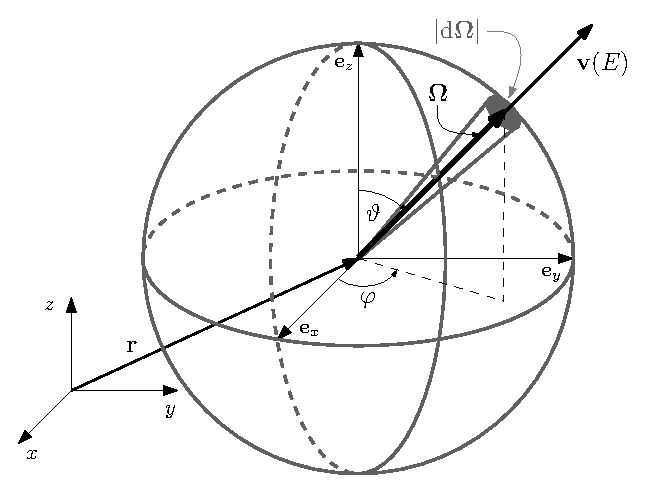
\includegraphics[scale=1]{phase_space.eps}
    \caption[Phase space of neutrons]{Phase space of neutrons}
    \label{fig:phase_space}
\end{figure}%
The product measure
\begin{equation}\label{eq:measure}
  \d{x} = \d{\mu(X)} = \d{\mu(V\times\Sphere\times [\Emin,\Emax])} = \d{\br}\d{\bomega}\d{E}
\end{equation}
is used when integrating over $X$, 
while the boundary measure
\begin{equation}\label{eq:measure2}
\db = \abs{\bomega\cdot\bn}\d{\gamma}\d{\bomega}\d{E},\quad \d{\gamma} = \d{\mu(\pV)},
\end{equation}
is used when integrating over $\pX[\pm]$. When refering to physical units, we will consider the length scale of $\VV$ in
centimeters.

\comment{
When discussing various semi-discretizations of the NTE, we will also refer to the following subspaces  (``sections''
through the phase space):
\begin{equation}\label{eq:pssec}
	X_E := \{(\br,\bomega,E):\ \br\in \VV\subset\R[3], \bomega\in \Sphere, E \in [\Emin,\Emax]\}
\end{equation}
}

Since the direction vectors are confined to the sphere, we can express the three
Cartesian components of $\bomega$ by only two spherical coordinates $\polar\in[0,\pi]$ and
$\azimuthal\in[0,2\pi)$\nomenclature[g]{$\polar$}{polar angle}\nomenclature[g]{$\azimuthal$}{azimuthal
angle}:
\begin{equation*}
	\bomega = \left[\begin{array}{c}
		\Omega_x \\
		\Omega_y \\
		\Omega_z
	\end{array}\right] = \left[\begin{array}{c}
		\sint\cosp \\
		\sint\sinp \\
		\cost
	\end{array}\right]
\end{equation*}
(see \fref{fig:streaming}).
\begin{figure}[!hbt]
    \centering
    \includegraphics[scale=1.275]{cartesian_streaming}
    \caption[Cartesian coordinate system]{Cartesian coordinate system}
    \label{fig:streaming}
\end{figure}
To transform integrals with respect to $\d{\bomega}$ into double integrals with respect to $\polar$ and $\azimuthal$,
note that the solid angle $\d{\bomega}$ subtended at the center of $\Sphere$ by the spherical differential element
$\abs{\d{\bomega}}$ can be written as:
$$
	\d{\bomega} = \frac{\abs{\d{\bomega}}}{r^2} = \frac{r^2 \sint \d{\polar}\d{\azimuthal}}{r^2} =  \sint
	\d{\polar}\d{\azimuthal} $$
(see \fref{fig:element}).
\begin{figure}[!hbt]
    \centering
    \includegraphics[scale=1.275]{element}
    \caption[Solid angle]{Schematic of the (scaled) solid angle of directions}
    \label{fig:element}
\end{figure}
We will also need to integrate functions that depend on the cosine of the angle between two 
directions $\bomega$ and $\bomega'$. We shall denote this angle and its cosine by $\polar_0$ and $\mu_0$, respectively
(see \fref{fig:scatter} in appendix for geometrical interpretation).
Then
$$
	\mu_0 \equiv \cos \polar_0 = \bomega\cdot\bomega'
$$
and
\begin{equation}\label{eq:invint}
\begin{aligned}
	\intA[']{f(\bomega\cdot\bomega')} &= \int_{0}^{2\pi} \int_{0}^{\pi}
		f(\cos \polar_0) \sin \polar_0\d{\polar_0} = 2\pi \muint[_0]{f(\mu_0)}\\
		&= \intA{f(\bomega'\cdot\bomega)}
\end{aligned}
\end{equation}
Notice that the result depends on neither $\bomega$ nor $\bomega'$.

\section{Steady state neutron transport in isotropic bounded domain}\label{sec:NTE}
In most practical cases, we can assume that the medium in which we study neutron transport is isotropic.
The first consequence of this assumption is that 
$$
	\sigma_t(\br,\bomega,E)\psi(\br,\bomega,E) \equiv \sigma_t(\br,E)\psi(\br,\bomega,E)
$$ 
for any $\bomega\in\Sphere$. The
second is that reactions that change the direction of neutrons from $\bomega'$ to $\bomega$ are
invariant under rotation of the coordinate system and are thus completely determined by the cosine of the two vectors:
\begin{equation}\label{eq:iso}
	\kappa(\cdot,\bomega\sla\bomega',\cdot) \equiv \kappa(\cdot,\bomega\cdot\bomega',\cdot).
\end{equation}
The steady state NTE \eqref{eq0} in this regime reads
\begin{equation}\label{eq1}
\begin{multlined}
  \bomega\cdot\nabla\psi(\br,\bomega,E) + \sigma_t(\br,E)\psi(\br,\bomega,E) =\\[.25em]
   = \intE[']{\Emin}{\Emax}{
      \intA[']{\kappa(\br,\bomega\cdot\bomega',E\sla E')\psi(\br,\bomega',E')}
    } + q(\br,\bomega,E)
 \end{multlined}
\end{equation}
in $X$, complemented by specified angular flux distribution at $\pX[-]$. The two prototypical inflow boundary
conditions are:
\begin{itemize}
	\item incoming angular neutron flux
	\begin{equation}\label{eq:nte2}
	  \psi\vert_{\pX[-]} = \psi_{\text{in}}
	\end{equation}
	($\psi_{\text{in}}\equiv 0$ corresponds to vacuum in $\R[3]\setminus \overline V$, which is a common
	 assumption in nuclear reactor modeling),
	
	\item albedo boundary reflection
	\begin{equation}\label{eq:nte3}
  	\psi(\br,\bomega,E) = \alpha(\br)\psi(\br, \bomega_R, E),\quad (\br,\bomega,E)\in \pX[-],\ \ \bomega_R = \bomega - 2
  	\bn (\bomega \cdot \bn)
  \end{equation}
  where $\bomega$ is the reflection of $\bomega_R$ about the boundary plane. For $\alpha \equiv 1$, this corresponds to
  complete specular reflection and is used to model planes of symmetry, while for $\alpha =
  0$, we recover the vacuum condition from above. Intermediate values mean that a fraction of neutrons leaving the
  domain in direction $\bomega_R$ are returned back in direction $\bomega$, which is commonly used to model reactor
  reflectors. We thus assume $0 \leq \alpha \leq 1$. 
\end{itemize}
\begin{remark}
	The albedo coefficient $\alpha$ may in general vary with the reflector properties and should also capture 
	redistribution of the reflected neutrons within the phase space due to their diffusion through the reflector. A general
	treatment of albedo condition is given in \cite{Sanchez4} (see also \cite{Sanchez3}), where an integral albedo operator
	$\beta$ is introduced, such that
\begin{equation}\label{eq:albedo-general}
	\angflux(x)\big\vert_{\pX[-]} = (\beta\angflux)(x) = \bndint[']{\pX[+]}\beta(x\sla x')\angflux(x'),
\end{equation}
	where $x = (\br,\bomega,E)$ and $x' = (\br',\bomega',E')$. 
\end{remark}
For formal description of other types of boundary conditions, we refer to \cite{Sanchez4} or \cite[Sec. 1.3]{Agoshkov}.

A physically plausible solution of NTE should be moreover non-negative throughout $\VV$ and continuous along any
direction $\bomega$, i.e. $\psi(\br + s\bomega,\bomega,E)$ is a continuous function of $s$ for any $\br$, $\bomega$, $E$. Note
that $\psi(\br + s\bomega',\bomega,E)$ \textsl{may} be discontinuous when $\bomega' \neq \bomega$.

\subsection{Advection term}\label{sec:advection}
In Cartesian coordinate system (that we will exclusively consider in this thesis),
$$
	\bomega\cdot\nabla\angflux = \bomega_x\pd{\angflux}{x} + \bomega_y\pd{\angflux}{y} + \bomega_z\pd{\angflux}{z} = 
	\der{x}{s}\pd{\angflux}{x} + \der{y}{s}\pd{\angflux}{y} + \der{z}{s}\pd{\angflux}{z} = \der{\angflux}{s},
$$
where $s\in I\subset \R$ parametrizes the path traveled by the neutron along the direction $\bomega$ (the
\textit{characteristic}, see \fref{fig:cartesian2}).
\begin{figure}[htp]
\begin{center}
  \includegraphics[scale=1.2]{cartesian_streaming2}
  \caption{Characteristic direction in the Cartesian coordinate system}
  \label{fig:cartesian2}
\end{center}
\end{figure}
Assuming now for simplicity that the integral term on the right of \eqref{eq1} is absorbed in the source term $q$, we
may invert the differential operator on the left of \eqref{eq1} by integration along these characteristics and obtain an
integral formulation of the neutron transport equation:
\begin{equation}\label{eq:nte-integral}
	\angflux(\br,\bomega) = \angflux(\br_0,\bomega)e^{-\tau(\br,\br_0)} + \int_0^{s_0}
	q(\br',\bomega)e^{-\tau(\br,\br')}\,\d{s'}
\end{equation}
where
\begin{align}
	\br' &= \br - s' \bomega, \quad \br_0 = \br - s_0 \bomega\nonumber\\[.2em]
	\tau(\br,\br') &= \tau(\br,\br-s'\bomega) = \int_0^{s'} \sigma_t(\br - s''\bomega)\,\d{s''} \label{eq:tau}
\end{align}
In reference to \fref{fig:trepka}
\begin{figure}[hbp]
\begin{center}
  \includegraphics[scale=.75]{trepka}
  \caption{Illustration for the solution on a characteristic}
  \label{fig:trepka}
\end{center}
\end{figure}
we can interpret the first term on the right of \eqref{eq:nte-integral} as the number of
neutrons moving in the direction $\bomega$ that entered the given volume in $\br_0$ and reached point $\br$ without
collision, whereas the second term as the number of neutrons introduced into the characteristic direction by sources 
between $\br_0$ and $\br$ and reaching $\br$ without collision. The \textit{optical path length} $\tau$ represents the 
probability of collision between $r'$ and $r$. This integral form is of both theoretical and practical value, as we will
see later in sections \ref{sec:fixed-source} and \ref{sec:lattice}.

\subsection{Collision terms}
The kernel of the integral operator on the right-hand side of \eqref{eq1} can be split into the so-called
\textit{double-differential macroscopic cross-section} for scattering and fission, respectively:
\begin{equation}\label{eq:splitting}
  \kappa(\br,\bomega\cdot\bomega',E\sla E') = \sigma_s(\br,\bomega\cdot\bomega',E\sla E') +
  \sigma_f(\br,\bomega\cdot\bomega',E\sla E').
\end{equation}
These cross-sections characterize the mean number of ($\bomega$, $E$)-neutrons coming out of a (possible) collision of 
($\bomega'$, $E'$)-neutrons with nuclei at $\br$ (or more precisely in a
differential element around $\br$). Such collisions can either just change the direction and energy of the
inducing neutrons (elastic scattering) or cause absorption of the neutrons followed by release of
new ones in the considered direction and energy range (fission), or both (inelastic scattering).
Ordinary macroscopic cross-sections $\sigma_s(\br,E)$, $\sigma_f(\br,E)$ are then introduced to characterize the total
probability that neutrons undergo collisions of the above type irrespective of the outgoing direction, i.e.
\begin{equation}\label{eq:ddifxs}
\begin{aligned}
\eta\sigma_s(\br, E) &= \intE[']{\Emin}{\Emax}{\intA{\sigma_s(\br,\bomega\cdot\bomega', 
	E'\sla E)}},\\
\nu\sigma_f(\br, E) &= \intE[']{\Emin}{\Emax}{\intA{\sigma_f(\br,\bomega\cdot\bomega', 
	E'\sla E)}}
\end{aligned}
\end{equation}
where $\eta$ and $\nu$, respectively, are the mean (net) number of neutrons coming out of the scattering event ($=1$ in
case of elastic scattering, might be $> 1$ when elastic scattering takes place) and the fission event, respectively. 

The \textit{total macroscopic cross-section}, $\sigma_t$, characterizing the probability that neutron with energy $E$
undergoes a collision of any type with nuclei at $\br$, can now be decomposed as 
\begin{equation}\label{eq:st}
  \sigma_t(\br,E) = \sigma_c(\br,E) + \sigma_f(\br,E) + \sigma_s(\br,E) \equiv \sigma_a(\br,E) + \sigma_s(\br,E)
\end{equation}
where
\begin{itemize}
	\item $\sigma_c(\br, E)$ is the non-productive capture cross section (resulting in no new neutrons being introduced
	into the system) and
  	\item $\sigma_a(\br, E) = \sigma_c(\br,E) + \sigma_f(\br,E)$ is the absorption cross section.
\end{itemize}

For later use, note that fission is an isotropic process (which removes the angular dependence of the
double-differential fission cross-section altogether) and the new energy distribution does not depend on the energy of 
the inducing neutron 
\begin{figure}[hbt]
\begin{center}
  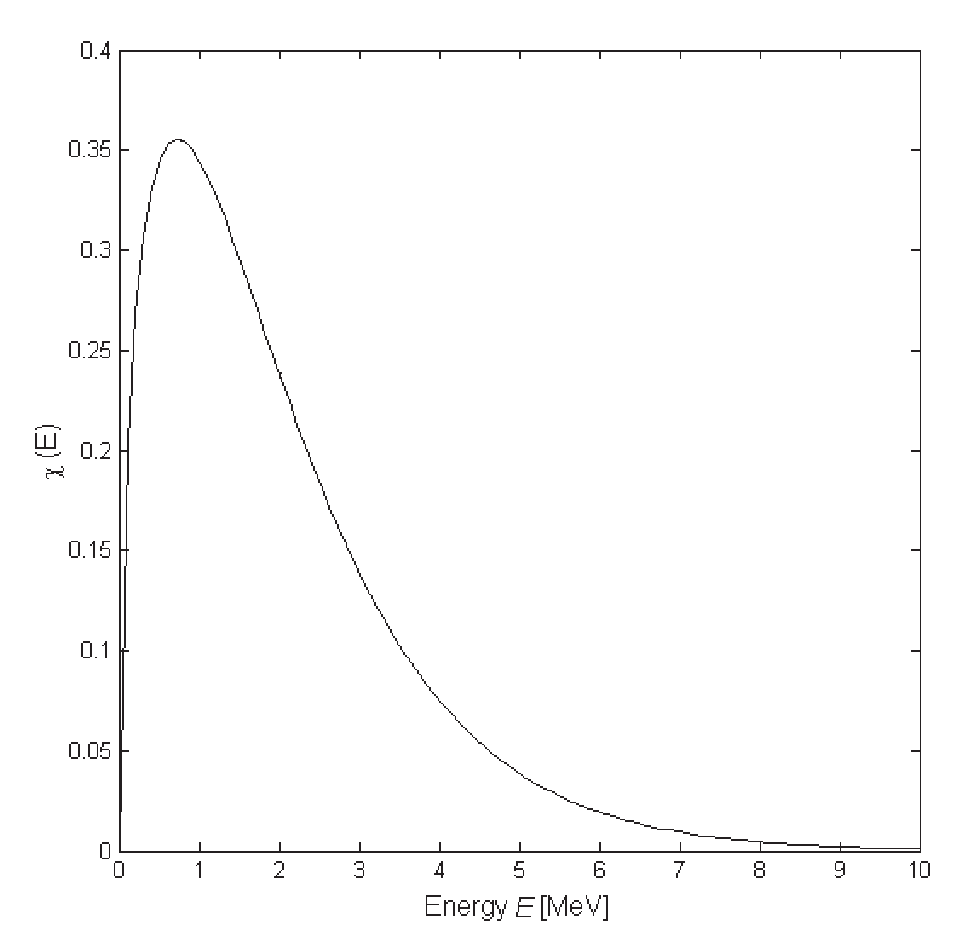
\includegraphics[scale=.6]{spectrum}
  \caption{Energy spectrum of (prompt) neutrons released from fission of U235}
  \label{fig:spectrum}
\end{center}
\end{figure}
(as it corresponds to the neutrons originally bound inside the nucleus; \fref{fig:spectrum}
shows a typical shape of that function); using the second eq.
\eqref{eq:ddifxs}, we can then write:
\begin{equation}\label{eq:sf}
\sigma_f(\br,\bomega\cdot\bomega',E\sla E') = \frac{\chi(E)\nu\sigma_f(\br,E')}{4\pi},\quad 
\intE[']{\Emin}{\Emax}{\chi(E')} = 1.
\end{equation}
 
A physically realistic assumption is that all the macroscopic cross-sections are bounded measurable functions
 \footnote{with respect to product measure of type \eqref{eq:measure} appropriate for their particular set of arguments,
 or with respect to $\d{\mu(V\times\Sphere^2\times [\Emin,\Emax]^2)}$ in case of double-differential cross-section},
 piecewise continuous in $\VV$. The unit of macroscopic cross-sections is \SI{}{cm^{-1}}.

\subsection{Quantities of interest}\label{sec:qoi}
From the solution of eq. \eqref{eq1}, one can derive the following important integral quantities
\begin{itemize}
  \item \textit{scalar neutron flux density} \SI{}{[cm^{-2}.s^{-1}]}
  \begin{equation}\label{eq:scalar_flux}
    \phi(\br, E) = \intA{\psi(\br,\bomega,E)},
  \end{equation}
  \item \textit{net neutron current density} \SI{}{[cm^{-2}.s^{-1}]}
	\begin{equation}\label{eq:bJ}
		\bJ(\br, E)	= \intA{\bomega\psi(\br,\bomega,E)},
	\end{equation}
\end{itemize}
so that integrating $\bJ(\br,E)\cdot\bn(\br)$ over a given surface 
gives the total number of neutrons with energy $E$ crossing (per unit time) that surface in the direction of 
$\bn$ (and allows us to assess neutron conservation within given volume, recall Remark \ref{rem:balance}).

The integral
\begin{equation}\label{eq:rr}
  \intE{E_1}{E_2}{\sigma_x(\br, E) \phi(\br, E)}
\end{equation}
represents the \textit{reaction rate density} (per unit time) of given type ($x = t,a,f,s,c$, see \eqref{eq:st}), 
induced by neutrons of energies in range $[E_1, E_2]$. 
As well as the scalar flux itself, reaction rates may be experimentally measured
by various detector mechanisms, which is the reason why these quantities are more important in practical calculations
than the actual solution of the NTE (the angular neutron flux). Of particular importance for reactor calculations is the
\textit{power density} 
\begin{equation}\label{eq:power}
	P(\br) = \intE{\Emin}{\Emax}{e\sigma_f(\br, E) \phi(\br, E)} \quad \SI{}{[W.cm^{-3}]}
\end{equation}
where $e$ is the energy conversion factor converting fission rate to watts.

\subsection{Solvability of neutron transport problems}\label{sec:ntp}
In this section, we will formulate the two basic problems of neutron transport in an operator form.
We will consider the generalized statements in which the equation and boundary conditions are assumed to be satisfied a.e. in $X$ and
$\bomega\cdot\nabla$ represents the generalized derivative in the usual Sobolev sense. This is motivated by the low
regularity that can be expected from the exact solution of the NTE -- for example, even for piecewise smooth material data
(cross-sections $\sigma_x$) and sources $q$, the solution of the NTE is known to possibly exhibit singularities in 
first partial derivatives (or be discontinuous as a function of $\bomega$) at surfaces of material discontinuities 
coinciding with characteristic curves of the left-hand side of \eqref{eq1} (that is, straight lines; see \cite[Chap.
1]{Agoshkov}, \cite[Sec. III]{Vladimirov}).



\subsection{Neutron transport problem with fixed sources}\label{sec:fixed-source}
Let us introduce the standard spaces of Lebesgue-integrable functions (w.r.t. the product measure \eqref{eq:measure},
resp. \eqref{eq:measure2}) 
\begin{equation}\label{eq:Lp}
\nomenclature[a]{$\Lp(X)$}{space of functions integrable in the Lebesgue sense with their $p$-th power over
$X$\nomrefeq}
\nomenclature[a]{$\Lp_\sigma(X)$}{space weighted with the total cross-section $\sigma_t$\nomrefeq}
\begin{aligned}
	\Lp(X) &= \left\{\psi\mid \norm[\Lp(X)]{\psi} := \left(\int_X\abs{\psi(x)}^p\,\d{x}\right)^{1/p} <
	\infty\right\},\quad 1\leq p < \infty,\\
	\Lp(\pX[\pm]) &= \left\{\psi\mid \Vert\psi\Vert_{\Lp(\pX[\pm])} :=
	\left(\int_{\pX[\pm]}\abs{\psi(x)}^p\,\db\right)^{1/p} < \infty\right\},\quad 1\leq p < \infty,\\
	\Lp[\infty](X) &= \{\psi\mid \norm[L^{\infty}(X)]{\psi} := \esssup_{X} \abs{\psi(x)} < \infty\}\\
	\Lp[\infty](\pX[\pm]) &= \{\psi\mid \Vert\psi\Vert_{L^{\infty}(\pX[\pm])} := \esssup_{\pX[\pm]}
	\abs{(\bomega\cdot\bn)\psi(x)}< \infty\}
\end{aligned}
\end{equation}
Note that for the total volumetric scalar flux to be finite  (as is physically expected), the solution should belong to
$\Lp[1](X)$.

We formulate the fixed source problem using the following operators:
\begin{equation*}
  \begin{gathered}
    A\psi(\br,\bomega,E) = \bomega\cdot\nabla\psi(\br,\bomega,E),\\%[.85em]
    \Sigma_t\psi(\br,\bomega,E) = \sigma_t(\br,E)\psi(\br,\bomega,E),\\%[.75em]
    K\psi(\br,\bomega,E) = \intE[']{\Emin}{\Emax}{
            \intA[']{\kappa(\br,\bomega\cdot\bomega',E\sla E')\psi(\br,\bomega',E')}
          }.
  \end{gathered}
\end{equation*}
We shall call $A$, $\Sigma_t$, $K$ and $T = A + \Sigma_t - K$ the \textit{advection}, \textit{reaction}, 
\textit{collision} and \textit{transport} operator, respectively. All these operators are continuous; the reaction
operator $\Sigma_t : \Lp(X) \to \Lp(X)$ is a simple multiplication operator in $\Lp(X)$, self-adjoint and bounded,
while the operator $K: \Lp(X) \to \Lp(X)$ is bounded under additional (physically justifiable) conditions
(e.g. conditions (c) and/or (d) of the following theorem, depending on the chosen $p$; cf. also Lemma
\ref{lem:Kbounded} below), but is self-adjoint if and only if the kernel $\kappa$ of $K$ is symmetric in $E$ and $E'$. 
With the exception of the mono-energetic case, this is generally not true (a fact to which we return again in \sref{sec:MG}). 

For piecewise smooth
$\pV$ and $1\leq p < \infty$, the traces $\gamma\psi \equiv \psi\vert_{\pX[\pm]}\in\Lp(\pX[\pm])$ are well defined for
functions $\psi\in \widehat H^p(X)$, where
$$
\widehat H^p(X) = \{\psi\mid \psi\in\Lp(X), \bomega\cdot\nabla\psi\in\Lp(X)\}, \quad 1 \leq p \leq \infty
$$
and a continuous lifting operator $\mathcal{G}: \psi_{\text{in}}\in\Lp(\pX) \mapsto \widetilde\psi \in \widehat H^p(X)$
exists (\cite[Thm. 1, Appendix of \S 2, Chap. XXI]{DautrayLions}, \cite{Boulanouar1} for the case $p = \infty$). Let us 
then define the Sobolev space of functions with bounded boundary traces
\begin{equation}\label{eq:Hp}
  \nomenclature[a]{$\Hp{p}(X)$}{Sobolev space of functions whose (generalized) partial derivatives up to order $k$ are
 in $\Lp{p}$.\nomrefeq} 
 \Hp(X) := \left\{\psi\in\Lp(X), \bomega\cdot\nabla\psi\in\Lp(X), \Vert\gamma\psi\Vert_{\Lp(\pX)} < \infty\right\}. 
\end{equation}
Note that the lifting operator allows us to convert a problem $T\psi = q$ with non-homogeneous boundary conditions 
\eqref{eq:nte2}\footnote{Results for the reflective or more general boundary conditions require special trace theorems, see 
\cite[Chap. XXI, Appendix of \S2]{DautrayLions} or \cite[Chap. 2]{Agoshkov}.} to a problem 
$$
	T(\psi - \widetilde\psi) = q - T\widetilde\psi
$$ 
where trace of the new unknown function $u = \psi - \widetilde\psi$ on $\pX[-]$ vanishes. Therefore, we can focus on the
case with homogeneous conditions. 



We will first consider the physically most natural $\Lp[1](X)$ setting.
\begin{theorem}\label{thm1}
Assume that
\begin{enumerate}[label=(\alph*)]
	\item $\sigma_t \in \Lp[\infty](X)$, $\sigma_t \geq \mst > 0$ a.e. in $\VV\times[\Emin,\Emax]$,
	\item $\kappa \geq 0$ a.e. in $\VV\times\Sphere^2\times[\Emin,\Emax]^2$,
	\item $\displaystyle c(x) < 1$ a.e. in $X$, where
	  \begin{equation}\label{eq:c}
	    c(\br,E) := \frac{1}{\sigma_t(\br,E)}\int_{\Emin}^{\Emax}\int_{\Sphere} \kappa(\br,\bomega\cdot\bomega',
	    E'\sla E)\,\d{E'}\d{\bomega'}.
	  \end{equation}
\end{enumerate}
Then the fixed source, steady state neutron transport problem with vacuum boundary conditions 
\begin{equation*}
  \left\{
  \begin{aligned}
     &T\psi(\br,\bomega,E) = q(\br,\bomega,E),\\
     &\Dom{T} = \{\psi\in \Hp[1](X),\ \psi\vert_{\pX[-]} = 0\},
  \end{aligned}
  \right.
\end{equation*}
has a unique solution $\psi(\br,\bomega,E)\in\Dom{T}\subset\Lp[1](X)$ for any $q\in \Lp[1](X)$.
\end{theorem}
\begin{proof}
\cite[Chap. XXI, \S 2, Proposition 5]{DautrayLions}
\end{proof}

The value $c$ in Thm. \ref{thm1} has the physical meaning of the average number of neutrons emitted (in all possible
directions and energies) after a neutron with energy $E$ (coming from any direction) collides with a nucleus at point
$\br\in V$.\footnote{\label{ftn:c}Notice that (using \eqref{eq:ddifxs})
$
	c\sigma_t(\br,E)\equiv c(\br,E)\sigma_t(\br,E) = \eta\sigma_s(\br,E) + \nu\sigma_f(\br,E).
$}
Condition (c) thus expresses the requirement that the system be \textit{subcritical} in order for a
steady solution in presence of external sources to be achieved (the notion of criticality will be formally introduced in the following
subsection).

Dautray and Lions in 
\cite[\S2, Chap. XXI]{DautrayLions} also outline the proof based on the same ideas (the theory of monotone 
operators)\footnote{For a different approach, we refer to \cite[Chap. 3]{Agoshkov}, where the $\Lp[2](X)$ case has been extensively studied via variational methods.} in
general $\Lp(X)$ spaces for $1 < p < \infty$, where in particular the case $p = 2$ is important\footnote{even though it does not lead to a direct 
physical interpretation as the $\Lp[1](X)$ setting} as the Hilbert space structure of $\Lp[2](X)$ allows to use richer 
set of mathematical tools to formulate practical solution methods (like those based on Fourier transform or the finite 
element methods). In this case, however, we need to add to assumptions (a-c) another assumption
\begin{enumerate}
  \item[(d)] $d(x) < 1$ a.e. in $X$, 
\end{enumerate}
where
\begin{equation}\label{eq:d} 
d(\br,E) := 
  \frac{1}{\sigma_t(\br,E)}\int_{\Emin}^{\Emax}\int_{\Sphere} \kappa(\br,\bomega\cdot\bomega',
	    E\sla E')\,\d{E'}\d{\bomega'}
\end{equation}
can be interpreted as the average number of neutrons emitted with energy $E$ (into any direction) from
collisions induced by all possible neutrons impinging on the nucleus at $\br$ (again, this is a reasonable condition
in the subcritical state). Note that because angular dependence of $\kappa$ is only through the cosine of the collision
angle ($\bomega\cdot\bomega'$), assumptions (c) and (d) really represent different assumptions about just the energy
transfer in collisions.

In Proposition 6, Dautray and Lions also 
state the existence of unique solution in $\Lp[\infty](X)$ for $q\in \Lp[\infty](X)$; the proof in this case is based on
 the inversion of the transport operator along characteristics (see \ref{sec:advection} above) and uses condition (d)
 instead of (c).
 The approach based on the characteristic form of the NTE has also been used by Sanchez in \cite{Sanchez3}, who proved  
 existence and uniqueness of solution in the cross-section weighted space $\Lp[1]_{\sigma}(X)$.
 This appears to be an alternative physically natural functional setting due to the definition of the reaction rate, eq. 
 \eqref{eq:rr}; moreover, assumption (a) may be relaxed by allowing $\sigma_t = 0$ in arbitrarily large regions 
  (the \textit{void regions}). Note that if we assume (a) of Thm. \ref{thm1}, the norms of $\Lp[1]$ and
  $\Lp[1]_{\sigma}$ are equivalent and the measure $\d{\tau} = \sigma_t(x) \d{x}$ associated with the space
  $\Lp[1]_{\sigma}$ represents a differential optical path length (see eq. \eqref{eq:tau}).
  
\subsubsection{$\Lp[2](X)$ setting}

Let us now make a short stop in the $\Hp[2](X)$ space and quote some results that we will make use of later. This is a
Hilbert space when equipped with the inner product
$$
	\ip[\Hp[2](X)]{f,g} := \ip[\Lp[2](X)]{\bomega\cdot\nabla f, \bomega\cdot\nabla g} + \ip[\Lp[2](X)]{f,g} +
	\ip[\Lp[2](\pX)]{f,g} 
$$
where
\begin{equation}\label{eq:ipL2}
	\ip[\Lp[2](X)]{f,g} = \int_X f g \d{x},\quad  \ip[\Lp[2](\pX)]{f,g} f g \d{\xi}
\end{equation}
Let us denote 
\begin{equation}\label{eq:opL}
	$\op{L} := A + \Sigma_t$.
\end{equation}
Using the Poincar{\' e}-Friedrichs inequality and integration by parts (see e.g. \cite[Chap.
2]{Agoshkov}), one can show the following:
\begin{lemma}\label{lem:Lcoercive}
	Assume (as in item (a) in Thm. \ref{thm1}) that 
	$$
		0 < \mst \leq \sigma_t \leq \Mst \ \text{a.e. in } \VV\times[\Emin,\Emax].
	$$
	Then the operator $\op{L} : \Hp[2](X) \to \Lp[2](X)$ is
	bounded and coercive with constants $\Mst$ and $\mst$, respectively: 
	$$
		\ip[\Lp[2](X)]{Lu, u} \geq \mst \norm[\Lp[2](X)]{u}^2,\quad  \norm[\Lp[2](X)]{Lu} \leq \Mst \norm[\Lp[2](X)]{u}^2.
	$$
\end{lemma}
Also, as a consequence of H\"older inequality, the collision operator $\op{K} : \Lp[2](X) \to \Lp[2](X)$ is
bounded:
\begin{lemma}[\cite[Lemma 1, \S 3, Chap. XXI]{DautrayLions}]\label{lem:Kbounded}
	Assume that there exist $M_a > 0$, $M_b > 0$, such that for a.e. $(\br,E) \in \VV\times[\Emin,\Emax]$
	$$
	\int_{\Emin}^{\Emax}\int_{\Sphere} \kappa(\br,\bomega\cdot\bomega',
	    E'\sla E)\,\d{E'}\d{\bomega'} \leq M_a,\quad
	\int_{\Emin}^{\Emax}\int_{\Sphere} \kappa(\br,\bomega\cdot\bomega',
	    E\sla E')\,\d{E'}\d{\bomega'} \leq M_b.    
	$$
	Then 
	$$
	\norm[\Lp[2](X)]{Ku} \leq M_a^{\frac12} M_b^{\frac12} \norm[\Lp[2](X)]{u}.
	$$
\end{lemma}
\begin{remark}
	Note that from \eqref{eq:c} and \eqref{eq:d}, 
	$$
	M_a = \esssup_{\VV\times[\Emin,\Emax]} c(\br,E)\sigma_t(\br,E), \quad M_b = \esssup_{\VV\times[\Emin,\Emax]}
	d(\br,E)\sigma_t(\br,E). 
	$$
\end{remark}
These results may be used to establish coercivity and boundednes of the transport operator 
$T = L - K$ and prove well-posedness in the $\Lp[2](X)$ setting via the Lax-Milgram lemma. Although this follows rather
straightforwardly from the assumptions (a-d) above, we won't go into details; nevertheless, we state the Lax-Milgram
lemma here for the purposes of \sref{sec:SI}. We state it in its general form for an operator $\genop{A}$ being an 
element of space $\mathcal{L}_{V,V'}$ of bounded linear operators acting from $V$ to its dual $V'$.
\begin{lemma}[Lax-Milgram]
	Let $\genop{A}\in\mathcal{L}_{V,V'}$ be a bounded and coercive operator with constants $C_b$ and $C_c$, respectively.
	Then for any $f\in V'$, there exists a unique $u\in V$ such that
	$$
		\langle Au, v \rangle = \langle f, v \rangle  \quad \forall v\in V,
	$$
	and
	$$
		\norm[V]{u} \leq \frac{1}{C_c}\norm[V']{f}.
	$$
\end{lemma}
In our case, $V = \Hp[2](X)$, $\genop{A} \equiv T : V \to \Lp[2](X) \subset V'$ and the duality pairing
$\langle \cdot,\cdot\rangle$ coincides with the $\Lp[2](X)$ inner product. %We only note that considering $T:V\toV'$ (thus
%allowing more general right-hand sides) is possible, but we don't go into details here.


\subsection{Criticality problem}\label{sec:criticality}

The other important problem in neutron transport (particularly in nuclear reactor engineering) requires the
determination of material composition (i.e. the values of $\sigma_x$) for a given domain geometry (or vice versa)
which ensures a steady neutron distribution (that means -- steady power generation) with no additional neutron sources
than the fission. This is called a ``criticality problem'' -- the system is said to be \textit{subcritical},
\textit{supercritical} and \textit{critical}, respectively, if without an additional neutron source the number of
neutrons in the core will, respectively, continuously diminish, increase or be maintained through the
balance between actual out of core leakage, absorption and fission. In reactor core reloading optimization, we assume
the core geometry fixed and try to find such a material composition that (besides other optimization criteria) would
ensure the critical state. 

Mathematically, we are looking for a non-trivial non-negative solution of the homogeneous
version of eq. \eqref{eq1} (i.e. with $q\equiv 0$ and b.c. \eqref{eq:nte3}), which means solving an eigenvalue
problem. The resulting eigenvalue then describes the departure from critical state with the current set of material
data and the associated eigenfunction represents the shape of neutron flux in such a steady state. 

In order to formulate
the eigenvalue problem, we split the kernel of the collision operator according to \eqref{eq:splitting} into the 
scattering and fission part, thus
$$
K\psi(\br,\bomega,E)
  			= S\psi(\br,\bomega,E) + F\psi(\br,\bomega,E)
$$
where, using further eq. \eqref{eq:sf},
\begin{equation}\label{eq:FScrit}
\begin{aligned}
F\psi(\br,\bomega,E) &= \frac{\chi(E)}{4\pi}\intE[']{\Emin}{\Emax}{\nu\sigma_f(\br,E')\intA{\psi(\br,\bomega,E')}}\\
S\psi(\br,\bomega,E) &= \intE[']{\Emin}{\Emax}{\intA[']{\sigma_s(\br,\bomega\cdot\bomega',E\sla
E')\psi(\br,\bomega,E')}}
\end{aligned}
\end{equation}
The criticality eigenvalue problem then reads:\\
\textit{Find nontrivial, nonnegative $\psi(\br,\bomega,E)\in \Dom{B}$ and $\lambda > 0$, such that}
\begin{equation}\label{eq:critical}
\left\{
  \begin{aligned}
     &B\psi(\br,\bomega,E) \equiv \bigl[A + \Sigma_t - S]\psi(\br,\bomega,E) = \frac{1}{\lambda} F\psi(\br,\bomega,E),\\
     &\Dom{B} = \{\psi\in \Hp(X),\ \psi\vert_{\pX[-]} = \beta\psi\},
  \end{aligned}
\right.
\end{equation}
\textit{where $\beta\psi$ is given by the right-hand side of \eqref{eq:nte3} (or, more generally, $\beta$ is the
boundary operator of \eqref{eq:albedo-general})}.  

Proving existence and uniqueness of solution of \eqref{eq:critical} can proceed in the following sequence:
\begin{enumerate}
	\item
		Prove that the transport operator $B$ is invertible. This permits the traditional transcription of the  eigenvalue
		equation \eqref{eq:critical}:
		$$
		B^{-1}F\angflux = \lambda\angflux.
		$$
		Results of the previous section can be used here if we consider the collision kernel $\kappa$ without the fission
		part, e.g. if instead of the average number of all emitted neutrons in \eqref{eq:c} we consider only the number
		emitted from scattering collisions: 
		\begin{equation}\label{eq:tildec}
		\tilde c(\br,E) := \frac{1}{\sigma_t(\br,E)}\int_{\Emin}^{\Emax}\int_{\Sphere}
		\sigma_s(\br,\bomega\cdot\bomega', E'\sla E)\,\d{E'}\d{\bomega'}.
	    \end{equation}
	\item
		Prove that operator $B^{-1}F$ is (strongly) positive and compact. As such, it has countably many eigenfunctions. 
		Positivity can be deduced from physical properties of the involved operators (although this may place much too severe
		restrictions on the coefficients, see below). Compactness is harder to establish and holds in general in $\Lp(X)$
		spaces for $1 < p < \infty$, but not for $p = 1$ or $p = \infty$ (we will comment on this case below).
	\item
		Invoke the Krein-Rutmann theorem for positive linear compact operators (e.g., \cite[Thm. 5.4.33]{DrabekNFA}) to prove
		that the spectral radius of $B^{-1}F$ is a simple eigenvalue associated with the unique positive eigenfunction.
\end{enumerate}
\begin{remark}\label{rem:keff}
In nuclear engineering, spectral radius of $B^{-1}F$ is often denoted $\keff$
and called \textit{effective multiplication factor}. Physically,
$$
\keff \equiv \frac{\mbox{neutron emission}}{\mbox{neutron loss}}
$$
so that 
$\keff < 1$, $\keff > 1$ and $\keff = 1$, respectively, correspond to \textit{subcritical},
\textit{supercritical} and \textit{critical} system. Notice that $\keff < 1 \Rightarrow c < 1$, but not the other way
round because the possibility of neutron loss due to out of core leakage is not included in \eqref{eq:c}. 
\end{remark}
\begin{remark}
As in footnote \ref{ftn:c}, using definition \eqref{eq:ddifxs} and further absorbing $\eta$ into
$\sigma_s$, we can rewrite \eqref{eq:tildec} as a ratio 
\begin{equation}\label{eq:scattering_ratio}
\tilde{c}(\br,E) = \frac{\sigma_s(\br,E)}{\sigma_t(\br,E)},
\end{equation}
which is commonly called \textit{scattering ratio} in nuclear engineering and transport theory texts (e.g.,
\cite{Adams}).
\end{remark}

Because of the first step, we can expect similiar assumptions as in Thm. \ref{thm1} (or in the discussion below the
theorem) to be required. Depending on the chosen functional setting, various additional assumptions need to be made in
order to carry out the other two steps.
These mathematical assumptions restrict either the boundary conditions, geometry or material composition of the solution
domain, or energetic dependence (or all) and may not always coincide with physical reality. For instance, strong
positivity of $B^{-1}F$ would require $\sigma_f \geq \underline{\sigma_f} > 0$ a.e. in $X$%
\nomenclature[g]{$\underline{\sigma_t}$}{minimum value attained by $\Sigma_f$}% 
, implying
that fission occurs everywhere, which it generally does not (consider for instance the area between fuel rods in nuclear
reactors, filled with coolant water). For only a non-strongly positive compact operator, one can still use the weak form
of the Krein-Rutmann theorem (\cite[Prop. 5.4.32]{DrabekNFA}). That theorem however does not guarantee uniqueness of the
eigensolution and a separate demonstration is required. In $\Lp[1](X)$ or $\Lp[\infty](X)$, compactness of $B^{-1}F$ can
be replaced by power compactness, i.e. $(B^{-1}F)^2$ (\cite{Sanchez3}).

In \cite{Sanchez3}, the above scheme is carried out in the weighted $\Lp[1]_{\sigma}$ setting introduced in previous
section. The result is the following theorem:

\begin{theorem}\label{thm:eigenvalue}
	Let $\tilde{c} < 1$ a.e. in $X$ and either $\sigma_f \geq \tilde{\sigma}_f > 0$ a.e. in $X$, or at least in a nonempty
	subset $X_F \subset X$ that is \textit{trajectory-connected} with whole $X$ (see below). 
	Further assume that $S$ and $F$ can be approximated by compact operators $S_n$ and $F_n$, respectively:
\begin{equation}\label{eq:iops}
	\lim_{n\to\infty}\Vert S-S_n\Vert_{\mathcal{L}(\Lp[1]_{\sigma},\Lp[1])} = 
	\lim_{n\to\infty}\Vert F-F_n\Vert_{\mathcal{L}(\Lp[1]_{\sigma},\Lp[1])} = 0
\end{equation}
(where $\mathcal{L}(V,W)$ \index{$\mathcal{L}(V,W)$} denotes the Banach space of bounded linear operators mapping $V$ to
$W$).
Then the equation
\begin{equation*}
\left\{
  \begin{aligned}
     &B\psi(\br,\bomega,E) = \frac{1}{\lambda} F\psi(\br,\bomega,E),\\
     &\Dom{B} = \{\psi\in \Hp[1]_{\sigma}(X),\ \psi\vert_{\pX[-]} = \beta\psi\},
  \end{aligned}
\right.
\end{equation*}
where $\beta : \Lp[1]_{\sigma}(\pX[+]) \to \Lp[1]_{\sigma}(\pX[-])$ is the albedo operator of
\eqref{eq:albedo-general}, has a countable number of eigenvalues $\{\lambda_k\}$ and associated eigenfunctions which
belong to $\Hp[1]_{\sigma}(X)$.
There exists the eigenvalue $\lambda = \min \{\lambda_k\} = \rho(B^{-1}F)$ (the spectral radius of $B^{-1}F$), which is
algebraically simple and its associated eigenfunction is the only one that does not change sign in $X$.
\end{theorem}
\begin{proof}
See \cite{Sanchez3}.
\end{proof}
The condition $\tilde{c} < 1$ is satisfied if $\eta < 1$, (compare \eqref{eq:tildec}, \eqref{eq:c} and footnote
\ref{ftn:c}) i.e. in case of negligible neutron yield from non-elastic scattering (which is a reasonable assumption at
least in thermal reactor calculations). The second condition is needed for uniqueness -- the notion of trajectory
connectivity is so far rather heuristic and basically means that particles produced in $X_F$ may reach any other point 
by direct streaming or through collisions. Essentially similar conditions are often used to circumvent the
unphysical restriction of almost everywhere strictly positive fission cross-sections 
(\cite{MokhtarKharroubi,AllaireHomogenization}). Assumption \eqref{eq:iops} is needed for proving power compactness of
$B^{-1}F$ and is physically non-restrictive as it requires only uniform continuity of functions that
characterize probability of transfer from $(\bomega, E) \sla (\bomega',E')$ (for $\sigma_f$, this is actually the
function $\chi(E)$ of \eqref{eq:sf}) and not that of physical cross-sections $\sigma_{sn}(\br,E')$ and
$\sigma_{fn}(\br,E')$ themselves (see \cite{Sanchez3}).

\subsection{Rotational invariance of the NTE}\label{sec:rotinv}
An important property of the neutron transport equation is its rotational invariance, which says that under certain
circumstances, to obtain a solution of the NTE with source term rotated around origin it is sufficient to apply the same
rotation the solution corresponding to the original source. We will use the following definition to make this
statement precise.
 
\begin{definition}
We will say that an
operator equation
\begin{equation}\label{eq:op1} 
\genop{A}u = f
\end{equation}
is rotationally invariant, if $\genop{A}u = f$ implies $ARu = Rf$ for any operator
$\op{R}$ corresponding to a rotation $\mat{R}\in\R[3\times3]$ of coordinate system around origin:
\begin{equation}\label{eq:def_rot}
\begin{gathered}
\op{R}: f(\br,\bomega) \mapsto f(\mat{R}^T\br,\mat{R}^T\bomega)\\
\mat{R}^T\mat{R} = \mat{R}\mat{R}^T = \mat{I},\quad \det \mat{R} = 1.
\end{gathered}
\end{equation}
\end{definition}
Operator $\op{R}$ is defined by its associated rotation matrix $\mat{R}$, which is conventionally
characterized as an element of the special orthogonal group in $\R[3]$. We will also
consider the operator itself to be an element of that group, i.e.
$\op{R} \in \mathrm{SO}(3)$. The following lemma shows that equation \eqref{eq:op1} is rotationally invariant if and
only if its operator commutes with rotations.
\begin{lemma}\label{lemma1}
	$\genop{A}u = f \ \Rightarrow ARu = Rf\,\ \forall R\in \mathrm{SO}(3)$ if and only if $AR = RA$.
\end{lemma}
\begin{proof}
	Sufficiency is obvious by operating with $R$ on both sides of eq. \eqref{eq:op1}.
	We will show neccessity indirectly, i.e. we suppose that there exists $R\in\mathrm{SO}(3)$ such that $AR \neq RA$
	and show that then we can have $\genop{A}u = f$ but $ARu \neq Rf$. Indeed, assuming $\genop{A}u = f$ and operating by $R$, we get  
	$$
		Rf = RAu \neq ARu,
	$$
	which concludes the proof.
\end{proof}

Using definitions from the previous subsections, let us write eq. \eqref{eq1} in the form of \eqref{eq:op1}:
\begin{equation}\label{eq1op}
	T\psi \equiv (\op{L} - \op{K})\psi = \op{q},
\end{equation} 
where we now suppose generally $\op{T}:V\to V$ for some suitable function space $V$ in which we have assured existence
of unique solution of \eqref{eq1op} (see \sref{sec:fixed-source} for examples). Then it is not difficult to see that
\begin{equation}\label{eq:commut_NTE}
	\op{R}T = T\op{R}
\end{equation}
(if we also consider $R$ as an operator from $V$ to itself),
provided that the coefficient functions $\sigma$ and $\kappa$ are also invariant under the action of $\op{R}$ \footnote{
indeed, because $A$ is represented by a dot product of two vectors and $\Sigma_t$ is rotation invariant under these
assumptions, $L$ is rotation invariant as well, and rotation invariance of $K$ follows from a substitution $R\bomega' = \bomega''$ in the
angular integral (with unit Jacobian); this has already been proven as Theorem 3 in \cite{Zweifel}.}.
This will be the case, e.g., in an isotropic homogeneous region where  $\sigma_t(\br) \equiv \sigma_t$ and invariance of
$\kappa$ follows from \eqref{eq:iso}. If we also assume that the sources (and
boundary conditions) are  rotationally invariant ($q = Rq$), the true solution of NTE is necessarily
spherically symmetric or, in other words, the rotated solution satisfies the original equation: 
$$
T\psi = q \quad \Rightarrow \quad TR\psi = q.
$$
Numerical approximations should preserve this property in order to produce physically correct results, but as we will
see in the following chapter, it is not always the case.

  \ifpdf
	\graphicspath{{3/pic/PNG/}{3/pic/PDF/}{3/pic/}}
\else
	\graphicspath{{3/pic/EPS/}{3/pic/}}
\fi

\chapter{Neutron transport approximations}\label{chap:nte-methods}

As mentioned in the introductory chapter, we will focus on deterministic methods for solving the NTE, requiring proper
discretization of \eqref{eq1} and solution of the resulting system of algebraic equations.
In the following sections, we review some of the most widely used semi-discretizations with respect to energy, angle and
spatial variables and put them into a unified Hilbert space projection framework. We finish this chapter with a general
discussion on solving the associated large sparse systems of algebraic equations and a review of adaptive approaches to
these discretizations (some of which will be later developed in \cref{chap:hermes}). We will focus on the fixed-source
problem, whose solution is a neccessary part in practically all numerical methods for solving the generalized eigenvalue
problem \eqref{eq:critical}.

\myparagraph{Notation conventions}
Concerning fonts and subscripts/superscripts, we will generally use the following conventions (wherever exception will
be needed, it will be clearly stated):
\begin{itemize}
  \item $\mathbf{f}$ $\ldots$ column vector with numerical values ($\mathbf{f}\in\R[N]$ for some $N\in\mathbb{N}$);
  \item $f_n$ or $[\mathbf{f}]_n$ $\ldots$ components of $\mathbf{f}$;
  \item $\mathbf{A}$ $\ldots$ matrix with numerical values ($\mathbf{A}\in\R[M\times N]$, $M,N\in\mathbb{N}$);
  also, $\mathbf{A}(\br)$ will denote matrix-valued function with elements being functions defined in~$\VV$;
  \item $A_{ij}$ or $[\mathbf{A}]_{ij}$ $\ldots$ elements of $\mathbf{A}$;
  \item upshape $\mathrm{F}$ (including $\Psi$, $\Phi$) $\ldots$ vector-valued function $\VV\to\R[N]$,
  $N\in\mathbb{N}$; as an exception, $\bn(\br)$ denotes as before the vector-valued function representing unit outward
  normal field of $\pV$;
  \item $f_n$ or $[\mathrm{F}]_n$ $\ldots$ components of $\mathrm{F}$\comment{ (we will not need to distinguish between
  components of $\mathrm{F}$ and $\mathbf{f}$ at the same place, so we use $f_n$ for both)};
  \item $A$ or calligraphic $\mathcal{A}$ $\ldots$ in the context of an operator acting on some vector space $V$, usual
  letters will be used for transport operators introduced in previous chapter, while calligraphic letters for general  
  operators;
%   \item $[A]_{ij}$ $\ldots$ sometimes we will use matrix operators acting on $\mathrm{F}\in V^N$; then 
%   $$
%   	[A \mathrm{F}]_{i} = \sum_{j=1}^N [A]_{ij} f_j
%   $$
  \item $s = \{c_k\}_{k=1}^N \equiv \{c_k\}_\idxset{N}$;
  \item $\col s$ $\ldots$ column vector with entries $c_1,c_2,\ldots,c_N$;
  \item $\diag s$ $\ldots$ diagonal matrix whose diagonal is given by elements of $s$;
  \item $f_{(i)}$ $\ldots$ $i$-th iterate in an iteration process.
\end{itemize}
So with this notation, we have, for instance, $\mathrm{F} = \col \{f_n\}_N$ with each $f_n$ being a function from some
space $V_n$.
\mbox{}\\

To facilitate comparison of the results with literature, we also neglect inelastic scattering (i.e., put $\eta \equiv
1$). The scattering component of the collision kernel (first relation in \eqref{eq:ddifxs}) then becomes
\begin{equation}\label{eq:ddifxs2}
	\sigma_s(\br, E) =
\intE[']{\Emin}{\Emax}{\intA[']{\sigma_s(\br,\bomega'\cdot\bomega, E'\sla E)}}.
\end{equation}

\section{Approximation of energetic dependence}\label{sec:MG}

The continuous dependence on energy, $\psi = \psi(\cdot, E)$, is typically resolved by the so called \textit{multigroup
approximation}. In this approximation, the interval of neutron energies is divided as follows:
$$
\begin{multlined}
  \bigl[\Emin,\Emax] = \bigl[E^{G}-\dEh{G},E^{G}+\dEh{G}\bigr]\cup \ldots\\
  \ldots \cup \bigl[E^{g}-\dEh{g}, E^{g}+\dEh{g}\bigr] \cup \ldots \cup
  \bigl[E^1-\dEh{1},E^{1}+\dEh{1}\bigr],
\end{multlined} 
$$
and equations \eqrefs{eq1}{eq:nte3} are integrated over each energy group range 
\linebreak
\mbox{$\bigl[E^{g}-\dEh{g}, E^{g}+\dEh{g}\bigr]$}.
\begin{remark}
Note that the energy intervals (groups) are traditionally numbered in a descending order, i.e. a group with larger index
contains lower energies than a group with lesser index; also, the group index is traditionally placed in superscript. 
\end{remark}
The NTE \eqref{eq1} is thus transformed into a finite system of integro-differential equations, each
governing the flux of neutrons with energies within a particular range (in this context called \textit{group}):
\begin{equation}\label{eq:psi-MG}
\begin{multlined}
  \psi^g(\br, \bomega) = \frac{1}{\Delta E^{g}}\int_{g}\psi(\br, \bomega, E),\d{E} \equiv
  \frac{1}{\Delta E^{g}}\int_{E^g-\Delta E^{g}/2}^{E^g+\Delta E^{g}/2}\psi(\br, \bomega, E),\d{E},\\ g = 1, 2,\ldots
  G.
\end{multlined}
\end{equation} 
This conventional procedure leads to the following set of $G$ coupled neutron transport equations
\begin{equation}\label{eq:mg}
	\left\{
	  \begin{aligned}
      &T_G\{\psi^g\}_G = \{q^g\}_G,\\
      &\Dom{T_G} = \bigl\{\{\psi^g\}_G\in \bigl[\Hp(\XE)\bigr]^G,\ \psi^g\vert_{\pXE[-]} = 0,\ g = 1,\ldots,G\bigr\},
    \end{aligned}
  \right.\\[.2em]
\end{equation}
where
$$
	\XE \coloneqq \{(\br,\bomega):\ \br\in \VV\subset\R[3], \bomega\in \Sphere\}
$$
is the 5-dimensional subspace of $X$ (i.e., the norm in $\Hp(\XE)$ is defined as
in \eqref{eq:Hp} but only using double integrals over $\VV\times\Sphere$) and analogously for $\pXE$.
The multigroup transport operator has the following form:
\begin{equation*}
\begin{gathered}
    T_G\{\psi^g\}_G = \left\{\left(A + \Sigma_r^g\right)\psi^g - \summ{g'=1,g'\neq g}{G}
    K^{gg'}\psi^{g'}\right\}_G,\\
    \bigl(\Sigma_r^g\psi^g\bigr)(\br,\bomega) = \sigma_t^g(\br)\psi^g(\br,\bomega) - \intA[']{\kappa^{g\sla
    g}(\br,\bomega\cdot\bomega')\psi^g(\br,\bomega')},\\ \bigl(K^{gg'}\psi^{g'}\bigr)(\br,\bomega) =
    \intA[']{\kappa^{g\sla g'}(\br,\bomega\cdot\bomega')\psi^{g'}(\br,\bomega')}
\end{gathered}
\end{equation*}
where the terms with superscript $g$ or $g'$ represent quantities suitably averaged over 
\mbox{$\bigl[E^{g}-\dEh{g}, E^{g}+\dEh{g}\bigr]$}, e.g. $k^{g\sla g'}$ is (in theory) obtained as
\begin{equation}\label{eq:mg-kappa}
	\kappa^{g\sla g'}(\br,\bomega\cdot\bomega') = \frac{\int_{g}\int_{g'} \kappa(\br,\bomega\cdot\bomega',E \sla
	E')\psi(\br,\bomega,E')\,\d{E'}\d{E}}{\int_{g}\psi(\br, \bomega', E)\,\d{E}}.
\end{equation}
It is customary to move the \textit{self-scattering} (diagonal) part of the
collision operator to the reaction operator. Since the reactions in which energetic distribution of both the incoming 
and outgoing neutrons lies within the same group are included in both $\sigma_t$ and $\kappa$  (compare equations
\eqref{eq:ddifxs} and \eqref{eq:st}), this transformation makes $\Sigma_r^g\psi^g$ represent the actual rate of neutron
removal from the group, while $K^{gg'}\psi^{g'}$ the rate of neutron addition to that group. Results about unique
solvability presented in previous chapter carry over to the multigroup setting by considering a counting measure on the
set $\{E^G,\ldots,E^1\}$ instead of the continuous Lebesgue measure $\d{E}$ \cite[Chap. XXI \S 2]{DautrayLions}.

\subsection{Multigroup data}
Although the multigroup system of neutron transport equations has a relatively simple form, finding an optimal grouping
of energies and determining the associated group-averaged coefficients is not an easy task in most practical
applications because of the highly complicated energetic dependence of nuclear processes, as illustrated by the typical
dependence of the (microscopic) fission cross-section of \isotope[235][92]{U} in the so-called resonance range of
energies and corresponding multigroup approximation in Fig. \ref{fig:xs}.
\begin{figure}[htp]
\begin{center}
  \includegraphics[scale=.4]{U235fg}
  \caption{Microscopic fission cross-section of U235}
  \label{fig:xs}
\end{center}
\end{figure}
Suitable approximation of the unknown exact solution in \eqref{eq:mg-kappa} is also highly non-trivial, albeit essential
for the success of the multigroup method. Even though an alternative to the finite-volume like approximation
\eqref{eq:psi-MG} has been proposed recently  in \cite{Douglass} -- using Galerkin projection of angular flux onto a
space of functions supported over subregions of the energy range (a finite-element like approach) --  the multigroup 
approximation still remains the most universally used approach to simplify the energetic dependence (see, e.g., 
\cite[Chap.~5]{Cacuci1} or \cite{Cho1}). However, we will not specifically address this issue and always assume that 
the multigroup coefficients appearing in the equations are given as input.
\begin{remark}{\textsc{Fission spectrum}}
In criticality problems, the set of multigroup data must include both parts of the collision kernel
$\kappa^{gg'}$, i.e. the cross-sections $\sigma_s^{gg'}$ and $\sigma_f^{gg'}$, as well as $\nu^{g'}$ and
$\chi^g$. Because of the rapid
decay of $\chi(E)$ for low energies (as neutrons are mostly emitted from fission with high energies) that are
nevertheless the most important for the cross-sections (as most interactions are likely to occur due to slowly moving
neutrons, at least in classical moderated reactors)\footnote{cf. \fref{fig:xs} and \fref{fig:spectrum} and notice the
different scaling on the horizontal axis}, there will typically be $\chi^g = 0$ for $g = G,G-1,\ldots,G-k$. The
group-discretized operator $F$ from \eqref{eq:FScrit} will therefore have a non-trivial null-space, leading ultimately
to a fully discrete generalized eigenproblem of type $\mat{A}\mat{x} = \lambda\mat{B}\mat{x}$ with singular $\mat{B}$.
\end{remark}


\subsection{Group source iteration}
A standard way of iterative solution of the multigroup system is the \textit{group source iteration}: for a given
initial approximation $\psi^g_{(0)}$, $g = 1,\ldots,G$, solve
\begin{myitemize}
  \item \textbf{for} i = 0,1,\ldots
  \begin{myitemize}
  \item \textbf{for} g = 1,\ldots,G
  \vspace*{-.5em}
	\begin{equation}\label{eq:MGGS}
		\left(A + \Sigma_r^g\right)\psi^g_{(i+1)} = \summ{g'\leq g-1}{} K^{gg'}\psi^{g'}_{(i+1)} + \summ{g' \geq g+1}{}
	  K^{gg'}\psi^{g'}_{(i)} + q^g
	\end{equation}  
 \end{myitemize}
\end{myitemize}
If we view the operator $T_G$ as a matrix operator acting on $\col \{\psi^g\}_G$, then we can interpret
this iteration as a Gauss-Seidel iteration for \eqref{eq:mg}, where $T_G$
has been split into its lower-triangular part $A + \Sigma_r^g - K^{gg'}$ ($g'\leq g$) and its upper triangular part 
$K^{gg'}$ ($g'> g$) and the lower triangular part is being inverted by forward substitution. Convergence of this scheme can become slow when the upper triangular part (representing neutron up-scattering
from lower energies to higher energies) is dominating. Therefore, when preparing the multigroup data, it is
advantageous to put an effort into finding such an energy grouping that minimizes the up-scattering (which is often
done in practice, as in e.g. \cite{mox-bench}).
\begin{remark}\label{rem:SI}
Here we assume that the
mono-energetic problem can be solved exactly. Approximations of angular dependence discussed in the following
section (like the $\SN$ method) may employ another iteration level to resolve angular
coupling of the within-group fluxes induced by collisions. This iteration is usually called just \textit{source
iteration} and can also become very slow if scattering of neutrons with given energy dominates their absorption (we will
return to this issue later in \sref{sec:SI}).
\end{remark}

Note that by employing the group source iteration, only a mono-energetic transport problem in group $g$ has to be
solved in each iteration, and if the differential part $A$ can be represented by a symmetric operator $\tilde A$ (as can be done for some of the second-order forms
described in \sref{sec:L2} or when suitable angular approximations like diffusion are being
used -- see \sref{sec:diffusion}), the problem would become symmetric with implications for efficient numerical
solution. In the remainder of this chapter, we will focus on the approximation of neutron flux in a single
group (index of which will be omitted), described by the corresponding within-group equation in which contributions from
other groups are encapsulated in the source term $\src$ (i.e., we will study the NTE on $\XE$). In order to simplify
notation, we will use just $X$ instead of $\XE$ when refering to the solution domain.

\section{Approximation of angular dependence}

Considerably larger number of methods have been proposed for approximating the angular dependence of neutron
flux. Many of them are still used and actively developed today as their characteristics make them more suitable for one
application area than other methods, which are preferred in different areas.

\subsection{Methods based on the integral form of NTE} \label{sec:lattice}
As a first example, we consider the class of
methods originally derived from the equivalent integral form of the NTE (see \sref{sec:advection}). Typical
representatives of this class are the method of collision probabilities or the method of characteristics (see e.g.
\cite{Cho2,Wu1,Hursin1,Petkov1,Sanchez1}). As the integral form of the NTE represents the global neutron balance over
the domain, the corresponding algebraic systems (obtained after spatial discretization) are full and
their solution demanding on computer resources. On the other hand, these methods quite naturally handle complex
geometries. Taking into consideration smaller geometric features of the domain, we are effectively coming from a
macroscopic scale to a mesoscopic range where the neutrons direction of motion as well as their kinetic energy become
more significant. High degree of spatial coupling and the requirement of fine resolution of angular and energetic
dependence does not make these methods suitable for whole-core reactor calculations.
However, these small-scale,
high-fidelity calculations\footnote{called \textit{lattice calculations} as they are typically performed on a single
representative subdomain of the core (one or several neighboring assemblies of fuel pins, or the fuel pin itself)
with reflective boundary conditions, simulating an infinite lattice of such subdomains} are indispensable for
generating appropriately averaged coefficients for the computationally more feasible larger scale calculations.
This \textit{spatial homogenization} and \textit{energy group condensation} (already mentioned in the previous
section), as these averaging procedures are traditionally called in nuclear engineering field, are employed by many existing whole-core simulators (see e.g.
\cite[Chap. 17]{Reuss1} or the review in first two sections of \cite{Sanchez7}). To simulate a long-term nuclear reactor
operation, it is furthermore neccessary to perform these procedures under varying physical conditions of the core and
generate many sets of averaged coefficients corresponding to these conditions.\comment{The code system
developed as part of author's involvement in the TACR project expects these coefficient sets on input, i.e., it is not
designed for lattice calculations.}

\subsection{Methods based on the integro-differential NTE}\label{sec:idNTE} 

More suitable for whole-core calculations are methods derived from the integro-differential
version of the NTE, eq.
\eqref{eq1}, which lead to sparse algebraic systems. The most successful and well-established are the method
of discrete ordinates ($\SN$) and the method of spherical harmonics ($\PN$).
Both arise from applying in the
angular domain a classical well known approach for constructing finite numerical
approximations of PDEs. \comment{Although in the final code, we ultimately use the lowest order approximation that can
be obtained equivalently from both approaches (the neutron diffusion model) we will briefly introduce the main ideas behind the
$\SN$ and $\PN$ methods and expose their most important properties in the next two subsections.} In the following
sections, we will briefly introduce the main ideas behind the $\SN$ and $\PN$ methods and expose their most
important properties. These properties are generally known, but their origin in mathematical structure of the
approximate forms is mostly overlooked in literature (a few exceptions will be cited below and in the corresponding
appendices). 

We will also interpret both methods as restrictions of the same continuous NTE onto appropriate
closed semifinite-dimensional subspaces of $\Hp[2](X)$. This is automatic in the case of the $\PN$ approximation (which
is basically a Galerkin method in angular domain with globally supported continuous basis functions), but has (as far as the author knows) not been
explicitly done for the $\SN$ approximation. 
This will be the subject of \sref{sec:operator_sn} for the practically
important case of isotropic scattering, i.e. $\sigma_s(\br,\bomega\cdot\bomega') =
\tfrac{\sigma_s(\br)}{4\pi}$.\footnote{The question whether the $\SN$ approximation could be rigorously cast as a
restriction of the NTE to a subspace of $\Hp(X)$ is left open for future investigation.} Apart from showing both
methods in the same light, this approach also allows to use properties of the continuous transport operators to analyze the behavior of the approximate methods, as will 
be illustrated in \sref{sec:SI}.  \comment{ We will illustrate it by demonstrating that the $\SN$ approximation doesn't
preserve the rotational invariance property of the NTE characterized in \sref{sec:rotinv} while the $\PN$ approximation
does. We will work in the context of the original first-order form of NTE, but this approach applies also when the $\SN$
(or $\PN$) methods are used to approximate angular dependence in the second-order forms recalled in \sref{sec:L2}
(leading to coercive and bounded operator equations in the approximation subspaces). \comment{has also a more useful
consequence -- it allows to use properties of the continuous transport operators to analyze the behavior of the
approximate methods. We will demonstrate it on the convergence analysis of the \textit{scattering source iteration}, a
simple yet important method for practical use of the $\SN$ method\footnote{and remark that the same approach could be
performed for the general multigroup source iteration described in previous section}. As a possible direction for future
research, this approach could also be used to design new preconditioners, as outlined in a recent paper \cite{Kirby}.
} }


\section{The $\PN$ method}\label{sec:PN}

The system of $\PN$ equations have been originally derived using the weighted
residuals method in the angular domain. That is, the angular flux is expanded into infinite series of functions of
$\bomega$ that span a complete basis on the unit sphere, the continuous neutron transport equation \eqref{eq1} is multiplied by each member of
the basis in turn and integrated over the sphere. The properties of the basis functions are then used to derive
equations for the expansion coefficients. 

Only a finite number of expansion terms is considered to allow practical computation.
Usually, the expansion is truncated to a finite length of $K = K(N)$ terms\footnote{The length of the expansion $K$
should not be confused with the operator $K$ introduced in the previous section; it will be always clear from context 
which meaning the letter $K$ currently has.} by setting all expansion coefficients with higher index to 0 (although there exist alternative closure methods that may have favorable properties in certain situations, see e.g.
\cite{Frank0}). Then we speak of the $\PN$ approximation:
\begin{equation}\label{eq1.1}
  \psi(\br,\bomega) \approx \sum_{k=1}^{ K} \phi_k(\br) \varphi_k(\bomega).
\end{equation}
A natural function space to support this procedure is the Hilbert space of
square-integrable functions on the sphere $\Lp[2](\Sphere)$, equipped with the inner product
\begin{equation}\label{eq:s2_ip}
	(u, v)_{\Lp[2](\Sphere)} = \intA{u(\bomega) {v(\bomega)}}.
\end{equation}
We will therefore assume \mbox{$\psi(\cdot,\bomega)\in\Lp[2](\Sphere)$} (as is the case, e.g., when 
$\psi\in\Hp[2](X)$).

\comment{
Note that if we set $K = M$ and $\{\varphi_k\}_K = \{\imath_k\}_K$, \eqref{eq1.1} has the same form as the approximation 
$$
	\psi \approx \PiSN\PihSN\psi = \Projop[S_N]{\psi},
$$
used in the $\SN$ approximation (as can be seen from relations \eqrefs{eq:map_SN_inv}{eq:indicator}). On the
contrary, }
The system of spherical basis functions $\{\varphi_k\}_K$ that were used in the original $\PN$ method is the
system of \textit{spherical harmonic functions} (shortly \textit{spherical harmonics}, App. \ref{app:SH}).
We will consider here the real system (whose elements are sometimes called \textit{tesseral spherical harmoncs}) as it is more convenient
for practical purposes than the equivalent complex system (which appears to be more traditional in nuclear engineering 
literature, e.g. \cite[Sec. 9.7]{Stacey1}, \cite[Sec. 14.4]{Reuss1}), \cite[Chap. V]{Stammler}). 

In one dimension, spherical harmonics reduce to 
Legendre polynomials and $ K(N) = N$.
For general three-dimensional problems, there are $2n + 1$ linearly independent spherical harmonics for each degree $n$ 
and 
$$ 
	K(N) = \sum_{n=0}^{N} 2n + 1 = (N+1)^2.
$$
%
The approximation \eqref{eq1.1} is usually rewritten as a double sum
\begin{equation}\label{eq:pn_approx}
	\psi(\br,\bomega) \approx \sum_{k=1}^{ K} \phi_k(\br)\Y{k}{}(\bomega) \equiv
	\suma[n]{0}{N}\suma[m]{-n}{n}\angmom{n}{m}(\br)\Y{n}{m}(\bomega)
\end{equation}
where $\Y{n}{m}(\bomega)$ is the spherical harmonic function of degree $n$ and order $m$
and in the first term on right, we consider the single index $k$ ($1 \leq k \leq  K$) that covers all the comqbinations
of $n$ and $m$ ($0 \leq n \leq N$, $-n\leq m \leq n$) appearing in the second term.

Spherical harmonics form a complete orthonormal system on $\Lp[2](\Sphere)$ with respect to the inner product
\eqref{eq:s2_ip} (or its Hermitian variant when complex spherical harmonics are used) and simplify the algebraic
manipulations needed to arrive at the relations determining the coefficients $\phi_k$ (called \textit{angular moments}).
These relations comprise a system of $K$
partial differential equations in spatial domain 
%which is of comparable size as the system of $\SN$ equations and has 
of the following form:
\begin{equation}\label{eq:pn1}
	\mat{A}^x_{P_N}\,\pd{\Phi(\br)}{x} + \mat{A}^y_{P_N}\,\pd{\Phi(\br)}{y} + \mat{A}^z_{P_N}\,\pd{\Phi(\br)}{z} +
	\bigl[\sigma_t(\br)\mat{I} - \mathbf{K}_{P_N}(\br)\bigr]\Phi(\br) = \mathrm{Q}_{P_N}(\br),
\end{equation}
where 
\begin{equation}\label{eq:pn_vectors}
	\Phi(\br) = \col\left\{\phi_k(\br)\right\}_{\idxset{K}} \ \text{ and }\ 
	\mathrm{Q}_{P_N}(\br) = \col\left\{q_k(\br)\right\}_{\idxset{K}}
\end{equation}
are, respectively, the vector functions of angular flux
moments and angular source moments.
The
Galerkin procedure results in their special form
\begin{equation}\label{eq:pn_vars}
	\phi_k = \ipsl{\psi(\cdot,)}{\Y{k}{}},\quad q_k = \ipsl{q(\cdot,)}{\Y{k}{}},
\end{equation}
where the notation $(\cdot,)$ has the following meaning
$$
 	\ipsl{\psi(\cdot,)}{\Y{k}{}} = \intA{\psi(\cdot,\bomega) \Y{k}{}(\bomega)},\ \, \mbox{so
 	that}\ \, \phi_k(\br) = \intA{\psi(\br,\bomega) \Y{k}{}(\bomega)}. 
$$
\begin{remark}[\textsc{Suppression of spatial dependence}]\mbox{}\\
In order to prevent proliferation of $\cdot$'s, we will, until \sref{sec:drawbacksPN} and when not explicitly stated
otherwise, consider all functions and operators with spatial dependence at an arbitrary fixed point $\br\in\VV$. This
allows us to write e.g. $\psi\in\Lp[2](\Sphere)$, $\mathbf{K}_{P_N}$ becomes an ordinary matrix in $\R[K\times K]$,
etc.
\end{remark}

Using again the double index
($k = {}_n^m$) and the form of spherical harmonics with $n = 0,1$, we obtain a direct correspondence of the first four moments and the physically important quantities defined in \sref{sec:qoi}:
$$
	\phi = \sqrt{4\pi}\angmom{0}{0},\quad \bJ = \sqrt{\frac{4\pi }{3}}\, \left[\begin{array}{c}\angmom{1}{1}\\
	\angmom{1}{-1}\\ \angmom{1}{0}\end{array}\right].
$$


In view of \eqref{eq:pn_approx} and the completeness and orthogonality properties of spherical harmonics,
\eqref{eq:pn_vars} also shows that the angular flux (as a function of $\bomega$) in the $\PN$ method is actually
approximated by its orthogonal projection onto the finite-dimensional subspace $\Lp[2]_K(\Sphere)\subset\Lp[2](\Sphere)$:
\begin{equation}\label{eq:PN_proj}
	\psi \approx \Projop\psi, \quad \bigl(\Projop\psi\bigr)(\bomega) \coloneqq \sum_{k=1}^{ K}\ipsl{\psi}{\Y{k}{}}
	\Y{k}{}(\bomega).
\end{equation}

\subsection{Operator form} \label{sec:pn_op}
Putting the $\PN$ system \eqref{eq:pn1} into a form involving the continuous transport operators
from eq. \eqref{eq1op}
%, as we did for the $\SN$ approximation, 
is now particularly simple.
Using \eqref{eq:PN_proj}, let us define two mappings that take a vector $\mathrm{F} = \colset{f_k}{K}$ to a
function \mbox{$u\in\Lp[2]_K(\Sphere)$} and vice versa:% are taken from \eqref{eq:PN_proj}:
\begin{equation}\label{eq:pn_op_def}
\bigl(\PiPN\mathrm{F}\bigr)(\bomega) \coloneqq \sum_{k=1}^{ K} f_k\Y{k}{}(\bomega), \quad
\PihPN u = \col \left\{\bigl(u, \Y{k}{}\bigr)_{\Lp[2](\Sphere)}\right\}_{\idxset{K}},
\end{equation} 
so that, using \eqref{eq:pn_vectors} and \eqref{eq:pn_vars},
$$
\PiPN\Phi = \PiPN\PihPN \psi = \Projop\psi.
$$ 
\comment{Notice that when restricted to the space of functions that (as functions of 
$\bomega$) can be expressed as linear combination of spherical harmonics up to degree $N$, $\PihPN = \PiPN^{-1}$  (which
is equivalent to $\Projop[P_N]$ being a projection).}% 
The sought form of the $\PN$ system is then
\begin{equation}\label{eq:pn_op}
	\PihPN (L-K) \PiPN\Phi = \mathrm{Q}_{P_N} = \PihPN q
\end{equation}
or, in the angularly continuous domain,
\begin{equation}\label{eq:pn_op2}
	\Projop (L-K) \Projop\psi = \Projop q.
\end{equation}
Viewing equation \eqref{eq:pn_op2} as an operator equation in the dual space of $\Lp[2](\Sphere)$ (coinciding
with $\Lp[2](\Sphere)$ by the Riesz representation theorem) and using symmetry of $\Projop$, the corresponding weak
formulation reads (including again the full spatial dependence)
\begin{equation}\label{eq:pn_weak}
	\bigl( (L-K)\Projop\psi, \Projop\varphi\bigr)_{\Lp[2](X)} = \bigl( q, \Projop\varphi\bigr)_{\Lp[2](X)},\quad
	\forall\varphi\in\Lp[2](X).
\end{equation}
We have thus obtained the $\PN$ approximate problem as a restriction of Problem \ref{prb:2} to the (closed) subspace
$\Rng\Projop$. Note that this is still an infinite-dimensional problem, as 
$$
	\dim \Rng\Projop = \dim \text{Span}\,\{Y_k\}_K \times \dim \Lp[2](\VV).
$$
\subsection{Structure of the $\PN$ system}\label{sec:PN_struct}
\subsubsection{Advection part}
Each of the advection matrices:
\begin{equation}\label{eq:advmat_PN}
	\left[\mat{A}_{P_N}^s\right]_{k,l} = \intA{\Omega_s \Y{k}{}(\bomega)\Yc{l}{}(\bomega)},\quad s\in\{x,y,z\},\ 
	1 \leq k,l \leq  K
\end{equation}
\comment{
couple in the sum no more than 7 angular flux moments, see \ref{app:C} for an
example for $N = 3$ or \cite[App. A]{Sanchez8} for general treatment). Each of the advection matrices \eqref{eq:advmat_PN}
}% 
is symmetric and hence for any $\bn = [n_x,n_y,n_z]^T$, 
$$
	\mat{A}_{P_N}^{\bn} = n_x \mat{A}_{P_N}^x + n_y \mat{A}_{P_N}^y + n_z \mat{A}_{P_N}^z
$$
is symmetric and diagonalizable with real eigenvalues. The $\PN$ system is thus (strongly) hyperbolic in the sense of 
\cite[Def. 18.1]{leveque}. The eigenvalues depend on the vector
$\bn$ only through its length $\norm{\bn}$ (see \sref{app:C} for an example when $N = 3$), which shows that the $\PN$ 
system propagates radiation at the same speed \footnote{Here we
consider the $\PN$ system as a steady-state limit of the time-dependent equation, as explained in \sref{app:C}.} in any
direction. % (unlike in the $\SN$ approximation).
This hints that rotational invariance of the NTE is preserved by the $\PN$ system, as we will directly show in 
\sref{sec:dirinvPN}. 

\subsubsection{Boundary conditions}
The eigenstructure of the advection matrices also provides a clue on how many boundary
conditions should be prescribed for the $\PN$ system, which is not immediately clear as because of
the plane wave coupling.
Matrix $A_{P_N}^{\bn}$ for given $N$ has $N(N+1)/2$ positive eigenvalues, $N(N+1)/2$ negative eigenvalues and $K(N) - N(N+1) = N+1$ zero eigenvalues,
irrespective of $\bn$. If we take $\bn$ to be the unit outward normal to $\pV$, these eigenvalues correspond,
respectively, to outgoing, incoming and tangential neutron radiation waves. In order for the hyperbolic system to be
well-posed, we are allowed to prescribe only the incoming waves, hence we are allowed to specify $N(N+1)/2$ boundary
conditions at any point of the boundary. 

It is more difficult to determine what the conditions actually look like as the
waves generally contain components of all moments $\angmom{n}{m}$. On the grounds of physical reasoning
(e.g. \cite{Rumyantsev}), variational analysis (e.g. \cite{Davis}) or most recently (\cite{Sanchez8}) the equivalence
between hyperbolic and elliptic forms of the $\PN$ equations (arising from the second-order forms of the NTE introduced
in \ref{sec:L2}) , the agreed upon form of $\PN$ boundary conditions consistent with the present Galerkin framework is
obtained (e.g. for the incoming condition \eqref{eq:nte2} and again with general spatial dependence):
\begin{equation}\label{eq:pn_bc}
\begin{gathered}
	\left(\psi_\text{in} - \left.\Projop[P_N]\!\psi\right\vert_{\pX[-]}, \Y{p}{m} \right)_{\Lp[2](\pX[-])} = 0,\\[.35em] 
	p = 
	\left.\begin{cases}
		0,2,4,\ldots,N\!-\!1 & \mbox{ for $N$ odd}\\
		1,3,5,\ldots,N\!-\!1 & \mbox{ for $N$ even}	
	\end{cases}\right\},\ -p \leq m \leq p;
\end{gathered}
\end{equation}
that is, as (oblique) projection of the specified incoming angular flux onto $\Lp[2]_{K}(\pX[-])$,
orthogonal to the subspace of $\Lp[2](\pX[-])$ spanned by spherical harmonics with even/odd degrees, with respect to the inner
product
$$
	\left(u,v\right)_{\Lp[2](\pX[-])} = \int_{\pV}\int_{\bomega\cdot\bn < 0}\abs{\bomega\cdot\bn}
	u(\br,\bomega)v(\br,\bomega)\,\d{S}\d{\bomega}.
$$
 We will call boundary conditions of this form (as in \cite{Davis}) \textit{Marshak boundary
conditions}\footnote{We only make a remark that there is 
another form of approximate boundary conditions known as the Mark conditions. The relative merit of one over the other 
is not completely resolved so both are used in practice. We prefer the former as they are consistent with the Galerkin 
interpretation of the $\PN$ equations.}.

\subsubsection{Collision part}
As we have seen in previous paragraphs, the $\PN$ system \eqref{eq:pn1} couples the advected angular moments in the sum
involving the advection matrices (although we note that no more than 7 moments are coupled; see \ref{app:C} for an
example for $N = 3$ or \cite[App. A]{Sanchez8} for general treatment). 
\comment{As we have discussed above, the increased
coupling between the advected unknowns in the $\PN$ system may be seen as a price for rotational invariance that
prevents ray effects appearing in $\SN$ solutions. }
On the other hand, the collision matrix $\mathbf{K}_{P_N}$ is
diagonal as
\comment{, which can make the method computationally more attractive than the fully coupled $\SN$ method in cases when
scattering source iteration cannot be efficiently used. This property is} a consequence of the following lemma:

\begin{lemma}\label{lem:appC}
The spherical harmonic functions $\Y{n}{m}$ diagonalize the collision operator $K$ and
$$
	K\Y{n}{m} = \kappa_n \Y{n}{m},\quad n = 0,1,\ldots,\quad -n \leq m \leq n,
$$
where
$$
	\kappa_n = 2\pi \muint[_0]{\kappa(\mu_0)\P{n}{}(\mu_0)},\quad \mu_0 = \bomega\cdot\bomega'
$$
is the $n$-th Legendre moment of the collision kernel $\kappa$.\footnote{we keep in mind that
spatial dependence of $\kappa$ and $\kappa_n$ is not explicitly shown}
\end{lemma}  
\begin{proof}
	As we assume the collision kernel to be a square integrable function of the collision cosine  
	$\mu_0 \equiv \cos \polar_0 = \bomega\cdot\bomega'$ (see \fref{fig:scatter})
	and the Legendre polynomials \eqref{eq:leg} form a complete orthogonal system on $\Lp[2]([-1,1])$, we can express the
	collision kernel as a sum of the Fourier series
	\begin{equation}\label{eq:scattering_exp}
		\kappa(\mu_0) = \suma[n]{0}{\infty}\frac{2n+1}{4\pi}\kappa_n\P{n}{}(\mu_0),\quad
		\kappa_n = 2\pi \muint[_0]{\kappa(\mu_0)\P{n}{}(\mu_0)}.
	\end{equation}
	Then for any $n = 0,1,\ldots,\ -n \leq m \leq n$,
\begin{equation}\label{eq:scattering_PN}
\begin{aligned}
	\bigl(K\Y{n}{m}\bigr)(\bomega) &= \intA[']{\kappa(\bomega\cdot\bomega')\Y{n}{m}(\bomega')} \\
	&= \intA[']{\suma[p]{0}{\infty}\frac{2p+1}{4\pi}\kappa_p\P{p}{}(\bomega\cdot\bomega')\Y{n}{m}(\bomega')} \\
	&= \suma[p]{0}{\infty}\kappa_p\suma[q]{-p}{p}\Y{p}{q}(\bomega)\intA[']{\Y{p}{q}(\bomega')\Y{n}{m}(\bomega')} \\
	&= \kappa_n\Y{n}{m}(\bomega).
\end{aligned}
\end{equation}
	where the addition theorem \eqref{eq:additionThm} has been used on third line and orthogonality relation \eqref{eq:og}
	on the fourth, completing the proof.
\end{proof}

\begin{corollary}
	Matrix $\mathbf{K}_{P_N} = \PihPN K \PiPN$ is diagonal, with entries given by the (repeated) Legendre moments $\kappa_n$.
\end{corollary}
\begin{proof}
	The $j$-th column of $\mathbf{K}_{P_N}$ is given by
	$$
		\mathbf{K}_{P_N}\mat{e}_j = \PihPN K \PiPN \mat{e}_j,
	$$
	where $\mat{e}_j$ is the $j$-th canonical basis vector in $\R[K]$. By definition, each index \mbox{$j = 0,1,\ldots K$}
	corresponds to a unique double index ${}_n^m$ ($n = 0,1,\ldots N$, \linebreak$-n \leq m \leq n$), so that $\Y{j}{}
	\equiv \Y{n}{m}$.
	We can therefore write 
	$$
		\bigl(\PiPN \mat{e}_j\bigr)(\bomega) = \Y{j}{}(\bomega) = Y_n^m(\bomega).
	$$
	Using Lemma \ref{lem:appC}, we have 
	$$
		K \PiPN \mat{e}_j = \kappa_n \Y{n}{m}
	$$
	so, when associating the index $i$ to a double index ${}_r^s$ and using the orthogonality relation \eqref{eq:og},
	$$
	\left[\mathbf{K}_{P_N}\right]_{ij} = \left[\PihPN K \PiPN \mat{e}_j\right]_i = (\kappa_n \Y{n}{m},
		\Y{r}{s})_{\Lp[2](\Sphere)} = \kappa_n\delta_{n}^{r}\delta_{m}^{s} = \kappa_n\kron{i}{j}
	$$
	Note that there is a single value $\kappa_n$ for all $2n + 1$ functions  $\Y{n}{m}$, so $\mathbf{K}_{P_N}$ consists of
	$N+1$ diagonal blocks having consecutively $\lambda_0$, 3 times $\lambda_1$, 5 times $\lambda_3$, etc.  as their
	entries.
\end{proof}
\begin{corollary}\label{cor:capture}
The complete ``capture'' matrix 
$$
	\mat{C}_{P_N} = \PihPN C \PiPN \equiv \PihPN (\Sigma_t - K) \PiPN 
$$
(corresponding to the capture cross-section $\sigma_c$ in \eqref{eq:st} and characterizing net neutron loss due to
all types of neutron-nuclei interactions) is diagonal.
\end{corollary}

\subsubsection{Legendre scattering moments}\label{rem:app:c}
For any arbitrary incoming direction $\bomega\in\Sphere$, the $0$-th Legendre moment of
the scattering component of the collision kernel $\kappa$ (eq. \eqref{eq:ddifxs2}) is
$$
	\begin{aligned}
		\sigma_{s0} &= 2\pi \muint[_0]{\sigma_s(\mu_0)\P{0}{}(\mu_0)}\\
		& = \int_{0}^{2\pi} \int_{0}^{\pi}
		\sigma_s(\cos \polar_0) \sin \polar_0\d{\polar_0} = 
		\int_{\Sphere} \sigma_s(\bomega'\cdot\bomega) \d{\bomega'}.
\end{aligned}
$$
(where the rule \eqref{eq:invint} has been used). Comparing with def. \eqref{eq:ddifxs2}, 
$$
	\sigma_{s0} = \sigma_s,
$$
i.e., the $0$-th Legendre moment of scattering is just the ordinary scattering cross-section. It can be also shown that 
$$
	\sigma_{s1} = \bar\mu_0\sigma_s,
$$
where $\bar\mu_0$ is the mean scattering cosine. $\sigma_s$ and $\bar{\mu}_0$ (or directly $\sigma_{s1}$) are usually
the pieces that comprise scattering data in input libraries for reactor calculations, while higher order Legendre
moments need to be provided for specialized problems where more anisotropic scattering is expected. 

If we define $K_{N_s}$ by truncating the expansion \eqref{eq:scattering_exp} of its kernel at $n = N_s$, it follows
from \eqref{eq:scattering_PN} and orthogonality of spherical harmonics that
\begin{equation}\label{eq:KN}
	K_{N_s}\psi = K\Projop \psi
\end{equation}
provided that $N_s \leq N$. In other words, if physics of the scattering process allow it to be represented by
an $N_s$-term expansion \eqref{eq:scattering_PN} where the \textit{degree of scattering anisotropy} $N_s \leq N$, the 
$\PN$ approximation will not introduce any additional error to the scattering source.

\subsection{Rotational invariance of the $\PN$ equations}\label{sec:dirinvPN}
To expose rotational invariance of the $\PN$ equations in the sense of Def. \ref{def:rotinv} (pg.~\pageref{def:rotinv}),
we will need some generally known facts about spherical harmonics 
%(see e.g, \cite[Chap. 3]{Sansone}, \cite[Sec. 3.9]{Schreiner}) 
that will also be of use later in \cref{chap:mcpn}.

\subsubsection*{Orthogonal decomposition of $\Lp[2](\Sphere)$}
The $2n + 1$ mutually orthogonal spherical harmonics of given degree $n$ are the eigenfunctions of the Laplace
operator on $\Sphere$ corresponding to $\lambda_n = -n(n+1)$: 
$$
	\lap_{\Sphere} \Y{n}{m}(\bomega) = -n(n+1)\Y{n}{m}(\bomega) \quad \forall -n \leq m \leq n
$$
and generate the eigenspace
\begin{equation}
	\label{eq:subspace}
    	\Lambda_n = \text{Span}\bigl\{\Y{n}{m}; -n \leq m \leq n\bigr\}.
\end{equation}
For $n = 0,1,\ldots$, these finite-dimensional eigenspaces are closed, mutually orthogonal subspaces of
$\Lp[2](\Sphere)$ and $\cup_{n=0}^{\infty} \Lambda_n$ is dense in $\Lp[2](\Sphere)$ (\cite{Schreiner}), so that we have
\begin{equation}\label{eq:direct_sum_L2}
	\Lp[2](\Sphere) = \bigoplus_{n=0}^{\infty}\Lambda_n. \nomenclature[S]{$\bigoplus$}{direct sum of
spaces}
\end{equation}
Restricting to a finite direct sum, we can hence write the $\PN$ projection \eqref{eq:PN_proj} as
\begin{equation}\label{eq:pn_approx2}
	\Projop\psi = \suma[n]{0}{N}\Projop[\Lambda_n]\psi,
\end{equation}
where $\Projop[\Lambda_n] : \Lp[2](\Sphere) \to \Lambda_n$ defined by
$$
	\bigl(\Projop[\Lambda_n]\psi\bigr)(\bomega) =
	\suma[m]{-n}{n}\bigl(\psi,\Y{n}{m}\bigr)_{\Lp[2](\Sphere)}\Y{n}{m}(\bomega) 
$$
is the orthogonal projection onto $\Lambda_n$. 

Each $\Lambda_n$ is a Hilbert space possessing the following \textit{reproducing kernel property}:
\begin{lemma}
	For every $f \in \Lambda_n$, $n = 0,1,\ldots$, 
	$$
		f(\bomega) = \frac{2n+1}{4\pi} \intA[']{f(\bomega')\P{n}{}(\bomega\cdot\bomega')}.
	$$
\end{lemma}
\begin{proof}
	Follows from the addition theorem \eqref{eq:additionThm} and orthogonality of spherical harmonics. If $f \in
	\Lambda_n$,
	$$
		\begin{aligned}
			\frac{2n+1}{4\pi}&\intA{f(\bomega')\P{n}{}(\bomega\cdot\bomega')} = 
			\intA{f(\bomega')\sum_{j=-n}^{n}\Y{n}{j}(\bomega)\Y{n}{j}(\bomega')} \\
			&= \sum_{j=-n}^{n}\left(\intA{f(\bomega')\Y{n}{j}(\bomega')}\right)\Y{n}{j}(\bomega) =
			\Projop[\Lambda_n]f(\bomega) = f(\bomega).
		\end{aligned}
	$$
\end{proof}
\noindent Using the decomposition \eqref{eq:pn_approx2}, we immediately obtain the following
\begin{corollary}\label{cor:repker}
	For every $f\in\Lp[2]_K(\Sphere)$,
	\begin{equation}\label{eq:repker}
		f(\bomega) = \sum_{n=0}^{N} \frac{2n+1}{4\pi} \intA[']{f(\bomega')\P{n}{}(\bomega\cdot\bomega')}.
	\end{equation} 
\end{corollary}
%
\noindent Now we are ready to show that the $\PN$ equations are rotationally
invariant in cases when the original NTE is. We note that even though the rotation operator $\genop{R}$ acts on both the
spatial and angular variables, the $\PN$ projection operator acts only on the latter. Therefore, we can still consider
$\psi$ as a function of only the angular variable in the proof of the following theorem.

\begin{theorem}\label{thm:commut_PN}
Let $T$ be the transport operator defined in \sref{sec:fixed-source} such that the assumptions of Theorem
\ref{thm:rotinv} are satisfied. 
Then the corresponding $\PN$ operator
\begin{equation*}
	\Projop\op{T}\Projop
\end{equation*}
satisfies 
$$
\genop{R}\Projop\op{T}\Projop = \Projop[S_N]\op{T}\Projop[S_N]\genop{R}\quad \forall
\genop{R}\in\mathrm{SO}(3). 
$$
\end{theorem}
\begin{proof}
Because of the commutativity of $T$ and $\genop{R}$, it suffices to show that $\Projop$ commutes
with $\genop{R}$, that is 
\begin{equation}\label{eq:thm1_point}
	\genop{R} \Projop \psi = \Projop \genop{R} \psi\quad  \forall \psi \in \Lp[2](\Sphere).
\end{equation}

\noindent Noticing that $\Projop\psi \in \Lp[2]_K(\Sphere)$ and using Corollary \ref{cor:repker}, we have
$$
\begin{aligned}
	\genop{R} \Projop \psi &= 
	\sum_{n=0}^{N} \frac{2n+1}{4\pi} \intA[']{\psi(\bomega')\P{n}{}(\mat{R}^T\bomega\cdot\bomega')}\\ 
	&= \sum_{n=0}^{N} \frac{2n+1}{4\pi}
	\intA[']{\psi(\bomega')\P{n}{}(\bomega\cdot\mat{R}\bomega')}.
\end{aligned}
$$
Under substitution $\bomega'' = \mat{R}\bomega'$ with unit Jacobian determinant (since $\mat{R}$ is an orthogonal
matrix), the expression becomes
$$
	\genop{R} \Projop \psi = \sum_{n=0}^{N} \frac{2n+1}{4\pi}
	\intA['']{\psi(\mat{R}^T\bomega'')\P{n}{}(\bomega\cdot\bomega'')}.
$$
After changing double primes back to single primes, this expression is equal to
$$
	\Projop \genop{R}\psi = \sum_{n=0}^{N} \frac{2n+1}{4\pi}
	\intA[']{\psi(\mat{R}^T\bomega')\P{n}{}(\bomega\cdot\bomega')}.
$$
\end{proof}




\subsection{Drawbacks of the $\PN$ approximation} \label{sec:drawbacksPN}
Using the results of the previous subsection and well-known results from the theory of Hilbert spaces, we can see that
the sum \eqref{eq:pn_approx2} (or \eqref{eq:pn_approx}) converges in the $\Lp[2](\Sphere)$ norm to the true solution of
eq. \eqref{eq1} as $N\to\infty$ (\cite[Thm. 3.54]{Schreiner}). However, the convergence may be very slow if the true
solution to the NTE is not sufficiently regular in the angular variable. In particular, pointwise convergence is hindered in the neighborhood of
phase space points where the exact solution has jump discontinuity in $\bomega$ (which may occur for example
when a narrow beam of neutrons is freely streaming through a non-interacting medium, but, as we already mentioned at the
beginning of \sref{sec:ntp}, also in a more typical case of domains with multiple regions with different materials,
bounded by piecewise polygonal boundary) and spurious oscillations are introduced to the approximate solution at these points.
These oscillations spread over the whole angular domain and slow down the norm-wise convergence. This is a well-known
property of Fourier series known as \textit{Gibbs
phenomenon}.
Moreover, these oscillations do not vanish as more terms in the series are retained. 

There are several ways of
circumventing the Gibbs phenomenon. For example, when considering \eqref{eq:pn_approx} as a means of deriving the $\PN$
system, we may note that using a finite expansion obtained by truncating \eqref{eq:pn_approx} at $n=N$ is not the only
way of obtaining a closed system of equations -- different closures are possible as we have already mentioned before.
This fact has been utilized in \cite{McClarren3} where the expansion has been adjusted to mitigate the oscillations by controlling
angular gradients\footnote{Note that the expansion \eqref{eq:pn_approx2} represents the best $\Lp[2](\Sphere)$
approximation of $\psi$ by spherical polynomials up to a given degree, but absence of angular gradients in the
$\Lp[2](\Sphere)$ norm permits arbitrary oscillations.}. For other similar approaches in the context of general spectral
methods, see e.g. \cite{Tanner}.

As shown in \cite{McClarren4}, there is also another issue connected with time-dependent $\PN$ approximation that must
be kept in mind particularly when solving coupled problems. This issue is inherent in the structure of the $\PN$ system
and cannot be completely removed without losing some of its attractive properties. Namely, the authors proved that
without sources and reactions, the linear hyperbolic character of eq. \eqref{eq:pn1} (with an additional time derivative
term as in \eqref{eq:PN_ss_app}) together with rotational invariance allows negative solutions for positive, isotropic
data in more than one dimension. To prevent negative solutions, one could either give-up linearity (e.g. by using a
non-linear closure in a similar way as described above), rotational invariance (thus introducing ray-effects into the solutions) or
hyperbolicity (thus changing the speed at which radiation propagates throughout the domain) -- none of which is a
generally satisfactory remedy. The authors also demonstrated that negative solutions can appear even in heterogeneous
domains containing regions with reactions or sources.




\subsection{Diffusion approximation}\label{sec:diffusion}

The set of monoenergetic steady state $\PN[1]$ equations, obtained by assuming only linear angular variation of neutron
flux:
$$
\begin{aligned}
	\psi(\br,\bomega) &\approx \angmom{0}{0}(\br)\Y{0}{0}(\bomega) + \angmom{1}{-1}(\br)\Y{1}{-1}(\bomega)
	+ \angmom{1}{0}(\br)\Y{1}{0}(\bomega) + \angmom{1}{1}(\br)\Y{1}{-1}(\bomega)\\
	&= \sqrt{\tfrac{1}{4\pi}}\phi(\br) + \bomega\cdot \bJ(\br)
\end{aligned}
$$
can be under an additional assumption of vanishing %spatial derivatives of moments $\angmom{2}{m}$, $-2 \leq m \leq2$ and 
anisotropic moments of sources (i.e. $q_{k} = 0$, $k = 1,2,\ldots$) and nonzero total cross-section (i.e., outside
vacuum regions) recast into a single elliptic equation\footnote{We tacitly assume here that $D\nabla\phi$ is
differentiable in $\VV$.
This unrealistic regularity assumption is relaxed in practice when we look for a weak solution of
\eqref{eq:diffusion}; we postpone the weak formulation of \eqrefs{eq:diffusion}{eq:diffusion_bc} to
\sref{sec:diffusion_weak}, but note that it could be also derived directly from the weak form of the $\PN[1]$ equations
\eqref{eq:pn_weak},\eqref{eq:pn_bc} with $q_1 \equiv 0$.}:
\begin{equation}\label{eq:diffusion}
\begin{gathered}
	-\nabla\cdot D(\br) \nabla\phi(\br) + \bigl[\sigma_t(\br) - \sigma_{s0}(\br)  - \nu\sigma_f(\br) \bigr]\phi(\br) =
	q_0(\br),\\
	D(\br) \coloneqq \frac{1}{3\left[\sigma_t(\br) - \sigma_{s1}(\br)\right]}
\end{gathered}
\end{equation}
with (cf. \sref{rem:app:c})
\begin{equation}\label{eq:diffusion_ss}
	\sigma_{sn}(\br) = 2\pi \muint[_0]{\sigma_s(\br,\mu_0)\P{n}{}(\mu_0)},\quad \mu_0 \equiv \bomega\cdot\bomega',
\end{equation}
and appropriate form of the Marshak boundary conditions. Being mostly used for reactor criticality calculations, it is
usually associated with the homogeneous boundary conditions of type \eqref{eq:nte3} (including the vanishing
$\psi_{\text{in}}$ for $\albedo = 0$), which in the Marshak approximation read
\begin{equation}\label{eq:diffusion_bc}
	\bn(\br)\cdot D(\br) \nabla\phi(\br) + \gamma(\br)\phi(\br) = 0, \quad \gamma(\br) =
	\frac{1-\albedo(\br)}{2(1+\albedo(\br))},\quad \br\in\pV.
\end{equation}
Note that neutron current is given in this approximation by:
$$
	\bJ(\br) = -D(\br)\nabla\phi(\br)
$$
and eq. \eqref{eq:diffusion} can be also derived from physical conservation principles by employing the Fick's law of
diffusion (\cite{Stacey1}).

Equations \eqrefs{eq:diffusion}{eq:diffusion_bc} comprise the familiar neutron diffusion approximation. 
Thanks to its simplicity and also the efficiency of the numerical solution techniques available for this approximation,
it has always served as a ``workhorse computational method of nuclear reactor physics" \cite[p. 43]{Stacey1}. The model is indeed sufficiently accurate for whole core calculations of contemporary reactors, assuming that the significant finer-scale neutron transport processes have been 
resolved by higher-fidelity NTE solvers applied in previous solution stages (as already discussed in \sref{sec:lattice}).
The self-adjoint diffusion equation can then be solved using e.g. the finite element method in conjunction with both
powerful and theoretically well-established conjugate gradient method with symmetric preconditioners like the
algebraic multigrid (\cite{vanek1,vanek2}). Solution efficiency may be improved even further also by using adaptive mesh
refinement based on highly developed a posteriori error estimates for elliptic problems (\cite{gratsch,Solin1,
demkowicz}).
Note that the self-adjoint property of the diffusion model can only be spoiled by the multigroup energy discretization, where energy 
transfers in neutron collisions result in non-symmetric coupling of the multigroup system -- as we have seen before 
(\sref{sec:MG}), this can be prevented by moving the non-symmetric parts to the right-hand side and solving the 
resulting system iteratively\comment{\footnote{In our experience with nuclear reactor calculations, the multigroup
coupling through the absolute terms is rather weak compared to the diffusion terms, resulting in the skew-symmetric part of the final system matrix
being about 2-3 orders of magnitude (in row-sum norm) smaller than the symmetric part; this allows to use for instance
the standard symmetric algebraic multigrid preconditioner without a significant performance deterioration.}}.

\comment{
Although methods based on the diffusion approximation have been experimentally proven to be widely applicable for
nuclear reactor analyses, there are situations where this approximation is just too coarse and, as some recent reports
indicate \cite{Hejzlar1,Cho1}, these cases are likely to grow soon with the advent of new reactor and fuel designs. This
approximation, of course, can also be hardly expected to produce acceptable results for more general problems with
strong transport effects, where its basic assumptions are violated. One possibility then is to treat the diffusion
solves not as a means of obtaining the final solution, but as \textit{preconditioners} in an iteration involving a
rigorous transport solution. Particularly popular became such coupling between the diffusion calculation and discrete
ordinates source iteration, which got the name \textit{diffusion synthetic acceleration} (\cite{Alcouffe1}). It is
grounded in the observation that the scattering source iteration \eqref{eq:SI} converges slowly when scattering is the
dominating process, while the diffusion model is highly accurate (and efficient) in such situation. Mathematical
foundation of this observation is given by the classical asymptotic analysis -- it can be shown by Fourier analysis that
the spectral radius of the in an infinite homogeneous medium, the iteration \eqref{eq:SI} suppresses fastest those
Fourier modes of with wavelengths that the Fourier modes of angular flux  that are  
Research in this field is still very active, focusing for instance on diffusion
preconditioning of Krylov subspace iterations involving discrete ordinates matrices (\cite[Chap.
1]{Azmy1}).
It can be shown by Fourier analysis that in an infinite homogeneous medium, the iteration \eqref{eq:SI} suppresses those
Fourier modes with wavelengths  see also Remark \ref{rem:SI}).
\cite[Chap. 1]{Azmy1}, or \cite[Sec. III]{Adams})

Another possibility is to look for other ways of transforming the first-order neutron transport equation into a set of
second-order ones, keeping the favorable mathematical and numerical properties of the diffusion equation and yet not
losing the ability to capture the most important transport effects. The simplest approach appears to be to generalize
the procedure used to obtain the diffusion equation from the zeroth and first moment equations of the $\PN[1]$ set.
Although this leads to an attractive system of weakly coupled diffusion-reaction equations in 1D, a complicated system
of strongly coupled equations with mixed second-order partial derivatives results in more dimensions (\cite{Capilla}).
Another, more general approach uses alternative formulations of the NTE itself as an integro-differential equation with
second-order spatial derivatives. Probably best known of such formulations is the even (or odd) parity form. Its
derivation begins by writing eq. \eqref{eq1} for $\bomega$ and $-\bomega$ and adding and subtracting the two resulting
equations. Two first-order equations are thus obtained for the even/odd parity fluxes  
$$
\psi(\cdot,\bomega)_{\pm} =
\tfrac12\bigl[\psi(\cdot,\bomega) \pm \psi(\cdot,-\bomega)\bigr],$$ 
coupled only through zero-order terms. The parity
forms of the NTE are then obtained by eliminating either $\psi_+$ or $\psi_-$ between these two equations\footnote{The
even parity equation appears to be used more often than the odd parity one; it is in fact the Euler equation for a
functional that was used in one of the earliest variational characterizations of neutron transport by Vladimirov
\cite{Vladimirov}.}.
One can now apply any angular discretization technique (such as the above mentioned $\PN$ or $\SN$ methods) on the 
equations thus obtained to construct a self-adjoint system amenable to stable continuous FEM solution with the powerful
algebraic solution techniques mentioned above.

An improvement of this parity formulation is the \textit{self-adjoint angular-flux equation} (SAAF, see \cite{Morel1}).
It removes some of the deficiencies of the parity equations caused by the fact that the latter provide only one (even or
odd) component and not the whole angular flux. Upon angular discretization, the SAAF equation is also related to the
weighted least-squares approximation \cite{Manteuffel}, and to the Galerkin least-squares method (a popular
stabilization technique for continuous finite element approximation of general first-order hyperbolic PDE's). \footnote{This latter form has the
advantage of natural error estimator provided by the least-squares functional, which may be used to drive spatial (or even angular)
adaptivity.}
}

Although methods based on the diffusion approximation have been experimentally proven to be widely applicable for
nuclear reactor analyses, there are situations where this approximation is just too coarse and, as some recent reports
indicate \cite{Hejzlar1,Cho1}, these cases are likely to grow soon with the advent of new reactor and fuel designs.
This approximation, of course, can also be hardly expected to produce acceptable results for more general problems with
strong transport effects, where its basic assumptions are violated. One possibility then is to treat the diffusion
solves not as a means of obtaining the final solution, but as \textit{preconditioners} in an iteration involving a
rigorous transport solution. Particularly popular became such coupling between the diffusion calculation and discrete
ordinates source iteration, which we return to in \sref{sec:SI}.

As another approach, we may try to generalize
the procedure used to obtain the diffusion equation from the zeroth and first moment equations of the $\PN[1]$ set to
higher order $\PN$ systems.
Although this leads to an attractive system of weakly coupled diffusion-reaction equations in 1D, a complicated system
of strongly coupled equations with mixed second-order partial derivatives results in more dimensions (\cite{Capilla}).
To circumvent the problem, the \textit{simplified $\PN$ approximation} ($\SPN$) has been constructed by E. Gelbard
\cite{Gelbard1,Gelbard2}) in the 1960's. This approximation will be the subject of Chapter \ref{chap:SPN}.




\section{The $\SN$ method}\label{sec:1-SN}
Let us now turn our attention to the $\SN$ approximation. The standard derivation uses the
collocation approach in which a set of directions (\textit{ordinates}) 
\mbox{$\omega = \{\bomega_m\}_{m=1}^{M}$} is chosen and the solution is approximated as:
\begin{equation}\label{eq:sn_approx} 
	\psi(\br, \bomega) \approx 
		\pw{\psi(\br,\bomega_m)}{if $\bomega = \bomega_m$ with $\bomega_m \in \omega$}
		   {0}{if $\bomega \not \in \omega$.} 
\end{equation}
Equation \eqref{eq1} as well as the boundary conditions \eqref{eq:nte2} or \eqref{eq:nte3} are then evaluated at these
$M = M(N)$ isolated directions. Notice that reflective (or albedo) boundary conditions place restrictions on the set of
ordinates as it should optimally contain both directions of each reflected pair (otherwise an interpolation would be
needed). For the traditional direction sets, we have $M = N(N+2)$ if the given problem does not possess any symmetries;
the method of discrete ordinates using such a number of directions is traditionally refered to as the method of 
discrete ordinates of order $N$, shortly $\SN$.

In order to evaluate the integral term on the right hand side of the equation, the set of directions is accompanied by a
corresponding set of weights $\{w_m\}_{m=1}^{M}$, together defining a quadrature of the sphere $\Sphere$. The
requirement of accurate evaluation of the integral term of eq.
\eqref{eq1} as well as accurate integration of the angular flux function over the sphere (to obtain the scalar flux)
constitutes the main guideline for the choice of directions and weights. We will return to this matter later in 
\sref{sec:ordinates}; for now it suffices to say that for three-dimensional problems without any symmetries, \mbox{$M =
\left|\{\bomega_m, w_m\}\right| = \Oh(N^2)$} (with the value of $M$ for typically used quadrature sets stated above).

To write  the final result of the $\SN$ approximation, let us first recall that for a sequence
$s = \{c_k\}_\idxset{N}$, $\col s$ denotes the column vector with entries $c_1,c_2,\ldots,c_N$ and $\diag s$ the 
diagonal matrix defined by the elements of $s$. 
We define the vector functions representing $\SN$ solution and sources, respectively, as 
\begin{equation}\label{eq:sn_vars}
\Psi(\br) \coloneqq \col\{\psi_m(\br)\}_{\idxset{M}},\quad
\mathrm{Q}_{S_N}(\br) \coloneqq \col\{q_m(\br)\}_{\idxset{M}},\footnote{Using the same letter for both the $\SN$ sources and
the $\PN$ source moments should not cause confusion, as the latter will not be needed anymore in this chapter.}
\end{equation}
the components of which are the fluxes and sources in ordinate directions
\begin{equation}\label{eq:sn_vecs}
\psi_m(\br) \equiv \psi(\br,\bomega_m), \quad q_m(\br) \equiv
q(\br,\bomega_m),\quad m = 1,\ldots, M.
\end{equation}

The $\SN$ approximation consists of the
following set of $M$ PDEs in spatial domain ($\br\in\VV$) \footnote{Differentiation and integration of vector functions
(such as the term $\pd{\Psi(\br)}{x}$ in eq. \eqref{eq:sn1}) is conventionally understood component-wise.}:
\begin{equation}\label{eq:sn1} 
\mat{A}_{S_N}^x\pd{\Psi(\br)}{x} + \mat{A}_{S_N}^y\pd{\Psi(\br)}{y} +
\mat{A}_{S_N}^z\pd{\Psi(\br)}{z} + \bigl[\sigma_t(\br)\mat{I} - \mathbf{K}_{S_N}(\br)\bigr]\Psi(\br) = \mathrm{Q}_{S_N}(\br),
\end{equation}
where $\mat{I}$ is the $M\times M$ identity matrix,
$$
	\mat{A}_{S_N}^x = \diag\{{\Omega_{m}}_x\}_{\idxset{M}},\ \mat{A}_{S_N}^y = \diag\{{\Omega_{m}}_y\}_{\idxset{M}},\
	\mat{A}_{S_N}^z = \diag\{{\Omega_{m}}_z\}_{\idxset{M}}.
$$
and
\begin{equation}\label{eq:SNK}
	\left[\mathbf{K}_{S_N}(\br)\right]_{m,n} = w_n \kappa(\br,\bomega_m\cdot\bomega_n),\quad
	\bomega_n,\bomega_m\in \omega,\ w_n\in \mathcal{W},\ 1 \leq m,n \leq M,\quad \br\in\VV.
\end{equation}
After solution vector $\Psi(\br)$ is computed, the
important physical quantities (scalar flux, neutron current) can be obtained directly from their definition \eqref{eq:scalar_flux}
\eqref{eq:bJ} using the quadrature formula, e.g.
\begin{equation}\label{eq:scalar_flux_sn}
\begin{aligned}
	\phi(\br) &= \intA{\psi(\br,\bomega)}\\
	 &= \sum_{m=1}^{M} w_m \psi(\br,\bomega_m) = \sum_{m=1}^{M} w_m \psi_m(\br), \quad
	\br\in \overline\VV,\ \bomega_m\in \omega,\ w_m\in \mathcal{W}.
\end{aligned}
\end{equation}



\subsection{Structure of the $\SN$ approximation}
\subsubsection{Advection}
Equation \eqref{eq:sn1} represents a system of advection-reaction equations, each with constant advection field given by
the matrices $\mat{A}_{S_N}^x, \mat{A}_{S_N}^y, \mat{A}_{S_N}^z$. We can see that unlike the $\PN$ case, it has a
form of a decoupled hyperbolic system, having $M$ unique plane-wave solutions propagating in directions $\{\bomega_m\}_{\idxset{M}}$. A
plane-wave propagating in direction $\mat{R}^T\bomega_m$, where $\mat{R}$ is the matrix representation of rotation
$\mathcal{R}\in \mathrm{SO}(3)$, will be a solution to the $\SN$ equations only if $\mat{R}^T\bomega_m \in \omega$. We
can therefore see that the fundamental property of rotational invariance (in case of rotationally invariant input data,
see \sref{sec:rotinv}) is lost when approximating the continuous NTE by a finite $\SN$ system.
\comment{
After interpreting the $\SN$ approximation as a projection of the continuous NTE onto an $\SN$ subspace, we will see
that this is a consequence of the form of the projection operator itself (and thus cannot be removed, for instance, by
considering the second-order forms of the NTE as a basis for the $\SN$ approximation).
}

In practice, this undesirable property manifests itself in the form of so-called ``ray effects''. As a consequence of
radiation propagating in a finite set of distinct directions, there will remain under-treated regions of the phase
space, while other regions will receive more radiation in order to satisfy the global balance. This leads to spurious spatial oscillations
of scalar flux, which become more pronounced as the spatial discretization is refined.
This issue is somewhat ameliorated when strong scattering is present (as it increases the coupling of the equations,
though it also makes them more difficult to solve numerically), but its true nature shows that the only systematic way
of reducing ray effects in the framework of the $\SN$ method is to increase the number of ordinates (especially when
trying to reduce spatial discretization errors by using finer mesh). Being arguably the biggest issue of the $\SN$ approximation, various more practical
remedies have been proposed in literature (which, as expected, typically sacrifice some properties of the $\SN$
approximation), see e.g. \cite{Li1} and the references therein.

\subsubsection{Boundary conditions}\label{sec:sn_bnd}
The decoupled hyperbolic character allows straightforward determination of inflow and outflow boundaries. Boundary
conditions \eqref{eq:nte2} are then easily taken into account as long as the ordinates set $\omega$ contains directions
in which $\psi_{\text{in}}$ is specified:
\begin{equation}\label{eq:bc_sn}
	\psi_m(\br) = \psi_{\text{in}}(\br, \bomega_m)\quad \br\in\pV, \ \bomega_m\cdot\bn < 0,
\end{equation}	
while (as already mentioned above), the conditions of type
\eqref{eq:nte3} require that for each $\bomega_m\in\omega$, 
$$
	\bomega_{mR} \equiv \bomega_m - 2 \bn (\bomega_m \cdot \bn) \in \omega.
$$
This constraint is difficult to satisfy for generally oriented surfaces and some sort of interpolation of angular fluxes
in directions adjacent to $\bomega_{mR}$ is usually needed.
 
\subsubsection{Collisions}
Input data for the collision term usually include the isotropic fission cross-section and Legendre scattering moments up
to some finite degree of scattering anisotropy $N_s$, as explained in \sref{rem:app:c}. In
order to incorporate this data to the $\SN$ approximation, the expansion \eqref{eq:scattering_exp} truncated to length
$N_s$ is used in conjunction with the addition theorem \eqref{eq:additionThm} to obtain elements of the collision
matrix:
\begin{equation}\label{eq:KSN}
\left[\mathbf{K}_{S_N}(\br)\right]_{m,n} = 
w_n \suma[p]{0}{N_s}\kappa_p(\br)\suma[q]{-p}{p}\Y{p}{q}(\bomega_m)\Y{p}{q}(\bomega_n),\quad  1 \leq m,n \leq M, \quad
\br\in\VV.
\end{equation}

\comment{
The following theorem can serve as another guideline for the construction of the
angular quadrature sets.

\begin{theorem}
	If the quadrature set $\{\bomega_m,w_m\}_{M}$ is constructed so that products of spherical harmonics up to degree
$N_s$ are integrated exactly, the $\SN$ projection $\Projop[S_N]$ preserves the first $N_s+1$ eigenspaces of the
collision operator $K$.
\end{theorem}
\begin{proof}
Using the addition theorem \eqref{eq:additionThm},
$$
\begin{aligned}
	\bigl(K\Projop[S_N]\Y{r}{s}\bigr)(\bomega) &= \sum_{n=1}^M w_n \kappa(\bomega\cdot\bomega_n)\Y{r}{s}(\bomega_n)\\
	&= \sum_{n=1}^M w_n
	\suma[p]{0}{\infty}\kappa_p\suma[q]{-p}{p}\Y{p}{q}(\bomega){\Y{p}{q}(\bomega_n)\Y{r}{s}(\bomega_n)}\\
	&= \suma[p]{0}{\infty}\kappa_p\suma[q]{-p}{p}\Y{p}{q}(\bomega)\sum_{n=1}^M
	w_n\Y{p}{q}(\bomega_n)\Y{r}{s}(\bomega_n).
\end{aligned}
$$
If the quadrature set integrates exactly products of spherical harmonics up to degree
$N_s$, then the orthogonality property \eqref{eq:og} is recovered by the last sum and the whole
expression simplifies to
$$
	\bigl(K\Projop[S_N]\Y{r}{s}\bigr)(\bomega) = \kappa_r \Y{r}{s}(\bomega),\quad 0 \leq r \leq N_s,\ -r \leq s \leq r.
$$
By eq. \eqref{eq:scattering_PN}, the orthogonal spherical harmonics $\Y{r}{s}$ for $0\leq r \leq N_s$, $-r \leq s \leq
r$ span the first $N_s+1$ eigenspaces of $K$ corresponding to eigenvalues $\kappa_r$. We have thus obtained the required
result
$$ 
	K\Projop[S_N]\Y{r}{s} = K\Y{r}{s}, \quad 0 \leq r \leq N_s,\ -r \leq s \leq r.
$$
\end{proof}
\noindent Using the results of \sref{rem:app:c}, we obtain the following
\begin{corollary}
	For any $\psi \in \Lp[2](X)$,
	$$
		K\Projop[S_N]\Projop[P_N]\psi = K\Projop[P_N]\psi = K_{N_s}\psi,
	$$
	where $K_{N_s}$ is the collision integral operator with kernel 
	$$
		\kappa_{N_s}(\mu_0) = \suma[n]{0}{N_s}\frac{2n+1}{4\pi}\kappa_n\P{n}{}(\mu_0).
	$$
\end{corollary}
}
\subsubsection{Coupling of unknowns}
In the $\PN$ system, at most 7 unknowns are coupled by the advection term, while the collision term does not produce
any coupling as a consequence of Lemma \ref{lem:appC}. On the contrary, the term
$\mathbf{K}_{S_N}\Psi$ induces full unknown coupling as can be seen from \eqref{eq:SNK}.
In order to recover sparsity (and also facilitate the use of efficient constant-advection solvers based on explicit marching in the
advection  direction), the so-called  \textit{source iteration} (SI) \index{SI|see{source iteration}} can be utilized,
in which the system \eqref{eq:sn1} is fully decoupled by moving $\mathbf{K}_{S_N}$ to the right. Each equation is solved separately using any method suitable for an advection-reaction PDE with constant
advection vector, using $\psi_m$ from previous iteration to evaluate $\mathbf{K}_{S_N}\Psi$. Classical iteration methods
like Jacobi and Gauss-Seidel are typically used to update $\Psi$ during the iteration process; e.g. the Jacobi scheme 
gives the iteration
\begin{equation}\label{eq:SI}
	\mat{A}_{S_N}^x\pd{\Psi_{(i+1)}}{x} + \mat{A}_{S_N}^y\pd{\Psi_{(i+1)}}{y} +
	\mat{A}_{S_N}^z\pd{\Psi_{(i+1)}}{z} + \sigma_t\mat{I}\Psi_{(i+1)}= \mathbf{K}_{S_N}\Psi_{(i)} +
	\mathrm{Q}_{S_N},\ 
	i = 0,1,\ldots
\end{equation}
for given initial approximation $\Psi_{(0)}$. 

In order to study convergence properties of this iteration in \sref{sec:SI} by different means than the standard
Fourier analysis (as presented e.g. in \cite[Chap. III]{Adams}), we will first represent the $\SN$ method as a
restriction of the original continuous NTE in an analogous way as in the case of $\PN$ approximation.










\subsection{Operator form of the $\SN$ approximation}\label{sec:operator_sn}
The aim of this subsection is to express the $\SN$ system
\eqref{eq:sn1} in terms of the operators $L$ and $K$ from \cref{chap:nte-review}, function $\psi\in V$, and linear
functional $q\in V'$, where $V$ is a Hilbert space in which a unique solution of the NTE is ensured
(cf. \sref{sec:fixed-source}). To avoid technicalities involving dual spaces, we will again as in \sref{sec:L2} consider
\mbox{$V = \Hpnot[2](X)$} and $(L - K): V \to \Lp[2](X) $ and identify $q \in \Lp[2](X) \subset V'$ with its Riesz
representant in $\Lp[2](X)$.
As noted in \sref{sec:idNTE}, we further restrict our attention to the case of isotropic scattering, in which $$
\sigma_s(\cdot,\bomega\cdot\bomega') = \frac{\sigma_s}{4\pi} $$ so that
$$
	K\psi \equiv K_0\psi = \frac{\sigma_s + \nu\sigma_f}{4\pi}\intA[']{\psi(\cdot,\bomega')} = \frac{\sigma_s +
	\nu\sigma_f}{4\pi}\phi.
$$
Neccessity of this restriction will be discussed in \sref{sec:remarks}.

%
\comment{
As motivated in \cref{chap:nte-review}, we would like to continue with approximating generalized solutions of the NTE, for which the
classical view of the $\SN$ approximation relying on extracting pointwise values on the sphere is not appropriate. We
can overcome this problem by formulating the $\SN$ method using a finite-volume approach on the sphere. 
}
With this simplification in mind, let us consider an arbitrary $\SN$ approximation of Problem \ref{prb:1}, specified by
the given set of ordinates $\omega = \{\bomega_m\}_{\idxset{M}}$ and a corresponding set of quadrature weights \mbox{$\mathcal{W} = \{w_m\}_{\idxset{M}}$}. 
For each $\bomega_m\in\omega$, we define a patch $\Delta\bomega_m$ on the sphere with (spherical) area $w_m$ (see
\fref{fig:element} where the patch would correspond to the shaded area and $\Delta\bomega_m = \abs{\d{\bomega}}$). This
construction requires 
\begin{equation}\label{eq:sphintc1}
	\sum_{m=1}^M w_m = \mu(\Sphere) = 4\pi\quad \mbox{ and }\quad  w_m > 0, \ \, 1 \leq m \leq M,
\end{equation}
which is satisfied by most discrete ordinates quadrature sets in use\comment{\footnote{although we note that one of the
first and most widely used quadrature sets, Carlson's \textit{level-symmetric} set, allows negative weights when $N > 20$  (e.g.
\cite[Sec. 8.5.1]{Cacuci1})}}.% 
\comment{
and denote by $V_0$ the definition domain of the transport operator with
vanishing inflow boundary conditions:
$$
	V_0 = \{\psi\in \Hp[2](X),\ \psi\vert_{\pX[-]} = 0\} \subset \Lp[2](X).
$$
}  
Taking into account the definition of the $\SN$ unknowns by \eqref{eq:sn_vars}, let us define a mapping that
transforms a function $u\in V$ to a spatial vector function $\mathrm{F}$ as:
 \begin{equation}\label{eq:map_SN_inv}
	\mathrm{F} = \PihSN u = \col\left\{u(\cdot,\bomega_m)\right\}_{\idxset{M}}. %\equiv
	% \col\left\{f_m \right\}_{\idxset{M}}.
	\footnote{We implicitly include in this mapping the orthogonal projection onto a dense subspace of $V$
comprising functions that are (as functions of $\bomega$) continuous at $\bomega_m\in\omega$ (this is a neccessary
technical step circumventing the problem of pointwise evaluation of functions $f(\cdot,\bomega) \in \Lp(\Sphere)$).} 
\end{equation}%
\comment{(more generally, we can find a dense
subspace $D\in \Lp[\Sphere]$ such that for each equivalence class $[f]\in D$, the linear functional $E_{\bomega_m} : [f] \mapsto
\hat f(\bomega_m)$, $\hat f \in [f]$ is linear and continuous on $D$ for each $\bomega_m\in\omega$; see}
%
Corresponding to it is the mapping which produces a function in $V$ from a vector function 
\mbox{$\mathrm{F} = \colset{f_m}{\idxset{M}}$}:
\begin{equation}\label{eq:map_SN}
\PiSN: \mathrm{F} \mapsto u\in V_{S_N},\quad
u(\br,\bomega) = \sum_{m=1}^M f_m(\br)\imath_m(\bomega),\quad
u\vert_{\pX[-]} = 0
\end{equation}
where $\imath$ is the indicator function of the patch $\Delta\bomega_n$:
\begin{equation}\label{eq:indicator}
\imath_m(\bomega) = \pw{1}{if $\bomega \in \Delta\bomega_m$}{0}{otherwise.}
\end{equation}
Here we introduced $V_{S_N}\subset V \subset \Lp[2](X)$ as a subspace of a space of functions that
are (as functions of $\bomega$) piecewise constant on $\Sphere$ and satisfy the homogeneous inflow boundary condition\footnote{Note that an
analogous mapping could be defined for non-homogeneous boundary conditions and used in a lifting argument
as in Sec. \ref{sec:fixed-source} to convert a nonhomogeneous boundary value problem to the one analyzed here.}. With
these two mappings, we can now rewrite the $\SN$ system \eqref{eq:sn1} in terms of the transport operators from eq.
\eqref{eq1op}:
\begin{equation}\label{eq:sn_op}
	\PihSN (\op{L} - \op{K}_0) \PiSN \Psi = \mathrm{Q}_{S_N},
\end{equation}
or, incorporating the definition of the $\SN$ variables \eqref{eq:sn_vars} by operator $\PihSN$, as
\begin{equation}\label{eq:sn_op2}
	\PiSN \PihSN (\op{L} - \op{K}_0)\PiSN \PihSN \psi = \PiSN \PihSN q
\end{equation} 
with $\psi \in V$, $q \in \Lp[2](X)$. Finally, we can see from \eqref{eq:map_SN_inv} and \eqref{eq:map_SN} that when
$\PihSN$ is restricted to $V_{S_N}$, $\PiSN\PihSN = I_{S_N}$ (identity on $V_{S_N}$) and thus the linear operator
\begin{equation}\label{eq:proj_sn}
	\Projop[S_N] \coloneqq \PiSN\PihSN,
\end{equation}
is a projection $\Lp[2](X)\to V_{S_N}$. The $\SN$ system \eqref{eq:sn1} can
therefore be written as
\begin{equation}\label{eq:sn_op3}
	\Projop[S_N] (\op{L} - \op{K}_0)\Projop[S_N] \psi = \Projop[S_N] q,
\end{equation}
that is, as a restriction of the original continuous NTE onto $V_{S_N}$. \comment{(which, for the case $V = \Hp(X)$,
we will write as $\Hp_{S_N}(X)$)}

\subsubsection{Remarks}\label{sec:remarks}
It is worth noticing that even though the systems \eqref{eq:sn_op}
and \eqref{eq:sn1} (with \eqref{eq:sn_vars} and \eqref{eq:sn_vecs} and $K \equiv K_0$) are equivalent (in the sense that
the solution vector $\Psi$ of one system satisfies also the other provided the same source term $q$ has been used), the
interpretation of the solution of \eqref{eq:sn_op} is different from the point-wise approximation \eqref{eq:sn_approx}. The interpretation as a piecewise constant (w.r.t. to $\bomega$) function over the ordinate patches is more natural, however, as it for example directly leads to the scalar flux definition \eqref{eq:scalar_flux_sn}.
\comment{ 
The $\SN$ method is sometimes described as an ``discretization by by delta functions'' \cite[p.133]{Chang}.
We remark that by using this kind of approximation to define the operators $\PihSN$ and $\PiSN$ (and supposing we
could overcome all the technical issues associated with a rigorous use of Dirac delta distribution), we would not be able to
put \eqref{eq:sn1} into an equivalent form involving only the original continuous operators as in \eqref{eq:sn_op}
because of the collision integral. 
}

It also deserves mentioning that $\Projop[S_N]$ is not an orthogonal projection in \linebreak[4]\mbox{$\Lp[2](X)$}
as it is not symmetric on whole $\Dom{\Projop[S_N]}$. Therefore, the standard $\SN$ approximation does not
neccessarily produce the best possible approximation of $\psi$ by piecewise constant functions on $\Sphere$ spanned by $\{\imath_m\}_M$. In order to
obtain an orthogonal projection, the mapping $\PihSN$ would have to be changed to 
$$
	\widehat{\widehat{\mathcal{I}}}_{S_N} f = \col\left\{\frac{1}{\Delta\bomega_m}\int_{\Delta\bomega_m}f(\cdot,\bomega)
	\imath_m(\bomega)\,\d{\bomega}\right\}_{\idxset{M}}.
$$
System \eqref{eq:sn_op} with this operator instead of $\PihSN$ could be put into same form as the $\SN$ system
\eqref{eq:sn1}, but it would not be equivalent. To see this, define 
$$
	\widehat\Proj_{S_N} = \PiSN\widehat{\widehat{\mathcal{I}}}_{S_N},\quad \psi_n =
	\bigl[\widehat{\widehat{\mathcal{I}}}_{S_N}\psi\bigr]_n, 
$$ 
split $L = A + \Sigma_t$ and notice that
$$
\begin{aligned}
	\widehat\Proj_{S_N} A \widehat\Proj_{S_N} \psi(\br,\bomega) &= \sum_{n=1}^M  
	\left[\frac{1}{\Delta\bomega_n}\int_{\Delta\bomega_n}\bomega\cdot\nabla \sum_{m=1}^M
	\psi_m(\br) \imath_m(\bomega)\imath_n(\bomega)\,\d{\bomega}\right] \imath_n(\bomega)\\
	& = \sum_{n=1}^M  
	\left[\frac{1}{\Delta\bomega_n}\int_{\Delta\bomega_n}\bomega\cdot\nabla 
	\psi_n(\br) \imath_n(\bomega)\,\d{\bomega}\right] \imath_n(\bomega)\\
	& = \sum_{n=1}^M \left(\widehat{\widehat{\mathcal{I}}}_{S_N}\bomega\right)  \cdot\nabla 
	\psi_n(\br) \imath_n(\bomega);
\end{aligned}
$$
that is, the directional derivative has to be considered with respect to the \textit{average ordinate vector}
$\bomega_n = \widehat{\widehat{\mathcal{I}}}_{S_N}\bomega$. Nevertheless, such a construction corresponds to
another widely used numerical approximation translated to angular domain.  Writing the weak form of \eqref{eq:sn_op3} with $\Projop[\SN]$ replaced by $\widehat\Proj_{S_N}$ and using symmetry of this modified projection operator, we get
\begin{equation}\label{eq:SN_weak}
	\left((\op{L}  - \op{K})\widehat\Proj_{S_N} \psi, \widehat\Proj_{S_N} \varphi \right)_{\Lp[2](X)} = \left( q,
	\widehat\Proj_{S_N} \varphi \right)_{\Lp[2](X)}\quad \forall \varphi\in \Lp[2](X). 
\end{equation}
This is a system obtained by applying in angular domain the discontinuous Galerkin (DG) method
\index{DG|see{discontinuous Galerkin method}} with piecewise constant shape functions generating \linebreak
\mbox{$\Rng \widehat\Proj_{S_N}\ (= \Rng \Projop[S_N] = V_{S_N})$}.   %Note that in Cartesian coordinate system,
% there are no derivatives with respect to $\bomega$ in the NTE, so that no jump terms arise at patch boundaries.

Problem analogous to that in the previous paragraph lies also in the restriction to isotropic scattering, for otherwise
(neglecting the isotropic fission part of $K$) 
$$
	\begin{aligned}
		\bigl(K\Projop[S_N]\bigr)(\br,\bomega) &= \intA[']{\sigma_s(\br,\bomega\cdot\bomega')\sum_{n=1}^M
		\psi_n(\br)\imath_n(\bomega')}\\
		&= \sum_{n=1}^M \psi_m(\br)\intA[']{\sigma_s(\br,\bomega\cdot\bomega')\imath_m(\bomega')}
	\end{aligned}
$$
and the last integral is equal to $w_m \sigma_s(\br,\bomega\cdot\bomega_m)$ (as needed for the equivalence with
\eqref{eq:SNK}) only in the case $\sigma_s(\br,\bomega) = \sigma_s(\br)$.
 
\subsection{Convergence of source iteration} \label{sec:SI}
Having established the connection between the fully continuous NTE on the Hilbert space $V = \Hpnot[2](X)$ and its $\SN$
approximation on $V_{S_N} \subset V$ in \sref{sec:operator_sn}, we can now use properties of operators $L$ and $K_0$ to
investigate convergence of the source iteration in the discrete ordinates approximation. To this end, let us first write
\eqref{eq:SI} as an iteration on~$V_{S_N}$:
\begin{equation}\label{eq:SISN}
	\Projop[S_N] \op{L} \Projop[S_N] \psi_{(i+1)} = \Projop[S_N] \op{K}_0 \Projop[S_N] \psi_{(i)} +  \Projop[S_N] q,\quad
	i = 0,1,\ldots 
\end{equation}
(assuming given $\psi_{(0)} \in V$).
\comment{ The corresponding weak form is 
\begin{equation}\label{eq:SISN}
	\langle \op{L} \Projop[S_N] \psi_{(i+1)}, \Projop[S_N] \varphi \rangle = \langle \op{K}\Projop[S_N] \psi_{(i)} + q,
	\Projop[S_N] \varphi \rangle\quad \forall \varphi\in V,\quad i = 0,1,\ldots. 
\end{equation}
}
Again, this is just a restriction to $V_{S_N}$ of the following iteration on $\Lp[2](X)$:
\begin{equation}\label{eq:SIhilbert}
	\op{L} \psi_{(i+1)} = \op{K}_0 \psi_{(i)} + q  \quad i = 0,1,\ldots.
\end{equation}

Egger and Schlottbom \cite{Egger} used Banach fixed point theory and the iteration \eqref{eq:SIhilbert} to show that the 
mapping $$ \mathcal{T}_q : u \mapsto L^{-1}K u + \L^{-1} q, \quad q \in \Lp(X)$$ (with a general collision operator not
restricted to isotropic scattering) is contractive for all $1 \leq p \leq \infty$ provided that conditions equivalent to
subcriticality conditions (Def. \ref{def:subcriticality}) hold. With this result, the authors showed well-posedness of Problem
\ref{prb:1}. 
They also exhibited the contraction factor, which in our notation with $c$ and $d$ given by \eqref{eq:c} and
\eqref{eq:d}, respectively, can be written as:
\begin{equation}\label{eq:contraction_factor}
	\rho_p = 1 - e^{-C_p}, \quad C_p = \frac{1}{p}\norm[{\Lp[\infty](X)}]{c\sigma_t\ell} +
	\frac{p-1}{p}\norm[{\Lp[\infty](X)}]{d\sigma_t\ell}, \quad 1 \leq p \leq \infty
\end{equation}
where $\ell = \ell(\br,\bomega)$ is the length of the characteristic line segment passing through $\br$ in the
direction $\bomega$. With the current assumptions on energy independence and isotropic scattering,
$$
	c(\br) = d(\br) = \frac{\sigma_s(\br) + \nu\sigma_f(\br)}{\sigma_t(\br)},\quad \text{a.e. } \br\in\VV.
$$
We also assume $\ell$ to be bounded a.e.
in $X$ and such that $$
	\forall \bomega \in \Sphere\ \exists s_0:\ \, 0 < s_0 < \ell(\br,\bomega)\ \mbox{ and }\ \br_0 = \br - s_0 \bomega \in
	\pX[-]
$$
(see \fref{fig:trepka} in \sref{sec:advection}). 

As the contraction property
$$
\exists \rho \in [0, 1): \norm[V]{\mathcal{T}_q\, u_1 - \mathcal{T}_q\, u_2} \leq \rho \norm[V]{u_1 - u_2}\quad
\forall u_1,u_2 \in V $$
holds also for any $u_1,u_2$ in some subspace of $V$, we immediately get from the
contraction principle (e.g., \cite[Thm.
2.3.1]{DrabekNFA}) the convergence result for the $\SN$ source iteration. 
\begin{theorem}\label{thm:3}
	Let $V = \Hpnot[2](X)$ and $V_{S_N} \subset V$ the $\SN$ approximation subspace and let the subcriticality conditions
	in $\Lp[2](X)$ hold. 
	Then for any $\psi_{(0)} \in V_{S_N}$, the sequence of iterates $\{\psi_{(i)}\}_{i=1}^{\infty}$ of
	the iteration \eqref{eq:SISN} converges to the unique solution $\psi^*$ of equation \eqref{eq:sn_op3} with $q \in
	\Lp[2](X)$.
	Moreover, 
	$$
		\norm{\psi_{(i)} - \psi^*} \leq \frac{\rho_2^{i}}{1-\rho_2} \norm{\psi_{(1)} - \psi_{(0)}},\quad
		\norm{\psi_{(i)} - \psi^*} \leq \frac{\rho_2}{1-\rho_2} \norm{\psi_{(i)} - \psi_{(i-1)}},
	$$
	where 
	\begin{equation}\label{eq:rho2}
		\rho_2 = 1 - e^{-\norm[{\Lp[\infty](X)}]{c\sigma_t\ell}}.
\end{equation}
\end{theorem}

\begin{remark}[\textsc{Multigroup case}]\label{rem:MG}
	This approach may be extended to the energy-dependent case once we recognize that the multigroup system
	\eqref{eq:mg} is again a restriction of the continuous NTE to a subspace of piecewise constant functions with respect
	to energy, using $\Projop[G] \coloneqq \PiG\PihG$ where
	$$
		\PihG\psi = \left\{\frac{1}{\Delta E^{g}}\int_{g}\psi(\cdot,\cdot,E)\,\d{E}\right\}_G,\quad
		\PiG\{\psi^g\}_G = \sum_{g=1}^G \psi^g(\cdot,\cdot)\imath_g(E)
	$$
	with obviously defined group indicator function $\imath_g$.
	The above results then apply to the Jacobi version of iteration \eqref{eq:MGGS}, while the Gauss-Seidel form
	could be analyzed by splitting the continuous transport operator as 
	$$
		T = L + K_\downarrow + K_\uparrow,
	$$
	with
	$$
	\begin{aligned}
		K_\downarrow\psi(\br,E) &= \intE[']{E \leq E'}{}{
		\intA[']{\kappa(\br,\bomega\cdot\bomega',E\sla E')\psi(\br,\bomega',E')}},\\
		K_\uparrow\psi(\br,E) &= \intE[']{E > E'}{}{
		\intA[']{\kappa(\br,\bomega\cdot\bomega',E\sla E')\psi(\br,\bomega',E')}}.
	\end{aligned}
	$$
\end{remark}

\subsubsection{Source iteration under diffusive conditions} \label{sec:diffusive} 
We can see from \eqref{eq:rho2} that $\rho_2$ gets closer
to $1$ and the convergence rate deteriorates as the scattering becomes the dominating collision event and the size of
the domain gets larger. This means that the \textit{escape probability} of neutrons gets lower and neutrons diffuse
through the domain for a long time until they get absorbed (note that if we assume non-fissioning domain with $\sigma_f
= 0$ and neglect inelastic scattering, $c \to 1$ with fixed $\sigma_t$ implies $\sigma_a \to 0$, cf.
\eqref{eq:scattering_ratio} and \eqref{eq:st}). Such conditions are referred to as \textit{diffusive conditions} and
the classical asymptotic analysis (see e.g. \cite{Larsen1} or the overview \cite{AdamsIdea} and references therein)
tells us that the solution of the diffusion approximation tends to the solution of the NTE under these conditions.

More precisely, 
``diffusivity'' of the medium is characterized by a small parameter $\varepsilon \ll 1$ such that $\varepsilon\to 0$ 
reflects the properties described above. The parameter is also defined in such a way that when the terms of the NTE are 
scaled by $\varepsilon$ and $\varepsilon \to 0$, the diffusion equation \eqref{eq:diffusion} is obtained up to terms of
order $\Oh(\varepsilon^3)$. Hence, in cases when the source iteration converges slowly, it makes sense to 
\textit{precondition} it by the solution of the diffusion problem, which is known as the \textit{diffusion synthetic
acceleration of SI}. For more details, we refer to \cite[Chap. 1]{Azmy1} or \cite[Sec. III]{Adams} (where also
convergence characteristics of the discrete ordinates source iteration similar to Thm. \ref{thm:3} were obtained for
homogeneous infinite medium with isotropic scattering by means of Fourier analysis).

\subsection{Selection of ordinates and weights}\label{sec:ordinates}
In this subsection, we return to the question of the selection of the angular quadrature set
$\{\bomega_m,w_m\}_{M}$.
The first constraint that we encountered was connected with the reflective boundary conditions. If these conditions are
imposed for the problem at hand, for each direction $\bomega_m\in\omega$ we should require 
\begin{equation}\label{eq:refl_constraint}
	\bomega_m - 2 \bn (\bomega_m \cdot \bn) \in \omega,
\end{equation}
where $\bn$ is the unit outward normal to the reflective boundary. As already mentioned in \sref{sec:sn_bnd}, this
condition needs to be imposed approximately for generally oriented surfaces. The set $\omega$ in most widely adopted
ordinates sets is constructed so as to preserve the symmetry of the eight octants of $\Sphere$ with respect to $\pi/2$
rotations (such sets are usually called \textit{level-symmetric}). Constraint \eqref{eq:refl_constraint} is then
satisfied for boundaries parallel to the Cartesian coordinate planes. Moreover, ordinates and the corresponding weights need to be specified only in the principal octant of the
sphere; the same direction cosines with only an appropriately changed sign define corresponding points in the remaining
octants (with the same quadrature weights).

The choice of quadrature set is further guided by the requirement of exact integration of angular integrals appearing in
the $\SN$ model. This can be represented by the so-called \textit{moment conditions}:
\begin{equation}\label{eq:moment_cnd}
	\sum_{m=1}^M w_m ({\Omega_m}_x)^n =
	\sum_{m=1}^M w_m ({\Omega_m}_y)^n =
	\sum_{m=1}^M w_m ({\Omega_m}_z)^n =
	\pw{0}{$n$ odd}{\frac{4\pi}{n+1}}{$n$ even}. 
\end{equation}
Note that the odd moment conditions are automatically satisfied for level-symmetric sets. For $n = 0$, we recover the
condition \eqref{eq:sphintc1}. This is needed for correct integration of isotropic terms (like the scalar flux).
Satisfaction of the conditions for $n = 1$ is required for correct determination of neutron current from $\SN$ fluxes
(cf. eq. \eqref{eq:bJ}). Satisfaction of higher order moments has more subtle physical significance, e.g.
\eqref{eq:moment_cnd} for $n = 2$ is needed so that the $\SN$ solution obeys the diffusion limit \cite{Larsen5}; it is
also important when higher anisotropy degrees are present in the scattering integral, as we will explain next. 

Consider the action of
$\mat{K}_{S_N}$ on the $\SN$ representation of $\Y{r}{s}(\bomega)$ for some admissible index pair $r,s$:
$$
\begin{aligned}
	\left[\mat{K}_{S_N} \PihSN \Y{r}{s}\right]_m &= \sum_{n=1}^M w_n
	\suma[p]{0}{N_s}\kappa_p\suma[q]{-p}{p}\Y{p}{q}(\bomega_m)\Y{p}{q}(\bomega_n)\Y{r}{s}(\bomega_n) \\
	&= \suma[p]{0}{N_s}\kappa_p\suma[q]{-p}{p}\Y{p}{q}(\bomega_m)\sum_{n=1}^M
	w_n\Y{p}{q}(\bomega_n)\Y{r}{s}(\bomega_n).
\end{aligned}
$$
If the quadrature set is constructed so that products of spherical harmonics up to degree
$N_s$ are integrated exactly, the orthogonality property \eqref{eq:og} is recovered by the last sum and we obtain
$$
\begin{aligned}
	\mat{K}_{S_N} \PihSN \Y{r}{s}\bigr = \left\{\kappa_r\Y{r}{s}(\bomega_m)\right\}_{m=1}^M = \PihSN
	K\Y{r}{s}
\end{aligned}
$$
where the last equality follows from \eqref{eq:scattering_PN}. 

The requirement of exact integration of spherical
harmonics up to degree $N_s$ is equivalent to the exact integration of polynomials in $\bomega_x$,
$\bomega_y$, $\bomega_z$ of the same degree (as both sets generate the same polynomial space on $\Sphere$, cf.
Tab. \ref{tab:harmonics} and \sref{sec:tens_sph} for more details), i.e. conditions \eqref{eq:moment_cnd}. 
That is, if conditions \eqref{eq:moment_cnd} are satisfied through $m = 2 N_s$, the product of spherical harmonics
up to degree $N_s$ and hence their orthogonality relation will be integrated exactly. 

To obtain an optimal quadrature rule capable of integrating exactly polynomials of highest possible degree, we use the 
well-known property of Gauss quadrature: if the $N$ abscissae of an $N$-point Gauss quadrature rule for integrating
functions over given interval with a particular weighting function are chosen as the roots of the polynomial
of degree $N$ from a set of polynomials orthogonal over the same interval with the same weighting function,
then the quadrature rule will be exact for all polynomials up to degree $2N-1$ (e.g., \cite[Chap. 4]{Ralston}).
Realizing that with $\mu = \cost$ and $y = \cosp$,
$$
	\intA{} = \int_0^\pi\sint\d{\polar}\int_0^{2\pi}\d{\azimuthal}
	 = 2\int_{-1}^{1}\d{\mu}\int_{-1}^{1}\frac{1}{\sqrt{1-y^2}}\,\d{y}. 
$$
we come to the conclusion that the quadrature rule optimal with respect to the above conditions is the tensor product
rule composed of the $N_\mu$-point Gauss-Legendre rule in the polar direction (as Legendre polynomials are orthogonal over
$[-1,1]$ with the unit weight function) and the $N_\azimuthal$-point Gauss-Chebyshev rule in the azimuthal direction (as
Chebyshev polynomials are orthogonal over $[-1,1]$ with the weight $(1-y^2)^{-1/2}$) with $N_\mu = N_\azimuthal
= N_s + 1$ points (so that it is exact for polynomials of degree $2 N_s + 1$). As weight functions for both rules are positive over $[-1,1]$, the
weights are also positive for arbitrary $N_\mu$, $N_\azimuthal$ and consequently both 1D quadrature rules comprising the
final product rule are convergent (\cite[Chap. 4]{Ralston}).

\subsubsection{Legendre-Chebyshev quadrature in the first octant}
Because of the symmetry constraints, we actually have for an $\SN$
quadrature $N_\mu = N$ and $N_y = N + 2$, resulting in ordinates set $\omega$ with $M = N(N+2)$ directions over the unit
sphere. The directions are arranged in the principal octant on $N/2$ levels of constant polar angle $\polar_l$ (and thus
constant $\mu_l = {\Omega_l}_z = \cos \polar_l$) with $l$ directions at the $l$-th level. 

\begin{figure}[!h]
  \centering
  \includegraphics[scale=.375]{ordinates}
  \caption[Discrete ordinates in the first octant]{Legendre-Chebyshev
  ordinates in first octant, $N=30$}
\end{figure}

\myparagraph{Polar components}
For $l = 1,2,\ldots
N/2$, $\mu_l$ are the abscissae of the Gauss-Legendre rule, i.e. the $N/2$ positive roots of Legendre polynomial
$P_N(\mu)$. The weights are given as
$$
	w_{l}^\mu = \frac{1}{(1-\mu_l^2)\Bigl(\left.\der{P_N(\mu)}{\mu}\right\vert_{\mu_l}\Bigr)^2}.
$$

\myparagraph{Azimuthal components}
The azimuthal angle of the $i$-th direction on the $l$-th polar level is the arcus-cosine of the
$i$-th root of the Chebyshev polynomial of the first kind of degree $l$ (\cite[p.402]{weissteinCRC})\footnote{With the
ordering of the roots according to \cite{weissteinCRC}, more precisely the arcus cosine of the $l-i+1$-st root.}. That
is, for given $l = 1,2,\ldots,N$, 
$$
	\azimuthal_{l,i} = \frac{2l-2i+1}{2l}\cdot\frac{\pi}{2},\quad i = 1,2,\ldots, l.
$$
All weights on the given polar level $l$ are equal to (\cite[p.402]{weissteinCRC})
$$
	w_{l,i}^\azimuthal = \frac{\pi}{l},\quad i = 1,2,\ldots, l.
$$


\myparagraph{Complete quadrature set}
The Legendre-Chebyshev quadrature set 
$$
	\{\bomega_m,w_m\}_{M} \equiv \{\bomega_{l,i},w_{l,i}\mid l = 1,2,\ldots N,\ i = 1,2,\ldots l\}
$$ 
is defined by
\begin{equation}\label{eq:LCNset}
		\bomega_{l,i} = 
		\left[\begin{array}{c}
		\sqrt{1-\mu_l^2}\cos \azimuthal_{l,i} \\
		\sqrt{1-\mu_l^2}\sin \azimuthal_{l,i} \\
		\mu_l
	\end{array}\right],\quad
	w_{l,i} = w_{l}^\mu w_{l,i}^\azimuthal
\end{equation}
and is used in the $\SN$ module for the Hermes2D FE system (\cref{chap:hermes}). Mathematica script for generating the
quadrature points and weights is available from \alert{ref}.


\comment{
\subsubsection{}
Using the operator form of the $\SN$ equations, we can also directly verify that $\SN$ equations are not rotationally
invariant in the sense of Definition \ref{def:rotinv} in cases when the original NTE is.

\begin{theorem*}\label{thm:commut_NTE}
Let $T$ be the transport operator defined in \sref{sec:fixed-source} such that the assumptions of Theorem
\ref{thm:rotinv} are satisfied.% $RL = LR$ for all $R\in\mathrm{SO}(3)$. 
Then the corresponding $\SN$ operator
\begin{equation}\label{eq:sn_op_app}
	\Projop[S_N]\op{T}\Projop[S_N]
\end{equation}
(with $\Projop[S_N]$ defined by \eqref{eq:proj_sn}, \eqref{eq:map_SN}, \eqref{eq:map_SN_inv} and particular
ordinates and quadrature sets \mbox{$\omega = \{\bomega_n\}_{\idxset{M}}$, $\mathcal{W} = \{w_n\}_{\idxset{M}}$}
defining the patch structure $\{\Delta\bomega_m, \imath_m\}_M$) satisfies 
$$
\genop{R}\Projop[S_N]\op{T}\Projop[S_N] = \Projop[S_N]\op{T}\Projop[S_N]\genop{R}\quad \forall
\genop{R}\in\mathrm{SO}(3) $$
if and only if $M \to \infty$.
\end{theorem*}
\begin{proof}
Because of the commutativity of $T$ and $\genop{R}$, it suffices to show that $\Projop[S_N]$ commutes
with $\genop{R}$, that is 
\begin{equation}\label{eq:thm1_point}
	\genop{R} \PiSN \PihSN \psi = \PiSN \PihSN \genop{R} \psi\quad  \forall \psi \in V, 
\end{equation}
if and only if $M = \infty$.%\\[.2em] 

As in \sref{sec:opsn}, we will suppress the spatial dependence as the $\SN$ approximation concerns only the angular
dependence. For any $\psi\in V$, we have
\begin{equation*}
	\PihSN \genop{R}\psi(\bomega) = \PihSN \psi(\mat{R}^T\bomega) =
	\colset{\psi(\mat{R}^T\bomega_m)}{\idxset{M}}.
\end{equation*}
Applying $\PiSN$ thus yields a function $f_\psi \in V_{S_N}$ such that
\begin{equation}\label{eq:thm1_f}
f_\psi(\bomega) = \PiSN\PihSN \genop{R}\psi(\bomega) = \sum_{m=1}^M 
\psi(\mat{R}^T\bomega_m)\imath_m(\bomega).
\end{equation}
On the other hand, since 
$$
	\PiSN\PihSN\psi(\bomega) = \sum_{m=1}^M 
\psi(\bomega_m)\imath_m(\bomega),
$$
the rotated function $g_\psi(\bomega) = \genop{R}\PiSN\PihSN\psi(\bomega)$ is given by
\begin{equation}\label{eq:thm1_g}
g_\psi(\bomega) = \PiSN\PihSN\psi(\mat{R}^T\bomega) = \sum_{m=1}^M \psi(\bomega_m)\imath_m(\mat{R}^T\bomega)
\end{equation}
In the limit $M = \infty$, there is for each ordinate $\bomega_m$ a corresponding ordinate $\bomega_n$ such that
$$
	\bomega_m = \mat{R}^T \bomega_n,\quad \mbox{and}\quad \imath_m(\mat{R}^T\bomega) = \imath_n(\bomega)
$$ 
for any rotation matrix $\mat{R}$, so that both sums in \eqref{eq:thm1_g} and \eqref{eq:thm1_f} are equal.

On the contrary, if $M$ is finite, then also the patch areas are non-infinitesimal and there exists a rotation
$\mat{R}$ such that 
$$
	\imath_m(\mat{R}^T\bomega) = \imath_m(\bomega)\quad \forall 1 \leq m \leq M.
$$
Hence the two sums will be equal only if $\psi = \psi(\bomega)$ is constant on each patch.

In order for this equality to hold true for any $\psi \in V$ (and hence for \eqref{eq:thm1_point} to hold true), the
condition \eqref{eq:thm1_f} is also necessary.
\end{proof}

\comment{
Writing the iteration in the form
$$
\PihSN \op{L} \PiSN  \Psi_{(i+1)} = \PihSN \op{K}_{S_N} \PiSN \Psi_{(i)} + \mathrm{Q}_{S_N},
$$
we can see that propert It can be shown by Fourier analysis that
in an infinite homogeneous medium, the iteration \eqref{eq:SI} suppresses those Fourier modes with wavelengths  see also Remark \ref{rem:SI}).
\cite[Chap. 1]{Azmy1}, or \cite[Sec. II.A]{Adams})
}
}

\comment{
To summarize this subsection, we have shown that the traditional $\SN$ method that the weak form
of the $\SN$ approximation corresponds to the discontinuous Galerkin approximation in the angular domain. The $\PN$ method represents the continuous Galerkin approach.
}


\section{Approximation of spatial dependence}
\subsection{$\SN$ and $\PN$ methods}
As we have seen in the previous sections, both the $\SN$ and $\PN$ approximations lead to a system of linear
hyperbolic PDE's in spatial variables. The final approximation step typically consists of laying out a mesh  
over the spatial domain and using finite difference (FD), finite volume (FV) or finite element (FE) methods to
discretize the PDE's. 
In view of the Galerkin formulation of the $\PN$ and $\SN$ systems, it might be tempting to formulate the final
restriction to a finite dimensional subspace of $\Hp[2](X)$ in a consistent way, using as the projection target a
subspace of $\Rng\Projop[S_N]$ or $\Rng\Projop[P_N]$ spanned by a finite number of basis functions defined on $\VV$.
This can be in general done by using the finite element method, but it turns out that in current case, it is practical 
only if the $\PN$ or $\SN$ methods were applied on the second-order forms of the NTE. 

We will explain the reason for the
simpler case of the $\SN$ approximation. We will also assume that the $\SN$ equations were decoupled by the source
iteration technique and consider a single step of the process \eqref{eq:SI} with all terms on the right grouped under
the source term. Suppressing the iteration index, we may write the final system with vacuum boundary conditions as
\begin{equation}\label{eq:SNSI1}
	\mathrm{L}_{S_N} \Psi = \mathrm{Q}_{S_N},\quad\mbox{where}\quad \mathrm{L}_{S_N} \coloneqq \PihSN L \PiSN,\ \mathrm{Q}_{S_N}
	\coloneqq \PihSN q
\end{equation}
or in the expanded form as:
\begin{align}
	\bomega_m\cdot\nabla\psi_m(\br) + \sigma_t(\br)\psi_m(\br) &= q_m(\br),\quad \br \in \VV, \label{eq:SNSI2}\\
	\psi_m(\br) &= 0,\qquad \br \in \pVm[-]{m} \label{eq:SNSI2_bc}
\end{align}
for $m = 1,2,\ldots,M$,
where
$$
	\pVm[-]{m} = \{\br\in\pV : \bomega_m\cdot\bn(\br) \gtrless 0\}.
$$

Let $\mathrm{U} = [u_1,u_2,\ldots,u_M]^T$, $\mathrm{V} = [v_1,v_2,\ldots,v_M]^T$ and $\LL{\VV} =
\bigl[\Lp[2](\VV)\bigr]^M$ with the inner product 
$$
\ip{\LL{\VV}}{\mathrm{U},\mathrm{V}} = \int_{\VV}\mathrm{U}\cdot\mathrm{V}\,\d{\br} = \sum_{m=1}^M \int_{\VV} u_m(\br)
v_m(\br)\,\d{\br} = \sum_{m=1}^M (u_m, v_m)_{\Lp[2](\VV)}
$$
Further, let
$$
	\mathbb{V}(\VV) = \prod_{m=1}^M \Space_{m}(\VV),\quad \Space_{m}(\VV) = \{v\in\Lp[2](\VV): 
	\bomega_m\cdot\nabla v + \sigma_t v \in\Lp[2](\VV)\}
$$
The problem of finding a weak solution of \eqref{eq:SNSI1} can now be formulated as a problem
of finding $\Psi \in \mathbb{V}(\VV)$ with $\psi_m\vert_{\pVm[-]{m}} = 0$ such that 
\begin{equation}\label{eq:weak1}
	a(\Psi,\mathrm{V}) = f(\mathrm{V}) \quad \forall \mathrm{V}\in	\LL\VV,
\end{equation}
where
$$
	a(\Psi,\mathrm{V}) = \left(\mathrm{L}_{S_N} \Psi, \mathrm{V}\right)_{\LL\VV},\quad 
	f(\mathrm{V}) = (\mathrm{Q}, \mathrm{V})_{\LL\VV}.
$$%
\comment{
is the bilinear and linear form, respectively, associated with $\mathrm{L}_{S_N}$ by the Riesz representation theorem
and we identify $\mathrm{Q}$ on the right-hand side of \eqref{eq:SNSI1} with its Riesz representant $\mathrm{Q}\in
\mathbb{V}(\VV)$ in \eqref{eq:weak1}.}
Expanding this weak formulation and imposing the inflow boundary conditions in the weak sense by using Green's theorem,
we rewrite \eqref{eq:weak1} as
\begin{equation}\label{eq:SN_weak_system}
\left\{
\begin{aligned}
	& \sum_{m=1}^M a_{mm}(\psi_m, v_m) = \sum_{m=1}^M (q_m, v_m)_{\Lp[2](\VV)} \quad \forall
	\mathrm{V}\in\mathbb{V}(\VV),\\
	& \Psi \in \mathbb{V}(\VV)
\end{aligned}
\right.
\end{equation}
with
$$
	a_{mm}(u, v) = \int_{\VV} (-u\bomega_m\cdot\nabla v + 
	\sigma_t u v)\,\d{\br} + \int_{\pVm[+]{m}} u v\, \bomega_m\cdot\bn \d{S}.
$$


For a fixed $m$, arbitrary $v_m\in \Space_m(\VV)$ and $\mathrm{V} =
[0,\ldots,v_m,\ldots, 0]^T$, we obtain from \eqref{eq:SN_weak_system} the weak form of the
$m$-th advection-reaction equation
\begin{equation}\label{eq:SN_weak_one}
\left\{
\begin{aligned}
	& a_{mm}(\psi_m, v_m) = (q_m, v_m)_{\Lp[2](\VV)} \quad \forall v_m\in \Space_m(\VV),\\
	& \psi_m \in \Space_{m}(\VV).
\end{aligned}
\right.
\end{equation}
Let us further consider this single advection-reaction problem and suppress the index $m$. 

\subsection{Finite element method}\label{sec:FEM}
We proceed by defining a (general unstructured, quasiuniform) mesh
$\mesh = \{\elem\}$ ($\elem$ being either a simplex or a hypercube) such that $$
	\overline{\VV} = \bigcup_{\elem\in\mesh} \overline\elem
$$ where $h$ denotes
the maximum diameter of $\elem\in\mesh$. The (conforming) finite element
method restricts \eqref{eq:SN_weak_one} to a finite-dimensional subspace of $\Space$
\begin{equation}\label{eq:mesh}
	\Space_{hp} = \Rng \Projop[hp]\,u,
\end{equation}
where the projection operator may be expressed (like the $\SN$ or $\PN$ projections) as 
$\Projop[hp] = \PiHP\PihHP$, where
$$
	\PihHP : u \mapsto \mathbf{u} \in \R[N_{hp}], \quad \PiHP : \mathbf{u} \mapsto u_{hp} = \sum_{i=1}^{N_{hp}} u_i
	s_i(\br).
$$
Here for $i = 1,\ldots,N_{hp}$, $s_i \in C^0(\VV)$ are the globally continuous \textit{shape functions} generating
$\Space_{hp}$ and the mapping $\PihHP$ is defined by the choice of the finite
elements type (see \cite[Chap. 3]{dolfin1}).
The classical choice of shape functions are the piecewise polynomial functions, giving rise to the approximation
subspace
\begin{equation}\label{eq:space}
	\Space_{hp} = \{v_{hp} \in C^0(\VV): \left. v_{hp}\right\vert_{\elem} \circ\, \mathfrak{r} \in
	\mathcal{P}_p(\hat{\elem}),\ \elem\in\mesh
	\}
\end{equation}
where $\hat{\elem}$ is the reference unit hypercube or simplex, $\mathfrak{r} : \elem \to \hat{\elem} $
is the standard reference mapping and $\mathcal{P}_p(\hat{\elem})$ is the space of polynomials of degree up to $p$
(tensor product polynomials in case of $\elem$ being a hypercube).

As a result of the restriction of \eqref{eq:SN_weak_one} to $\Space_{hp}$, we obtain for $u,v\in\Space$
\begin{equation}\label{eq:aaa}
	a(u_{hp}, v_{hp}) = a(\Projop[hp]u, \Projop[hp]v) = a(\PiHP \mathbf{u}, \PiHP \mathbf{v}) =
	(\mathbf{A}\mathbf{u})^T\mathbf{v}
\end{equation}
where
$$
	[\mat{A}]_{ij} = (\mat{A}\mat{e}_i)^T\mat{e}_j = a(s_i, s_j) 
$$
and analogously 
$$
	(q,\Projop[hp] v) = \mat{b}^T \mat{v}, \quad [\mat{b}]_i = (q, s_i)_{\Lp[2](\VV)};
$$
that is, the algebraic system
$$
	\mathbf{A}\mathbf{u} = \mathbf{b},\quad \mathbf{A} \in \R[N_{hp}\times N_{hp}], \ \mat{u},\mat{b} \in \R[N_{hp}].
$$


\noindent Returning back to the general case with $m = 1,\ldots,M$, the matrix $\mathbf{A}$
would form the $mm$ block in the global $\SN$ matrix (restriction of eq. \eqref{eq:weak1} to $\prod_{m} \Space_{m,hp}(\VV)$).  

By this construction, $\Space_{hp} \subset \Space$ \footnote{provided that \eqref{eq:mesh} holds, which is often
violated by the inability to precisely capture the geometrical boundaries; however, we will not consider this
\textit{variational crime} here} and we may consider the above procedure as another restriction of the NTE following its restriction to $V_{SN}$.
The finite dimensional subspace in which we are looking for the solution has dimension $N_{hp} \times M \times G$ (if we also consider the multigroup discretization of energy).

Equations of type \eqref{eq:SN_weak_one} have been studied extensively in the past (see e.g. \cite{hartmann} and
references therein) and it is well known that the bilinear form in \eqref{eq:SN_weak_one} is not coercive on
$\Space_m(\VV)$. Namely, there exists $\alpha > 0$ such that for any $v \in \Space_m(\VV)$,
\begin{equation}\label{eq:unstable}
	a_{mm}(v,v) \geq \alpha \norm[{\Lp[2](\VV)}]{v}^2 + \frac{1}{2}\int_{\pV} \abs{\bomega_m\cdot\bn} v^2 \,\d{S},
\end{equation}
while the norm on $\Space_m(\VV)$ is given by
$$
	\norm[{\Space_m(\VV)}]{v}^2 = \norm[{\Lp[2](\VV)}]{\bomega_m\cdot\nabla v}^2 + \norm[{\Lp[2](\VV)}]{v}^2 +
	\int_{\pV} \abs{\bomega_m\cdot\bn} v^2 \,\d{S}. 
$$
As coercivity is preserved by restricting to a subspace, this property may be expected to be reflected by the
discretization described above. Indeed, if the exact solution is not sufficiently smooth (and it is generally not in
practice) unstable results with spurious oscillations arise because the directional derivative is uncontrolled by the
right-hand side of \eqref{eq:unstable}.

\comment{
In the case of the $\SN$ approximation, the approach traditionally favored by the nuclear engineering community
uses the source iteration technique to decouple the system into simple advection-reaction equations,
each of which is then solved by a \textit{transport sweep} from inflow to outflow boundaries of mesh cells. The finite volume method is used to link
the mesh cells through cell-averaged and interface unknowns. Without fission and scattering (i.e., the integral term
$\op{K}$ in \eqref{eq1op}) and reflective boundaries (\eqref{eq:nte3}), the system is already decoupled and only one
sweep for each direction is sufficient to determine $\op{L}^{-1}$ and hence the solution. Otherwise, the
iteration as described in \sref{sec:SI} is required.
}
\comment{
Similarly to the explicit schemes for usual time-dependent advection-reaction problems, this direction-sweeping scheme
requires careful choice of numerical approximation of interface unknowns to ensure stability (restricting and
intertwinning the angular and spatial resolution). An alternative, attractive in particular when an unstructured spatial
mesh is used (and even more in three dimensions), is the implicit solution of of the angularly discretized system. This
is also the method of choice for the $\PN$ system, where diagonalization of the advection matrices for each differently
oriented cell interface would be required for the sweeping procedure. However, the stability constraints do not
disappear completely -- in order not to introduce excessive oscillations into the solution, a stable spatial
discretization must be used to obtain the algebraic system. 
}
\comment{
In view of the Galerkin formulation of the $\PN$ and $\SN$ systems, it might be tempting to formulate the final
restriction to a finite dimensional subspace of $\Hp[2](X)$ in a consistent way, using as the projection target a
finite-dimensional subspace of $\Rng\Projop[S_N]$ or $\Rng\Projop[P_N]$. This can be in general done by using the
finite element method, but it turns out that in current case, it is possible only when the $\PN$ or $\SN$ methods were
applied on the second-order forms of the NTE. 
}
\comment{
We will explain the reason for the simpler case of the $\SN$
approximation. 

To this end, let us consider the $\SN$ operator equations \eqref{eq:sn_op} in the Hilbert space 
$$
	\mathbb{V}(\VV) = \bigl[\Space\bigr]^K
$$
We will use the following notation for the operator from \eqref{eq:sn_op}:
$$
	\mat{T}_{S_N} = \PihSN (L-K) \PiSN
$$ 
and define inner product of vector functions $\mathrm{U} = [u_1,u_2,\ldots,u_M]^T$, $\mathrm{V} =
[v_1,v_2,\ldots,v_M]^T$ in $\mathbb{V}$ by 
$$
\ip{\mathbb{V}}{\mathrm{U},\mathrm{V}} = \int_{\VV}\mathrm{U}\cdot\mathrm{V} = \sum_{n=1}^M \int_{\VV} u_n(\br)
v_n(\br)\,\d{\br}.
$$
The problem of solving equations \eqref{eq:sn_op} can now be formulated as a problem
to find $\Psi \in \Space$ such that
\begin{equation}\label{eq:weak1}
	a(\Psi,\Theta) = (\mathrm{Q}, \Theta)_\mathbb{V} \quad \forall \Theta\in \mathbb{V}(\VV),
\end{equation}
where
$$
	a(\Psi,\Theta) \coloneqq \left(\mat{L}_{S_N} \Psi, \Theta\right)_\mathbb{V}
$$
and we identify $\mathrm{Q}$ on the right-hand side of \eqref{eq:sn_op} with its Riesz
representant $\mathrm{Q}\in \mathbb{V}(\VV)$ in \eqref{eq:weak1}.
}

\comment{
In the case of the finite element method, for example, it is well known that the approximation of the
solution of an advection-reaction PDE by piecewise continuous functions (i.e., the continuous Galerkin method) is not
stable and allows arbitrarily large oscillations. 
}

\subsubsection{Discontinuous Galerkin method}\label{sec:DGM}
To circumvent this issue, one approach is to give up conformity and define an appropriate approximation space on which
the restricted bilinear form can be shown to be coercive. This leads to the \textit{discontinuous Galerkin method}
of order $p$, shortly DG(p), where the shape functions are still polynomials of degree up to $p$ on each element, but
are not required to be globally continuous:
$$
\Space_{hp}^{dg} = \{v_{hp} \in \Lp[2](\VV): \left. v_{hp}\right\vert_{\elem} \circ\, \mathfrak{r} \in
	\mathcal{P}_p(\hat{\elem}),\ \elem\in\mesh
	\}.
$$
Because of the insufficient smoothness of functions from $\Space_{hp}^{dg}$, the Green's theorem used for obtaining the
weak form must be applied element-wise, leading to the formulation (for a particular direction $\bomega\in\omega$)
$$
	\sum_{\elem\in\mesh}\int_{\elem} (-u_{hp}\bomega\cdot\nabla v_{hp} + 
	\sigma_t u_{hp} v_{hp})\,\d{\br} + \sum_{e\not\subset\pV[-]}\int_{e} \langle\bomega u_{hp}\rangle\cdot \jump{v_{hp}}\,
	\d{S} = \int_{\VV} q v_{hp}\,\d{\br} 
$$
where $e$ denotes subsequently all faces of all elements $\elem\in\mesh$ (both interior and those coinciding with
segments of $\pV$) and for each face
$$
	\jump{v_{hp}} = \pw{v_{hp}\bn^- + v_{hp}\bn^+}{for $e\not\subset\pV$}{v_{hp}\bn}{for $e\subset\pV$}
$$
with $\bn^{\pm}$ the outer normal of $\elem^+$ and $\elem^-$, respectively, where $e = \elem^- \cap \elem^+$.
There are several ways of approximating $\bomega u_{hp}$ by $\{\bomega u_{hp}\}$ (called \textit{numerical flux}), the
simplest stable approximation being the \textit{upwind numerical flux}:
$$
	\langle\bomega u_{hp}\rangle = 
	\begin{cases}
		\bomega u_{hp}^-, & \bomega\cdot\bn^- > 0,\\
		\bomega u_{hp}^+, & \bomega\cdot\bn^- < 0,\\
		\bomega \frac{u_{hp}^- + u_{hp}^+}{2}, & \bomega\cdot\bn^- = 0
	\end{cases}
$$
where $u_{hp}^{\pm}$ denotes the trace $u_{hp}\vert_e$ taken from $\elem^+$ and $\elem^-$, respectively. We refer e.g.
to \cite{hartmann} for further details.

Another approach leaves the approximation space conforming (continuous), but modifies directly the bilinear form
(typically by adding some artificial diffusion). This leads to stabilized continuous Galerkin methods (in which
the bilinear form becomes dependent on mesh parameter $h$). We refer to \cite{kanschat} for the application of a
particular conforming stabilized method -- the streamline-upwind Petrov Galerkin method -- and further discussion about
the discontinuous Galerkin method.

\subsection{Diffusion approximation}\label{sec:diffusion_weak}

Much simpler situation arises in the spatial discretization of the diffusion equation \eqref{eq:diffusion} with boundary
conditions \eqref{eq:diffusion_bc}. In this case, the original problem is posed in the usual Sobolev space $H^1(\VV)$: 
Find $u\in H^1(\VV)$ such that
\begin{equation}\label{eq:dif_bil_ex}
	a(u,v) = f(v)	\quad	\forall v\in H^1(\VV)
\end{equation}
where 
$$ 
	a(u,v) = (D\nabla u, \nabla v)_{\Lp[2](\VV)} + (\Sigma u, v)_{\Lp[2](\VV)} + (\gamma u, v)_{\Lp[2](\pV)},\quad
	f(v) = (q,v)_{\Lp[2](\VV)}.
$$
(with $\Sigma = \sigma_t(\br) - \sigma_{s0}(\br)  - \nu\sigma_f(\br)$, $D$ defined in eq. \eqref{eq:diffusion} and
$\gamma$ in \eqref{eq:diffusion_bc}).
Under the subcriticality conditions, the bilinear form $a$ is bounded and coercive on $H^1(\VV)$ (even in the multigroup
case -- see \cite[Chap. VII]{DautrayLions2}). By using the finite element method as described
above with the approximation space \eqref{eq:space}, an algebraic system
\begin{equation}\label{eq:syst}
	\mat{A}\mat{u} = \mat{b}
\end{equation}
with sparse, symmetric, positive definite (in the mono-energetic case) matrix $\mat{A}$ is obtained, amenable to
solution by standard numerical methods.


\subsection{On origin of errors in the FE approximation}
Let us finish this section by recalling a simple, but very important connection between the above described finite
element discretization and solution of \eqref{eq:syst}. Even though the
analysis is done here for the case of the diffusion approximation with symmetric and positive definite system
\eqref{eq:syst}, keeping in mind its conclusion is equally important for finite-element discretizations of the other
models as well.

As before, after restricting to $\Space_{hp} \subset
H^1(\VV)$ we get the approximate problem:
Find $u_{hp}\in \Space_{hp}$ such that
$$
	a(u_{hp}, v_{hp}) = f(v_{hp}) \quad \forall v_{hp} \in \Space_{hp}
$$
(where $u_{hp} = \Projop[hp] u$, $v_{hp} = \Projop[hp] v$). Subtracting from \eqref{eq:dif_bil_ex}, we obtain the
well-known \textit{Galerkin orthogonality} property:
$$
	a(u - u_{hp}, v_{hp}) = 0	\quad \forall v_{hp}\in \Space_{hp},
$$
which characterizes the \textit{discretization error}. In practice, it is impossible to solve the system \eqref{eq:syst}
exactly, so suppose that we have obtained after $n$ steps of a suitable iterative method the solution $\mat{u}_{(n)}$,
such that the \textit{algebraic error} $\mat{u} - \mat{u}_{(n)}$ is nontrivial. By applying $\PihHP$ to the algebraic
error, we obtain the representation of that error in $\Space_{hp}$: 
$$
	u_{hp} - u_{hp}^{(n)} \in \Space_{hp}
$$
(where we temporarily shifted the iteration index to improve readability).
Hence, by decomposing the total error as
$$
	u - u_{hp}^{(n)} = (u-u_{hp}) + (u_{hp}-u_{hp}^{(n)})
$$
and applying Galerkin orthogonality, we find that
$$
	a(u - u_{hp}^{(n)}) = a(u-u_{hp}) + a(u_{hp}-u_{hp}^{(n)}).
$$
Also by noticing that 
$$
	a(u_{hp}-u_{hp}^{(n)}) = \bigl(\mat{u} - \mat{u}_{(n)}\bigr)^T\mat{A}\bigl(\mat{u} - \mat{u}_{(n)}\bigr) =
	\norm[\mat{A}]{\mat{u} - \mat{u}_{(n)}} $$
(see \eqref{eq:aaa})
we get the fundamental representation of the energy norm of the total error as a sum of the discretization error and
algebraic error contributions:
$$
	a(u - u_{hp}^{(n)}) = a(u-u_{hp}) + \norm[\mat{A}]{\mat{u} - \mat{u}_{(n)}}.
$$
In theory, the first part could be controlled by a suitable $hp$-adaptivity process, while for the latter, using the
methods that are based on minimization of the $\mat{A}$-norm of error (the CG method among the Krylov subspace methods,
or the smoothed aggregation multigrid method, as we demonstrate in App. \ref{app:multigrid}). However, striking the
balance between the two contributions and determining optimal stopping criteria for the algebraic solution methods accordingly is an important area of active research (notably in the case when the latter is further split to account for rounding errors of 
computers) and we refer to paper \cite{Arilie} and its extensive list of references for further details.
\comment{
Even in this case, with the simplest angular discretization, the system of linear algebraic equations is -- given the
complicated geometry and material arrangement of realistic problems -- very large. In realistic cases, it is
computationally infeasible to resolve all local features of the solution by a uniform mesh and some sort of adaptivity 
is needed. It is typically driven by employed. In some cases (typically in engineering application like the simulation
of heterogeneous nuclear reactor cores), the long-term experience may be used to create the mesh by hand using well-established geometry and mesh generation software like the commercial CUBIT (\cite{CUBIT}) or the open-source GMSH (\cite{GMSH}). When the a-priori knowledge of important solution features is not
available, some sort of automatic adaptivity is needed, which we will discuss in a broader sense (including also the
adaptivity in angular domain) in the following section.

As a final note, we would like to remark that solution of the algebraic systems 
}
\section{Adaptivity}
In real applications, automatic adaptivity of the discrete phase space is usually needed to obtain sufficiently accurate
results sufficiently fast. Except for the scheme described in the Ph.D. thesis of H. Park \cite{Park} -- a rare case of 
 coupled angular and spatial adaptivity -- all literature available to the author describes schemes where angular and
spatial adaptivity is performed separately (and there is none about adaptivity with respect to the energetic variable). 
In the context of the $\PN$ method, there are examples where the order of the spherical harmonic expansion is varied 
throughout the spatial domain (see e.g. \cite{Ackroyd2}) based on material properties and physical reasoning. Properties
of spherical wavelets have been used in \cite{Buchan} to drive automatic selection of the order of the expansion  (in
this case with respect to the wavelet interpolation basis of $\Lp[2](\Sphere)$ instead of the spherical harmonics basis)
based on the increasing size of expansion coefficients corresponding to wavelets supported over underresolved areas of 
$\Sphere$. Angular adaptivity in the $\SN$ approximation (i.e., adaptive control of the number of discrete ordinates in 
local areas on the sphere) is described in \cite{Jarrell}.

More widespread use has found the adaptivity in spatial domain, using techniques developed for finite element
approximations of general hyperbolic systems. They are usually used in DG $\SN$ methods, see e.g.
\cite{Fournier,Duo,ragusa2010two} for adaptivity based on a-posteriori estimation of global $\Lp[2]$ norm of solution
error or \cite{LathouwersGoal, Wang2} for a method based on goal oriented adaptivity. Spatial adaptivity for the
standard $\PN$ approximation is not used as widely, probably because the approximation itself is not so widely used for
larger scale calculations. However, $\PN$ approximations of the second-order forms of NTE (introduced in
\sref{sec:L2}) lead to a system of second-order PDEs for which many usual a-posteriori estimates for elliptic 
PDEs have been successfully applied. In particular, spatial adaptivity for the diffusion and simplified $\PN$
approximations has been widely used in the past.
 
The discontinuous Galerkin framework doesn't impose any constraints on the solution
continuity accross elements and allows the solution to be represented by completely different functions on each element.
As such, it is well-suited for implementing both the mesh refinement and polynomial order variation procedure, paving a
way for hp-adaptive FE solution.
Nevertheless, all the references above are employing h-adaptivity where the mesh is refined with fixed polynomial
approximation degree $p$. Prevalence of h-adaptivity and use of $p=1$ (linear) finite element spaces is caused partly
by the difficulty of implementation of an hp-adaptive FE code itself, partly by the fear of the well known limited
regularity of the exact solution of \eqref{eq1} even for smooth input data\footnote{By the method of characteristics, we
can expect the angular fluxes $\angflux(\cdot,\bomega)$ to be differentiable in the direction of $\bomega$, but not in
any other direction. As shown in \cite{Johnson}, the scalar fluxes, i.e. integrals of $\angflux$ over $\Sphere$, belong
at most to $H^{3/2-\epsilon}(\VV)$ where $0 < \epsilon \ll 1$ and $H^{k}(\VV)$ denotes the Sobolev space of fractional
order $k$ (e.g., \cite[Sec. 9.2]{demkowicz}).}.
However, similarly to the experience with hp-adaptive methods in different fields, the limitation of asymptotic
convergence rate (as $h\to 0$ where $h$ is the diameter of the largest element in the mesh) dictated by a-priori error
estimates involving solution regularity typically doesn't appear until very late in the mesh refinement process or at
all (\cite{wang2009convergence}). Hence, utilizing higher order approximations still makes sense to accelerate
pre-asymptotic convergence rate as much as possible (for an attempt to use hp-adaptivity with DG $\SN$ methods -- to
author's knowledge first of its kind, see \cite{FournierDGHP}). Implementation of an $\SN$ solver in the general hp-FEM
framework Hermes (see \cref{chap:hermes}), could be seen as a first step for future investigations in this
direction.



% REGULARITY


  

\comment{

\subsubsection{Solution of the associated algebraic systems}

Nevertheless, both approaches lead to very large systems (easily of the order of $10^8$ even for a crude energetic
discretization), often ill-conditioned as a result of highly irregular material properties or meshes
(particularly when automatic mesh refinement is employed). Using even the advanced sparse direct solvers like
UMFPACK or MUMPS (\cite{UMFPACK,MUMPS}) to solve such systems is not practical.
Moreover, it is intuitively obvious and easily proved (see e.g. \cite{Arioli}) that the total approximation error is
given by the sum of di

Moreover, there are cases (typically
in engineering applications like the simulation of heterogeneous nuclear reactor cores) where it is common to create
initial spatial mesh by some specialized CAD and mesh-generation system based on the long-time operating experience. ,
The need to resolve a complicated dependence on 6 independent variables may easily result in systems with

Robust solvers that Also, because of the possibly highly heterogeneous domains with large jumps in material coefficients
between subdomains, conditioned
}
  \chapter{The simplified $\PN$ approximation}\label{chap:SPN}

The simplified $\PN$ ($\SPN$) approximation was proposed in the early 1960's by E. Gelbard \cite{Gelbard1,Gelbard2}) to
circumvent the problem of increasing complexity of the $\PN$ approximation in multiple dimensions. Its derivation was
completely formal at the beginning -- amounting to a simple replacement of differential operators $\textstyle\der{}{z}$
in the 1D $\PN$ system by their multidimensional counterparts $\nabla$ and $\nabla\cdot$ and recasting those scalar
unknowns operated upon by the latter as vector quantities.
Despite this mathematically weak derivation, the $\SPN$ solution has been found to be equivalent to the solution of the
multidimensional $\PN$ equations in the case of a homogeneous medium and, comparing to either diffusion or $\PN$ models,
provided encouraging results both in terms of accuracy and efficiency even in more realistic cases. This is a rather
remarkable fact -- as we will see below, the $\SPN$ approximation for odd $N$ consists of $2N-1$ coupled elliptic
partial differential equations (and reduces to the diffusion approximation for $N = 1$), which is significantly lower
than the $(N+1)^2$ equations of the full $\PN$ model (and also than the $N(N+1)/2$ strongly coupled elliptic equations
to which the full $\PN$ model can be reduced). The method has thus become particularly attractive as its implementation
required only modification of existing multigroup diffusion codes.

After some time, however, special transport problems for which the simple diffusion
approximation actually provided better results have been contrived (see, e.g., \cite[p. 247]{Coppa1}). Validity of
Gelbard's formal derivation therefore became questioned and the $\SPN$ equations have not been seriously considered as 
a robust enough improvement of the diffusion model for some time. This has changed in the 1990's with the extension of
the asymptotic analysis originally performed for the diffusion approximation. Larsen, Morel and McGhee
\cite{Larsen1} have shown that under the scaling of the transport equation by a ``diffusivity'' parameter $\varepsilon$
that makes the diffusion equation agree with the transport equation up to terms of order $\Oh(\varepsilon^3)$ as 
$\varepsilon \to 0$ (as already discussed in \sref{sec:diffusive}), the $\SPN[3]$ equations are
equivalent to the transport equation up to terms of order $\Oh(\varepsilon^7)$ provided that that the transport solution shows a nearly 
one-dimensional behaviour in the vicinity of interfaces of different materials by having there sufficiently weak
tangential derivatives. The approach used by the authors is sufficiently general to show
that $\SPN$ equations of increasing order provide asymptotic corrections of the NTE of increasing order, which has been
confirmed at least experimentally (e.g., \cite{Olbrant} or \cite{McClarren1}).

Brantley and Larsen \cite{Brantley1} contributed to the theoretical justification of the method by
variational analysis in which they showed that the $\SPN[3]$ equations are the approximate Euler-Lagrange equations
whose solution makes stationary a special but physically reasonable functional characterizing arbitrary reaction rates. By
including boundary terms in the functional, the authors also arrived at natural boundary conditions for the method,
missing from the asymptotic approach. At internal interfaces, however, an assumption of one-dimensional behavior of
solution was again required as in the asymptotic derivation of Larsen et al.

Together with other asymptotic and variational analyses (e.g. \cite{Pomraning1}), the range of validity of the
approximation had been finally determined by the end of the 1990's. Although it turned out that this range is not
significantly larger than that of the diffusion theory (\cite{Larsen1}), the $\SPN$ approximation has recently been shown to produce more 
accurate results than the diffusion model under these conditions and regained attention
\cite{Frank1,McClarren1,Ragusa1,Larsen3,Kirschenmann1,Olbrant}.

The $\SPN$ method is particularly suitable for solving reactor criticality problems, where the asymptotic conditions
predominantly hold. Downar \cite{Downar} compared the \SN[16], \SPN[3] and diffusion approximations over several model
problems, with results that the \SPN[3] method well agrees with the high-order transport solution of the \SN[16] method
and provides more than 80\% improvement in reactor critical number and 50\% to 30\% improvement in pin
powers\footnote{eq. \eqref{eq:power} integrated over elementary cells comprising fuel assemblies} over the diffusion
approximation.
Somewhat smaller but still well-noticeable improvement has been obtained by Brantley and Larsen in \cite{Brantley1}.
Similarly to Downar and others, however, they conclude that \SPN[3] captures most of the transport effects in diffusive
regimes of nuclear reactors (and that higher orders than 3 are not usually necessary, as also shown e.g. by Cho et al.
in \cite{ChoAxialSPN}).
The authors also warned, however, that more careful spatial discretization than in the
diffusion methods is required in order to capture the sharper boundary layer behaviour of the more transport-like
\SPN[3] approximation.

Even though the $\SPN$ solution does not tend to the
exact solution of the NTE as $N\to\infty$ in general, there are several cases in which it is equivalent to the
convergent $\PN$ expansion (see some recent papers like \cite{Coppa2,McClarren2,Larsen2}) and further research of the
$\SPN$ model and its connections to the NTE appears to be an interesting topic. This work contributes to this research
by describing a new way of deriving the $\SPN$ equations from a specially formulated $\PN$ approximation, which will be
the subject of \cref{chap:mcpn}. In this chapter, we will recall the standard derivation and conclude by a simple observation (that
we, however, could not find published as of yet) that allows to prove well-posedness of the weak form of the $\SPN$
equations via the standard Lax-Milgram lemma. 



\section{Derivation of the $\SPN$ equations}
To illustrate the original Gelbard's approach, let us consider the case of one-dimensional symmetry, in which neutron
transport is characterized by neutron distribution that is spatially varying only along one coordinate direction and,
moreover, that is symmetric with respect to rotations about that axis. Without loss of generality, we may choose the
principal direction of variation along the $z$-axis. This situation may arise for example when the system is composed of
slabs, each with homogeneous properties and extents in the $x$ and $y$ directions much larger than in the principal
direction, so that dependence on $x$ and $y$ may be neglected. We will identify the inflow/outflow boundaries $\pV[\pm]$
with points $z_{\pm}$ and interior points $\br\in\VV$ with $z\in (z_-, z_+)$.

Under these assumptions, spherical harmonic functions
reduce to Legendre polynomials in $\mu = \cost = \Omega_z$ and partial derivatives $\pd{}{x}$, $\pd{}{y}$ vanish, so that the set of $\PN$ equations
\eqref{eq:pn1} (where we assume $N$ odd) becomes
\begin{equation}
    \label{eq:PN1d}
\frac{n+1}{2n+1}\der{\angmom{n+1}{}(z)}{z} + \frac{n}{2n +1}\der{\angmom{n-1}{}(z)}{z} + \Sigma_n(z)\angmom{n}{}(z) =
q_n(z),
\end{equation}
where $n = 0,1,\ldots, N$ (discarding the non-sensical moments $\angmom{n}{}$ for negative $n$),
$$
\Sa{n} = \sigma_t - \kappa_n = \sigma_t - \sigma_{sn} - \kron{n}{0}\nu\sigma_f
$$
and the moments are defined as
$$
\angmom{n}{} = \muint{\P{n}{}(\mu)\angflux(\cdot,\mu)},\quad q_n = \muint{\P{n}{}(\mu)q(\cdot,\mu)}
$$
(note that the definition of $\kappa_{n}$ by \eqref{eq:scattering_exp} is still valid with $\mu_0 = \mu\mu'$). 

To proceed as in the derivation of the diffusion equation, we again assume that $\Sigma_n \geq \underline{\Sigma_n} > 0$
for $n = 1,3,\ldots,N$ and $q_n = 0$ for $n \geq 1$. Then by solving the
odd-order equations for the odd-order flux moments in terms of a derivative of the even-order flux moments and using the
result to eliminate the odd-order flux moments from the even-order equations, we obtain the one dimensional $\SPN$ 
equations. To write them in a convenient form, we define the auxiliary $\SPN$ moments:
\begin{equation}\label{eq:SP3_mom}
	\phi^s_n := (n+1) \phi _{n}+(n+2) \phi _{n+2},\quad n = 0,2,\ldots,N-1,
\end{equation}
(setting $\phi_{N+1} = 0$)
and $\SPN$ ``diffusion coefficients''
\begin{equation}\label{eq:SP3_dif}
	D^s_n := \frac{1}{(2 n+1) \Sigma _{n}},\quad n = 1,3,\ldots,N
\end{equation}
so that $\SPN$ currents could be defined as
$$
	J^s_n \equiv \phi_{2n+1} = -D^s_{2n+1}\der{\phi^s_n}{z}, \quad n = 0,2,\ldots,N-1.
$$
Notice that $J^s_1 = J$ (neutron current in the one-dimensional symmetry) and that scalar flux is given by
\begin{equation}\label{eq:SPN_scalar_flux}
	\phi_0 = \phi^s_0 - {\frac23}\phi^s_2 + {\frac{8}{15}}\phi^s_4 - \ldots = \suma[n]{0}{(N+1)/2}{F_{n}}\phi^s_{2n},\quad
	F_{n} = (-1)^n\frac{2^nn!}{(2n+1)\text{!!}}
\end{equation}
where
$(2n+1)!! = (2n+1)(2n-1)\cdots 3\cdot 1$.

One may note that these definitions are somewhat arbitrary and indeed, there have been several ``$\SPN$ approximations''
reported in literature. We have compared several of them and found that they are all equivalent\footnote{For instance,
going from ``our'' $\SPN[3]$ system to that used by Brantley \cite{Brantley1} for his variational analyses (which is
actually the same as that used by Larsen, Morel and McGhee in \cite{Larsen1} for asymptotic analyses) amounts to multiplying the
first $\SPN[3]$ equation of Brantley by $5/9$ and the second by $3$ and the use of \eqref{eq:SP3_mom} (and
analogously for the boundary conditions).}.
The formulation obtained with the above definitions is particularly convenient as it allows to easily obtain 
well-posedness of its corresponding weak form (at least under some additional constraints on the higher-order
anisotropic scattering moments).


\subsection{The \SPN[3] case}\label{sec:sp3}
As the practical usefulness of the $\SPN$ equations has been experimentally verified to be limited by orders up
to around $N = 7$ (we refer to above mentioned papers and reports), we do not delve into technical derivation of the
general form of the $\SPN$ equations here and rather consider the case $N=3$ (with cases $N = 5,7$ included in App.
\ref{app:SPN} \footnote{The equations were generated by a simple Mathematica script that can
be used for any reasonably high order $N$ if needed.}). 

The one-dimensional $\PN[3]$ system reads 
\begin{equation}
    \label{eq:P3_1d}
	\begin{aligned}
\der{\phi_1(z)}{z} + \Sigma_{0}(z)\phi_0(z)&=q_0(z),\\[.25em]
\frac{1}{3} \,\der{\phi_0(z)}{z} +
\frac{2}{3} \,\der{\phi_2(z)}{z} + \Sigma_{1}(z)\phi_1(z)&=q_1(z),\\[.25em]
\frac{2}{5} \,\der{\phi_1(z)}{z} + 
\frac{3}{5} \,\der{\phi_3(z)}{z} + \Sigma_{2}(z)\phi_2(z)&=q_2(z),\\[.25em]
\frac{3}{7} \,\der{\phi_2(z)}{z} + \Sigma_{3}(z)\phi_3(z)&=q_3(z)
	\end{aligned}
\end{equation}
and the Marshak approximation of albedo boundary conditions \eqref{eq:nte3}
\begin{equation}\label{eq:Marshak}
\begin{aligned}
\frac{\phi _0(z_{\pm})}{4}+\frac{5 \phi _2(z_{\pm})}{16}\mp\frac{\phi _1(z_{\pm})}{2} &= \alpha(z_{\pm})
\left[\frac{\phi _0(z_{\pm})}{4}\pm\frac{\phi _1(z_{\pm})}{2}+\frac{5 \phi _2(z_{\pm})}{16}\right]\\
-\frac{\phi _0(z_{\pm})}{16} +\frac{5 \phi _2(z_{\pm})}{16}\mp\frac{\phi _3(z_{\pm})}{2} &= \alpha(z_{\pm})
\left[-\frac{\phi _0(z_{\pm})}{16} +\frac{5 \phi _2(z_{\pm})}{16}\pm\frac{\phi _3(z_{\pm})}{2}\right].
\end{aligned}
\end{equation}


Using the approach described above together with the auxiliary $\SPN[3]$ definitions, we obtain the following
one-dimensional $\SPN[3]$ system
\begin{equation}\label{eq:sp3_1d}
\begin{gathered}
	-\der{}{z} \mathbf D^s(z) \der{}{z} \Phi^s(z) + \mathbf{C}^s(z) \Phi^s(z) = \mathrm{Q}^s(z), \quad z \in
	(z_{-},z_{+})\\[.3em]
	\mat{D}^s(z) \der{}{z} \Phi^s(z) + \gamma(z_{\pm}) \mat{G}^s \Phi^s(z_{\pm})
	\quad
	\gamma(z\pm) =
	\frac{1-\alpha(z_{\pm})}{2(1+\alpha(z_{\pm}))}
\end{gathered}
\end{equation}
where $\gamma$ is the same albedo coefficient as in the diffusion case \eqref{eq:diffusion_bc} and
\begin{equation}\label{eq:SP3_mat}
\begin{gathered}
	\Phi^s = [\phi^s_0, \phi^s_2]^T,\quad \mathrm{Q}^s = [q_0, -\tfrac{2}{3} q_0]^T, \quad 
	\mat{D}^s = \diag \left\{\frac{1}{3\Sigma_1}, \frac{1}{7\Sigma_3}\right\},\\[.5em]
	\mat{C}^s = \left[
\begin{array}{cc}
 \Sigma _0 & -\frac{2 \Sigma _0}{3} \\
 -\frac{2 \Sigma _0}{3}  & \frac{4 \Sigma _0}{9}+\frac{5 \Sigma _2}{9}
\end{array}
\right],\quad 
\mat{G}^s = \left[
\begin{array}{cc}
 1 & -\frac{1}{4} \\
 -\frac{1}{4} & \frac{7}{12} \\
\end{array}
\right].
\end{gathered}
\end{equation}

Using the Gelbard's ad-hoc approach, the multidimensional equations are just
\begin{equation}\label{eq:sp3}
\begin{gathered}
	-\nabla\cdot \mat{D}^s(\br) \nabla \Phi^s(\br) + \mat{C}^s(\br) \Phi^s(\br) = \mathrm{Q}^s(\br), \quad \br \in
	\VV,\\[.2em]
	\bn(\br)\cdot\mat{D}^s(\br) \nabla \Phi^s(\br) + \gamma(\br) \mathbf{G}^s \Phi^s(\br), \quad \br\in\pV,
\end{gathered}
\end{equation}
where $\nabla\Phi^s$ is the Jacobian matrix of $\Phi^s$:
$$
	\left[\nabla\Phi^s\right]_{i,\alpha} = \pd{\phi^s_{2i-2}}{x_\alpha},\quad i = 1,2,\quad \alpha = 1,2,3
$$
(we start using the convention that Greek subscripts index the Cartesian coordinate axes, which will become more
copious in \cref{chap:mcpn}), $$ \nabla = \left[\pd{}{x}, \pd{}{y}, \pd{}{z}\right],\ \bn = [n_x, n_y, n_z]
$$
and for $\bv = [v_x, v_y, v_z]$
$$
	\bv \cdot \mat{A} = \sum_{\alpha=1}^3 v_\alpha A_{i\alpha}.
$$

\vspace{4em}
\section{Weak formulation}\label{sec:sp3_weak}
Let $\mathbb{H}^1(\VV) =
[H^1(\VV)]^2$. To introduce some new notation, let us write the inner product on this space as
\begin{equation}\label{eq:ipHH1}
	(\mathrm{U}, \mathrm{V})_{\mathbb{H}^1(\VV)} = \int_{\VV}\left(\nabla\mathrm{U} : \nabla\mathrm{V} + U\cdot
	V\right)\d{\br};
\end{equation}
here $\cdot$ denotes the usual inner product and $:$ the double inner product of matrices:
\begin{equation}\label{eq:doubleprod}
	\mat{A} : \mat{B} = \sum_{i,j}A_{ij}B_{ij}.
\end{equation}
The weak formulation forming the basis for the finite
element solution can now be stated as follows:
\begin{problem}\label{prb:sp3}
Given $q_0 \in \Lp[2](\VV)$, find $\Phi^s = \col \{\phi^s_0, \phi^s_2\} \in \mathbb{H}^1(\VV)$ such that
\begin{equation}\label{eq:spn_weak}
\begin{gathered}
	a(\Phi^s, \mathrm{V}) = f(\mathrm{V}) \quad \forall \mathrm{V}\in \mathbb{H}^1(\VV),\\[.3em]
	a(\mathrm{U}, \mathrm{V}) := \int_{\VV} \bigl(\mat{D}^s\nabla\mathrm{U} : \nabla \mathrm{V} +
	\mat{C}^s \mathrm{U}\cdot\mathrm{V}\bigr)\d{\br} +  \int_{\pV} \gamma\mat{G}^s\mathrm{U}\cdot\mathrm{V}
	\,\d{S},\\
 	f(\mathrm{V}) := \int_{\VV}\mathrm{Q}^s\cdot\mathrm{V}\,\d{\br},\quad \bigl(\mat{D}^s\nabla\mathrm{U}\bigr) : \nabla
 	\mathrm{V} = \sum_{i=1}^2\sum_{\alpha=1}^3 D^s_{2i-1}\pd{u_i}{x_\alpha}\pd{v_i}{x_\alpha}.
\end{gathered} 
\end{equation}
\end{problem}

Note that eq. \eqref{eq:spn_weak} represent a set of weakly coupled diffusion-like equations. The case of $N=1$ also
reduces to the weak form of the usual diffusion approximation, eq. \eqref{eq:dif_bil_ex}. We also note that in the multigroup
approximation of energetic dependence, the diffusion approximation has the same form \eqref{eq:sp3} (with weak form
\eqref{eq:spn_weak}), with $\mat{D}^s$, $\mat{C}^s$, $\gamma\mat{G}^s$, $\mathrm{Q}^s$ and $\Phi^s$ replaced by 
\begin{equation}\label{eq:dif_mat}
\begin{gathered}
	\mat{D} = \diag\{D^g\}_G,\quad
	[\mat{C}]_{gg'} = \sigma_t^g \delta_{gg'} - \sigma_{s}^{gg'} - \chi^g\nu\sigma_f^{g'}, \quad
	[\gamma\mat{G}]_{gg'} = \gamma^{gg'},\\[.3em] 
	\mathrm{Q} = \colset{q_0^g}{G},\quad \Phi = \colset{\phi^g}{G},
\end{gathered}
\end{equation}
where $g,g' = 1,2,\ldots,G$. The extension to the multigroup $\SPN$ case is obvious, with the weak formulation posed in 
$\mathbb{H}^1(\VV) = [H^1(\VV)]^{(2N-1)\times G}$.

Also note that Problem \ref{prb:sp3} is equivalent to
\begin{problembis}\label{prb:sp3bis}
Given $q_0 \in \Lp[2](\VV)$, find $\Phi^s = \col \{\phi^s_0, \phi^s_2\} \in \mathbb{H}^1(\VV)$ such that
\begin{equation}\label{eq:spn_weak2}
\begin{gathered}
\begin{aligned}
	a_{00}(\phi^s_0, \varphi_0) + a_{02}(\phi^s_2, \varphi_0) &= f_0(\varphi_0),\quad \forall \varphi_0\in H^1(\VV),\\
	a_{20}(\phi^s_0, \varphi_2) + a_{22}(\phi^s_2, \varphi_2) &= f_2(\varphi_2),\quad \forall \varphi_2\in H^1(\VV)\,
	\footnotemark,
\end{aligned}\\[.3em] 
	a_{ij}(u,v) := \int_{\VV} \bigl({D}^s_{ij}\nabla u \nabla v +
	C^s_{ij} u v \bigr)\d{\br} + G^s_{ij} \int_{\pV} \gamma u v
	\,\d{S},\\
 	f_i(v) := \int_{\VV}q^s_i v\,\d{\br},\quad i = 0,2,\ j = 0,2.
\end{gathered} 
\end{equation}
\end{problembis}%
\footnotetext{The reason for the here superfluous distinction between the test functions $\varphi_0$ and $\varphi_2$
becomes clear when the approximate problem is formulated on finite-dimensional subspaces of $H^1(\VV)$; different approximation order can then be used for
approximating the zero-th and second order moments, as we will see in \cref{chap:hermes}.}%
To see this, if $\Phi^s$ is
the solution of Problem \ref{prb:sp3}, then for $V = [\varphi_0,0]^T$ and $V =[0,\varphi_2]^T$, respectively, we satisfy the first and second equation of Problem \ref*{prb:sp3bis}, respectively. On the other hand, if $\Phi^s$ is the solution of Problem \ref*{prb:sp3bis}, then summing up the equations \eqref{eq:spn_weak2} shows that
$\Phi^s$ also solves Problem \ref{prb:sp3}. The same approach can be obviously used to generate appropriate formulations
of the higher-$N$ or multigroup problems.

When using the finite element method to obtain approximate solution of Problem \ref{prb:sp3} (or equivalently
\ref{prb:sp3bis}), it is restricted to a finite-dimensional subspace of $\mathbb{H}^1(\VV)$ as discussed
in \sref{sec:FEM} and an element-by-element assembling procedure is employed to obtain a system of discrete algebraic
equations. Two finite element frameworks have been considered in this thesis for this task --
Hermes2D (which the author helped developing and uses for testing $hp$-adaptivity ideas) and Dolfin (which, thanks to
its 3D support, has been used as a basis for the project on Nuclear fuel reloading optimization mentioned in the
Introduction). Problem \ref{prb:sp3bis} is in the form suited for implementation in the Hermes2D framework, while the
form of Problem \ref{prb:sp3} is appropriate for the Dolfin framework (\cref{chap:hermes}).

\comment{Thorough description of the
coupled neutronics-thermal hydraulics module is beyond the scope of this thesis (it comprises three technical reports
\cite{Hanus5,Hanus6,Hanus7}) To provide a basis for further description of
}


\section{Well-posedness of the $\SPN[3]$ formulation}

In this section, we will study 
properties of coupling matrices of the (mono-energetic) $\SPN[3]$ method, which allow us to establish well-posedness
of Problem \ref{prb:sp3}. As far as the author knows, this property has not been demonstrated before and is
formulated as Theorem \ref{thm:well-posedness-sp3} at the end of the section. The section concludes by Remark
\ref{rem:well-posedness-sp3}, discussing the extension to higher $\SPN$ orders.

The $\SPN[3]$ matrices $\mat{D}^s$, $\mat{C}^s$ and $\mat{G}^s$ are symmetric, with elements bounded
a.e. in $\VV$, hence the bilinear form $a(\mathrm{U}, \mathrm{V})$ is also bounded on $\mathbb{H}^1(\VV)$ (with norm
induced by the inner product \eqref{eq:ipHH1}; for the boundary term,  recall that $\gamma \in [0,0.5]$ with value $0$ at perfectly 
reflecting boundary and value $0.5$ at vacuum boundary and use the standard trace inequality in
$H^1(\VV)$ on each term in the sum of boundary integrals). The linear form $f$ is also obviously bounded when the
isotropic source term $q_0 \in \Lp[2](\VV)$.

For coercivity, note that the matrix $\mat{D}^s$ is positive definite, as is $\mat{G}^s$ (being symmetric and strictly
diagonally dominant, positive-definiteness follows from the Gerschgorin theorem). 

To show positive-definiteness of $\mat{C}^s$, let us
again split 
$$
	\Sigma_n = \sigma_t - \kappa_n.
$$
Then 
\begin{equation}\label{eq:Cs}
	\mat{C}^s = \sigma_t\mat{C}^s_t - \kappa_0 \mat{C}^s_0 - \kappa_2 \mat{C}^s_2,
\end{equation}
where
\begin{equation}\label{eq:Cs2}
\begin{gathered}
	\mat{C}^s_0 = \left[
\begin{array}{rr}
 1 & -\frac{2}{3} \\[.2em]
 -\frac{2}{3} & \frac{4}{9} \\
\end{array}
\right],\quad
\mat{C}^s_2 = 
\left[
\begin{array}{rr}
 0 & 0 \\[.2em]
 0 & \frac{5}{9} \\
\end{array}
\right],\\[.5em]
\mat{C}^s_t = \mat{C}^s_0 + \mat{C}^s_2 = \left[
\begin{array}{rr}
 1 & -\frac{2}{3} \\[.2em]
 -\frac{2}{3} & 1 \\
\end{array}
\right].
\end{gathered}
\end{equation}
Using the Cauchy-Schwarz inequality and the addition theorem \eqref{eq:additionThm}, we obtain
\begin{equation*}
\begin{aligned}
	\frac{2n+1}{4\pi}\abs{P_n(\mu_0)}&=\abs{\suma[m]{-n}{n}\Y{n}{m}(\bomega)\Y{n}{m}(\bomega')}\\
	&\leq	
	\sqrt{\suma[m]{-n}{n}\bigl[\Y{n}{m}(\bomega)\bigr]^2}\sqrt{\suma[m]{-n}{n}\bigl[\Y{n}{m}(\bomega')\bigr]^2}\\
	&=  \frac{2n+1}{4\pi} \sqrt{P_n(\bomega\cdot\bomega)P_n(\bomega'\cdot\bomega')}\\
	&= 	\frac{2n+1}{4\pi} \abs{P_n(\bomega\cdot\bomega)}\\
	&= 	\frac{2n+1}{4\pi} P_n(1).
\end{aligned}
\end{equation*}
with equality occurring in the case $\mu_0 = \bomega\cdot\bomega' = 1$.
It follows that 
$$
	P_n(\mu_0) \leq \abs{P_n(\mu_0)} < P_n(1) = 1 = P_0(\mu_0),\quad n \geq 1,\ \mu_0\in(-1,1).
$$
Since the fission part of the collision kernel
$\kappa$ is isotropic, we thus have for $n \geq 1$
\begin{equation}\label{eq:kappa_inequality}
	\kappa_n = \sigma_{sn} = 2\pi \muint[_0]{\sigma_s(\mu_0)\P{n}{}(\mu_0)} < 2\pi
	\muint[_0]{\sigma_s(\mu_0)} = \sigma_{s0} < \sigma_{s0} + \nu\sigma_f = \kappa_0. 
\end{equation}
If we now define the relation ``$<$'' between matrices as
$$
	\mat{A} < \mat{B}\quad \Leftrightarrow \quad \mat{x}^T \mat{A} \mat{x} < \mat{x}^T \mat{B} \mat{x},\ \ \forall \mat{x}
	\neq \mat{0}, 
$$
we have from \eqref{eq:kappa_inequality}, \eqref{eq:Cs} and \eqref{eq:Cs2}
$$
	\mat{C}^s > \sigma_t\mat{C}^s_t - \kappa_0(\mat{C}^s_0 + \mat{C}^s_2) = (\sigma_t - \kappa_0)\mat{C}^s_t.
$$
Under the subcriticality conditions in $\Lp[2](\XE)$ (Def. \ref{def:subcriticality}), we have 
$$
	\sigma_t > \sigma_s + \nu\sigma_f = \kappa_0
$$
(cf. the representation \eqref{eq:scattering_ratio}). As the matrix $\mat{C}^s_t > 0$ (again because its strict
diagonal dominance, symmetry and positivity of diagonal elements), we have thus proved that $\mat{C}^s$ is also positive
definite. From the Lax-Milgram lemma (Lemma \ref{lem:lax-milgram} on pg. \pageref{lem:lax-milgram}), we directly
obtain the following theorem.

\begin{theorem}\label{thm:well-posedness-sp3}
	Let the subcriticality conditions in $\Lp[2](\XE)$ hold. Then Problem \ref{prb:sp3} has a unique solution and there
	exists constant $\alpha > 0$ such that
	$$
		\norm[{\mathbb{H}^1(\VV)}]{\Phi^s} \leq \frac{1}{\alpha} \norm[{\LL\VV}]{\mathrm{Q}^s}.
	$$
\end{theorem}
\begin{remark}\label{rem:well-posedness-sp3}
We note that for higher order $\SPN$ approximations, the previously stated properties for $\mat{D}^s$, $\mat{G}^s$ are
still valid and the decomposition \eqref{eq:Cs} has the following form:
$$
	\mat{C}^s = \sigma_t\mat{C}^s_t - \kappa_0 \mat{C}^s_0 - \kappa_2 \mat{C}^s_2 - \kappa_4 \mat{C}^s_4 \ldots -
	\kappa_{2N-1} \mat{C}^s_{2N-1}.
$$
The matrix 
$$
	\mat{C}^s_t = \sum_{n=0}^{\floor{N/2}} \mat{C}^s_{2n}
$$
(where $\floor{N/2}$ is the integer part of $N/2$) is no longer strictly diagonally dominant, but it is still positive
definite, as can be verified by explicitly computing the eigenvalues (see App. \ref{app:SPN} for the cases $N = 5,7$; the Mathematica script
referenced in the appendix may be easily used for higher $N$).
\end{remark}

  \ifpdf
	\graphicspath{{4/pic/PNG/}{4/pic/PDF/}{4/pic/}}
\else
	\graphicspath{{4/pic/EPS/}{4/pic/}}
\fi

\chapter{The $\MCPN$ approximation}\label{chap:mcpn}

In this chapter, we start constructing an approximation to the monoenergetic neutron transport equation $T\psi - q = 0$
of the form
\begin{equation}\label{eq:MC-bte}
    \bomega\cdot\nabla\psi(\br,\bomega) + \sigma_t(\br)\psi(\br,\bomega) - \intA[']{\left[\sigma_s(\br,\bomega\cdot\bomega') + 
    \frac{\nu\sigma_f(\br)}{4\pi}\right]\psi(\br,\bomega')} - q(\br,\bomega) = 0.
\end{equation}
We will focus on the angular approximation here and assume that \mbox{$\psi(\cdot,\bomega)\in\Lp[2](\Sphere)$}.
% in the discussion below (even though the final derivation in Sec. \ref{sec:mcpn} actually requires only 
% $\Lp[1](\Sphere)$ integrability)
. 
Let us start by recalling the well established spherical harmonics method.

\section{$\PN$ approximation}\label{sec:SPH}
Being a square integrable function on $\Lp[2](\Sphere)$, $\psi(\cdot,\bomega)$ may be represented by a generalized
Fourier series expansion in terms of a complete orthonormal basis of this space. The $\PN$ method uses the basis of
spherical harmonic functions $\{\Y{n}{m}\}$ of degree $n\geq 0$ and order $-n \leq m \leq n$ (shortly
\textit{spherical harmonics}). A finite method is obtained by the classical Galerkin approximation of the BTE in a
subspace $\Lp[2]_N(\Sphere)\subset\Lp[2](\Sphere)$ spanned by $\{\Y{n}{m}\}$,  $n \leq N$ \footnote{For subtle reasons
that could be found in the literature (\cite[Sec. 10.3.2]{Davison}, \cite[Sec. 9.6]{Stacey1}), only odd-$N$ $\PN$
approximations are usually used.} -- i.e. it consists of the expansion
\begin{equation}\label{eq:exp}
  \psi(\br,\bomega) \approx \suma[n]{0}{N}\suma[m]{-n}{n}\angmom{n}{m}(\br)\Y{n}{m}(\bomega)
\end{equation}
and orthogonal projection of the residual $T\psi - q$ onto $\Lp[2]_N(\Sphere)$ (similarly, the exact boundary conditions 
are projected onto a subspace of $\Lp[2](\pX[-])$ spanned by the complete set of odd-degree spherical harmonics; 
the resulting conditions are known as the \textit{Marshak conditions}\footnote{We only make a remark that there is 
another form of approximate boundary conditions known as the Mark conditions. The relative merit of one over the other 
is not completely resolved so both are widely used. We choose the former as they are consistent with the Galerkin 
derivation of the $\PN$ equations.}).

The choice of the spherical harmonics basis facilitates the realization of the above procedure. Besides the
orthonormality property, they obey a three-term recurrence rule that is used advantageously in expanding the advection
part
% (however, a closure relation such as that partial derivatives of $\angmom{N+1}{m}(\br)$ vanish for all relevant $m$
% becomes necessary)
and they also naturally appear in the \textit{addition theorem} for Legendre polynomials $P_n$:
\begin{equation}\label{eq:addition}
  P_n(\bomega\cdot\bomega') = \frac{4\pi}{2n+1}\suma[m]{-n}{n}\Y{n}{m}(\bomega)\Y{n}{m}(\bomega').
\end{equation}
This equality is used for simplifying the scattering part of the transfer operator, after its expansion in terms of 
Legendre polynomials (which form a complete orthonormal set in $\Lp[2]([-1,1])$):
\begin{equation}\label{eq:exp2}
  \sigma_s(\br,\bomega\cdot\bomega') \approx \suma[k]{0}{K}
      \frac{2k+1}{4\pi}\sigma_{sk}(\br)P_k(\bomega'\cdot\bomega)
\end{equation}
(where $K \leq N$ is usually called \textit{degree of scattering anisotropy}).
%where
%$\Sigma_{sk}(\br) = 2\pi \muint[_0]{\P{k}(\mu_0)\Sigma_s(\br, \mu_0)}$
%are the coefficients of the expansion of the scattering cross-section 
% ROTATIONAL INVARIANCE OF SUBSP.
Also, we directly obtain the important physical quantities as $\phi = \angmom{0}{0}$, $\mathbf{J} = \bigl[\angmom{1}{0},\angmom{1}{1},\angmom{1}{-1}\bigr]^T$.

\section{Other spherical harmonic approximations}
This standard procedure is described in various books on reactor physics and used in several computer codes
(\cite{MARC,Capilla,vanCriekingen1}). It results however in a complicated set of strongly coupled partial differential
equations without any clear structure that could be used for its simplification. This motivates the search for an
alternative set of expansion functions for \eqref{eq:exp} that would share with $\Y{n}{m}$ the important properties like
those mentioned above but have a more regular structure.

\subsection{Surface and solid spherical harmonics}
One possible such set arises by studying the linear combinations of spherical harmonics of fixed degree. We will
simplify the notation by setting $\mu = \cost$, replace $\bomega$ with $(\mu, \azimuthal)$ where necessary and also use the
following relations between the velocity and direction vectors in Cartesian coordinates:
$$
  \bv = [v_x, v_y, v_z]^T = v\bomega,\quad \bomega = [\Omega_x, \Omega_y, \Omega_z]^T = \frac{\bv}{v}.
$$
\index{$\bv$, v}
\begin{definition}\label{defn:SSH}\cite[Def. 3.22]{Schreiner}
  A general linear combination of the $2n + 1$ (tesseral) spherical harmonics of degree $n$ is called a \textit{surface spherical 
  harmonic of degree $n$} and can be written as
  \begin{equation}\label{eq:exp3}
    \mathcal{Y}_n(\mu,\azimuthal) = A_0 P_n(\mu) + \suma[m]{1}{n}\left[ A_m \cos(m\azimuthal)\P{n}{m}(\mu) + B_m
    \sin(m\azimuthal)\P{n}{m}(\mu)\right]
  \end{equation}
  where $\P{n}{m}$ are the \textit{associated Legendre polynomials} (eq. \eqref{eq:associated_Pn}). 
\end{definition}
Note that there is a one-to-one relationship between the coefficients in eq. \eqref{eq:exp} for fixed $n$ and the 
coefficients in \eqref{eq:exp3}.

\index{solid spherical harmonic}
Multiplying by $v^n$, we obtain the (regular) \textit{solid spherical harmonic}\footnote{Regular solid spherical
harmonics are one class of solutions of the Laplace equation $\lap Y = 0$ in spherical coordinates
$(v,\azimuthal,\polar)$ which vanish as $v\to 0$. The other are the irregular solid spherical harmonics, which have
singularity of the form $v^{-n-1}$ at the origin (\cite[Chap. VI]{Byerly}).}. Solid spherical harmonics were utilized
in the early works \cite{Davison, Rumyantsev} as tools for analyzing the multidimensional spherical harmonics. Since
then, there appears to be no interest in solid spherical harmonics until the paper by Ackroyd \cite{Ackroyd1}, who used
these functions to arrive at a set of equations that can be used in practice to approximate solution of the the neutron 
transport equation. Under the assumption of isotropic scattering ($\sigma_{sk} = 0$ for $k \geq 1$ in \eqref{eq:exp2}) 
Ackroyd derived for a homogeneous region a set of coupled diffusion equations (called SH\PN) without any other
requirement (unlike the classical derivation of the $\SPN$ equations, which required certain assumptions about 
dimensionality or material properties, cf. \cite{Larsen1}, \cite{Pomraning1}), together with heuristic boundary and
interface conditions. As was shown in the paper, the SH\PN~ equations reduced by simple substitutions to the set of 
$\SPN$ equations originally formulated by Gelbard and it is interesting to note that this actually showed that the 
latter are within an isotropically scattering homogeneous medium equivalent to the full solid harmonics expansion -- 
the same result for surface spherical harmonics has been independently proven in \cite{Coppa1} and revisited recently 
(\cite{Coppa2,McClarren1}). Unfortunately, the general treatment in \cite{Ackroyd1} is very technically involved and in 
author's opinion quite difficult to follow -- this may be the reason why the idea has not been picked up and possible 
research directions outlined in the paper's conclusion not pursued.

\subsection{Cartesian tensors}\label{sec:tensors}
In order to develop a conceptually simpler and arguably also more useful approach, we need to recall some basic facts
about Cartesian tensors. We will use the convention that Greek subscripts represent axes of a Cartesian coordinate
system with unit vectors $\be_x$, $\be_y$, $\be_z$. We will also use the usual Einstein's summation convention which
implies summation over any index which appears twice in an indexed expression, for instance $$
  \AAA{\alpha\beta\gamma}\BBB{\beta\gamma} =
  \suma[\beta]{1}{3}\suma[\gamma]{1}{3}\AAA{\alpha\beta\gamma}\BBB{\beta\gamma} = \CCC{\alpha}.
$$

\begin{definition}
  An $n$-dimensional array $\AA$ of $3^n$ components $\AAA{\alpha_1\ldots\alpha_n}$ is called \textit{Cartesian tensor 
  of rank $n$} if it transforms as
  \begin{equation}\label{eq:tenstran}
    A^{(n)'}_{\alpha_1\ldots\alpha_n} = g_{\alpha_1\beta_1}\cdots g_{\alpha_n\beta_n}\AAA{\beta_1\ldots\beta_n}
  \end{equation}
  under the change of coordinate system $Oxyz \to Ox'y'z'$ by the action of an orthogonal matrix $\mathbf{G} = [g_{\alpha\beta}]$:
  $$
    \be_\alpha' = g_{\alpha\beta}\be_\beta.
  $$
\end{definition}
As we will only use the Cartesian tensors, we will henceforth omit the word Cartesian. Word ``tensor'' will also be used
 for a general \textit{tensor field}, components of which are functions -- like $\AA(\br)$. The transformation has then 
 the following form:
$$
  A^{(n)'}_{\alpha_1\ldots\alpha_n}(\br) = \AAA{\alpha_1\ldots\alpha_n}(\mathbf{G}^{-1}\br) = g_{\alpha_1\beta_1}\cdots g_{\alpha_n\beta_n}\AAA{\beta_1\ldots\beta_n}(\br).
$$
We will denote by $\eye$ the identity rank-2 tensor (matrix) and by $ \mathbb{O}^{(n)}$ the zero rank-n tensor.

Addition and subtraction of two tensors of same rank and multiplication of a tensor by a scalar are done component-wise. 
Multiplication of two tensors is defined as follows:
\begin{definition}
  Components of tensor $\CC[n+m] = \AA\otimes\BB[m]$ are given by
  $$
    \CCC[n+m]{\alpha_1\ldots\alpha_n\beta_1\ldots\beta_m} = \AAA{\alpha_1\ldots\alpha_n}\BBB{\beta_1\ldots\beta_m}.
  $$
\end{definition}

\begin{definition}
  $m$-th power of tensor $\AA$ is a tensor of rank $nm$ defined as
  $$
    \CC[nm] = \AA\otimes\AA\otimes\cdots\otimes\AA\quad \mbox{($m$-times)}
  $$
\end{definition}
We will mainly use powers of vectors and also consider the gradient operator as a vector
$$
  \nabla = \left[\pd{}{x}, \pd{}{y}, \pd{}{z}\right]^T
$$
(hence $\Delta = \lap = \nabla\otimes\nabla$). Also, to keep usual notation, $\nabla\AA \equiv \nabla\otimes\AA$.

\begin{definition}
  For $1\leq m \leq n$, the $m$-fold contraction of tensors $\AA$ and $\BB$ is a rank-($2n-2m$) tensor 
  $\CC[2n-2m] = \AA\underset{m}{\cdot}\BB$ with components
  $$
    \CCC[2n-2m]{\alpha_{1}\ldots\alpha_{n-m}\beta_1\ldots\beta_{n-m}} = 
    \AAA{\alpha_1\ldots\alpha_{n-m}\gamma_{n-m+1}\ldots\gamma_n}\BBB{\gamma_n\ldots\gamma_{n-m+1}\beta_{n-m}\ldots\beta_1}.
  $$
\end{definition}
Specially for $m = 1$, we get the standard inner product. 
In the case when $n = m$, we obtain the scalar $\AAA{\gamma_1\ldots\gamma_n}\BBB{\gamma_n\ldots\gamma_1}$ and 
suppress the index under the $\cdot$ sign to simplify the writing (it should be clear from the two operands and their 
rank that a total contraction over all their indices is intended). 

\begin{definition}
  For $m \leq \lfloor n/2 \rfloor$ (the integer part of $n/2$), the $m$-fold contraction of tensor $\AA$ (contraction 
  in $m$ index pairs) is a rank-($n-2m$) tensor with components
  $$
    \BBB[n-2m]{\alpha_{2m+1}\ldots\alpha_n} = \AAA{\alpha_1\alpha_1\ldots\alpha_m\alpha_m\alpha_{2m+1}\ldots\alpha_n}.
  $$
\end{definition}
When contracting in only 1 index pair, the $1$-fold contraction is simply called a contraction. The result has a special 
name:
\begin{definition}
  Contraction of tensor $\AA$ in one index pair is called \textit{trace} of $\AA$ in that pair:
  $$
    \trace \AA = \AAA[n-2]{\alpha_1\alpha_1\alpha_3\ldots\alpha_n}.
  $$ 
\end{definition}
If the trace of $\AA$ in one index pair vanishes, the tensor is said to be traceless in that pair. Obviously then, if 
the tensor does not depend on the order of indices, it is traceless in all index pairs.
\begin{definition}
  Tensor $\AA$ is \textit{totally symmetric} if it is invariant under any permutation $\perm{\alpha_1\ldots\alpha_n}$ 
  of its indices:
  $$
    \AAA{\alpha_1\ldots\alpha_n} = \AAA{\perm{\alpha_1\ldots\alpha_n}}.
  $$
\end{definition}

\begin{definition}
  Totally symmetric tensor whose trace in any index pair vanishes is called \textit{totally symmetric traceless tensor} 
  and its trace vanishes in all index pairs. We will denote totally symmetric traceless tensors as TST tensors.
\end{definition}

We can make any tensor of rank $n$ totally symmetric by applying the symmetrization operator $\Sym{\cdot}$:
\begin{definition}
  $\widetilde{\mathbb{A}}^{(n)} = \Sym\AA$ is a totally symmetric tensor with components
  $$
    \widetilde A^{(n)}_{\alpha_1\ldots\alpha_n} = \frac{1}{n!}\ \; \sum_{\mathclap{\perm{\alpha_1\ldots\alpha_n}}}\ \;\AAA{\alpha_1\ldots\alpha_n}.
  $$
\end{definition}  
As we will see shortly, there also exists an operator which makes a totally symmetric tensor totally symmetric and traceless.

\subsection{Maxwell-Cartesian spherical harmonics}\label{sec:MCSH}
It is well known that any solid spherical harmonic of degree $n$, when expressed in Cartesian coordinates: $S_n(\bv) =
S_n(v_x, v_y, v_z) = v^n Y_n(\bv/v)$, is a harmonic polynomial, homogeneous of degree $n$ (\cite[Art. 110]{Byerly}),
i.e.
$$
  \lapv S_n(\bv) = 0,\quad S_n(\lambda\bv) = \lambda^n S_n(\bv)
$$ (in fact, there is an alternative definition of solid spherical harmonic as a function satisfying these two
properties and of surface spherical harmonic as a restriction of such function to the unit sphere). The space of such
polynomials has dimension $2n + 1$\footnote{Homogeneous polynomial of degree $n$ has $\frac{(n+1)(n+2)}{2}$
coefficients; since $\lapv S_n(\bv)$ is a homogeneous polynomial of degree $n-2$ with $\frac{n(n-1)}{2}$ coefficients
expressed in terms of those of $S_n$, the condition $\lapv S_n(\bv) = 0$ reduces the number of independent coefficients
of $S_n$ to $\frac{(n+1)(n+2)}{2} - \frac{n(n-1)}{2} = 2n + 1$.}\label{pg:indepc} and is isomorphic to the space of TST
tensors of rank $n$ (\cite{Sam}).
% SEE AXLER HFT - L2(S_2) = direct sum of H_n(S_2)
In particular, when the components of such a tensor do not depend on $v_x$, $v_y$, $v_z$, (or $\Omega_x$, $\Omega_y$,
$\Omega_z$) they comprise coefficients of the solid (or surface) spherical harmonic and so also (in the
$\Sphere$-restricted case) the coefficients $\angmom{n}{m}(\br,E)$ in the expansion \eqref{eq:exp} (when transformed
back to spherical coordinates). Hence, by solving the set of tensorial equations with these tensors of ranks $n \leq N$
as unknowns, we could accomplish essentially the same as by solving the ordinary $\PN$ equations, but we could
additionally use the TST tensor character of the equations.

To construct this set, we will build on the ideas presented by Johnston (\cite{Johnston1}) and Applequist
(\cite{Applequist1}). Johnston arrived at a ``far more symmetric and compact'' (\cite[p. 1455]{Johnston1}) form of the
angularly discretized general Boltzmann-Vlasov equation by expanding the flow function in terms of
\textit{Maxwell-Cartesian spherical harmonic tensors} rather than the usual surface spherical harmonics. The term
``Maxwell-Cartesian spherical harmonic tensor'' has been coined by Applequist in \cite{Applequist2}, who in his older
paper \cite{Applequist1} showed a systematic way of obtaining a special TST tensor of any rank $n$ whose components are
spherical harmonics of degree $n$ in Cartesian frame of reference as defined by Maxwell in \cite[p. 160]{Maxwell}.
Specifically, in present notation, he showed that Maxwell's spherical harmonics based on Cartesian axes can be obtained
(up to a normalization constant) as components of $$
  \detr \bv^n \quad \mbox{(or $\detr \bomega^n$)}
$$ where $\detr$ is the so-called \textit{detracer operator} which projects a general totally symmetric tensor of rank
$n$ into the space of totally symmetric and traceless tensors of rank $n$ (see the note on p. 4311 of
\cite{Applequist1}). The result of applying the detracer operator on a totally symmetric tensor $\AA$ is a TST tensor
with components:
\begin{equation}\label{eq:detr}
\begin{multlined}
  \detr \AAA{\alpha_1\ldots\alpha_n} = \\ \suma[m]{0}{\lfloor n/2 \rfloor} \frac{(-1)^m(2n-2m-1)!!
  }{(2n-1)!!}\quad\sum_{\mathclap{\{\perm{\alpha_1\ldots\alpha_n}\}_{\text{d}}}}\quad\kron{\alpha_1}{\alpha_2}\cdots\kron{\alpha_{2m-1}}{\alpha_{2m}}\AAA{\beta_1\beta_1\ldots\beta_m\beta_m\alpha_{2m+1}\ldots\alpha_n},
\end{multlined}
\end{equation}
where $\{\perm{\alpha_1\ldots\alpha_n}\}_{\text{d}}$ denotes the set of all permutations that give distinct terms in 
the last sum (considering their total symmetry) and $$(2n-1)!! = (2n-1)(2n-3)\cdots 3\cdot 1 \quad \mbox{with}\quad
(-1)!! = 1.$$
Various properties and different explicit forms of the detracer operator are given in \cite[Sec. 5]{Applequist1}.
%or, in a somewhat more transparent way, in \cite[Eqns. (36), (37)]{Vreoiju}.

Being general surface spherical harmonics according to Def. \ref{defn:SSH}, Maxwell's surface spherical harmonics are
linear combination of spherical harmonics and hence share many of the properties of the latter. An extensive presentation
of these properties is given in \cite{Applequist1,Applequist2} and we will recall some of them in further sections. We
will use the following form of Maxwell-Cartesian surface spherical harmonics of degree $n$ as components of rank-$n$ TST
tensors (called sometimes \textit{Maxwell-Cartesian tensors}):
\begin{equation}\label{eq:MCSH}
  \PP(\bomega) = \detr \bomega^n
\end{equation}
which differ from those used by Applequist in that they have coefficient $1$ at their first term but which coincide 
with those used by Johnston. 
 
We note that projection of $\PP$ along, say, $z$-axis (or any other because of the symmetry) yields (up to a
normalization factor) the Legendre polynomials:
\begin{equation}\label{eq:leg}
  \PP(\bomega)\contr\be_z^n = P^{(n)}_{\alpha_1\ldots\alpha_n}\kron{3}{\alpha_1}\cdots\kron{3}{\alpha_n} = P^{(n)}_{33\ldots3} = \frac{n!}{(2n-1)!!}P_n(\mu) \equiv C_n P_n(\mu)
\end{equation}
and hence components of $\PP$ could be explicitly obtained by extending the well-known formulas for Legendre 
polynomials, for instance
\begin{equation}\label{eq:conn1}
  \PP(\bomega) = \bomega^n - \frac{n(n-2)}{2(2n-1)}\Sym{\eye\otimes\bomega^{n-2}} + \frac{n(n-1)(n-2)(n-3)}{8(2n-1)(2n-3)}\Sym{\eye^2\otimes\bomega^{n-4}}\mp\ldots
\end{equation}
(\cite[Chap. VI]{Byerly}, \cite{Johnston1})
% or
%\begin{equation}\label{eq:conn2}
%  \PP[0](\bomega) = 1,\ \PP[n+1](\bomega) = \left[\bomega\otimes\PP[n](\bomega) - \tfrac{n^2}{4n^2-1}\eye\otimes\PP[n-1](\bomega)\right]_{\mbox{\scriptsize sym}},\ n = 1,2,\ldots.
%\end{equation}
First few Maxwell-Cartesian surface harmonics generated by this formula are shown in the table below together with the 
corresponding spherical harmonics and Legendre polynomials.
\begin{center}
	\begin{tabular}{|A|B|C|D|}
	  \hline
		n & $\YY(\bomega)\propto$ & $\PP(\bomega)$ & $C_n P_n(\mu)$ \nl
		0 & 1 & 1 & 1\nl
		1 & $\Omega_x$, $\Omega_y, \Omega_z$ & $\Omega_x$, $\Omega_y$, $\Omega_z$ & $\mu$ \nl
		2 & $-\Omega_x^2-\Omega_y^2 + 2\Omega_z^2$, 
		    $\Omega_y\Omega_z$, 
		    $\Omega_z\Omega_x$,
		    $\Omega_x\Omega_y$,
		    $\Omega_x^2 - \Omega_y^2$ & $\Omega_x^2-\tfrac13$, 
		                                $\Omega_y^2-\tfrac13$, 
		                                $\Omega_z^2-\tfrac13$, 
		                                $\Omega_x\Omega_y$, 
		                                $\Omega_x\Omega_z$, 
		                                $\Omega_y\Omega_z$ & $\mu^2 - \tfrac13$ \nl
	\end{tabular}
	\captionof{table}{Spherical harmonics, Maxwell-Cartesian surface harmonics and Legendre polynomials up to
	degree $n = 2$.}
	\label{tab:harmonics}
\end{center}
 The symmetric nature of the Maxwell-Cartesian surface harmonics as opposed to the ordinary spherical harmonics can be
 seen from the third row in the table. We also note that since there are $\frac{(n+1)(n+2)}{2}$ distinct components in a general 
 totally symmetric tensor of rank $n$, the number of Maxwell-Cartesian harmonics is greater than the number of spherical 
 harmonics of the same degree, which is ($2n + 1$) for $n \geq 2$. However, due to the $\frac{n(n-1)}{2}$ conditions 
 arising from the tracelessness property, there are just $2n + 1$ independent components in $\PP$ (see also the footnote 
 on pg. \pageref{pg:indepc}). This also indicates the fact that unlike the spherical harmonics with same degree but
 different orders, components of $\PP$ are not all $\Lp[2](\Sphere)$-orthogonal. Nevertheless, Maxwell-Cartesian surface
  tensors of different degrees are orthogonal in the following sense:
\begin{equation}\label{eq:OG}
  \intA{\PP[n](\bomega) \otimes \PP[m](\bomega)} = \mathbb{O}^{m+n},\quad n\neq m.
\end{equation}

The Maxwell-Cartesian tensors have been actively used for solving various electro-magnetics and quantum-mechanical
problems (see the references in \cite{Applequist2}), but there is apparently only one attempt to bring them to the field
of neutron transport. In a recent article \cite{Coppa3}, Coppa re-derived the Maxwell-Cartesian surface spherical
harmonic tensors from their analogy with Legendre polynomials (see above) and the requirement that they satisfy the
addition theorem of the form \eqref{eq:addition}. He then multiplied the BTE with these tensors and integrated over the
sphere to obtain a system of tensorial equations, each of which being itself a symmetric set of PDE's determining the
components of the flux moment tensor defined by
\begin{equation*}
  \psi^{(n)}(\br) = \intA{\psi(\br,\bomega)\PP[n](\bomega)}.\tag{\cite[Eqn. (42)]{Coppa3}}
\end{equation*}
Note that this definition implies that the flux moment tensors $\psi^{(n)}$ are totally symmetric and traceless. 
However, only the symmetry property appears to be recognized in \cite{Coppa3}. Using rather complicated tensor relations 
(which are not fully derived in the paper and only conjectured to hold for general $n$), the system is constructed again 
by analogy with the procedure leading to the $\PN$ system. This could be misleading, however. In particular, there is 
no indication of why the moments obtained by solving the set could be interpreted as coefficients in an expansion of 
angular flux. Note that in the usual $\PN$ method where the angular flux is expanded into a series of spherical 
harmonics, the key ingredient that allows us to deduce 
%that allow us to deduce from the residual projection condition
%$$
%  \suma[n']{0}{\infty}\suma[m']{-n'}{n'}\Y{n'}{m'}(\bomega)\intA{\left[T\psi(\br,\bomega) - q(\br,\bomega)\right] \Y{n}{m}(\bomega)} = 0
%$$
%that 
%$$
%  \intA{\left[T\psi(\br,\bomega) - q(\br,\bomega)\right] \Y{n}{m}(\bomega)} = 0\quad \forall n,m
%$$
%(which leads to the moment equations analogous to \cite[Eqn. (48)]{Coppa3}) 
the system of equations analogous to \cite[Eqn. (48)]{Coppa3}) for the coefficients in the expansion is orthogonality 
(and hence linear independence) of all $\Y{n}{m}$. We do not have this property in the set of Maxwell-Cartesian 
harmonics (which seems to be neglected in \cite{Coppa3}). This issue however, can be elegantly resolved by taking into 
account the tracelessness property of the Maxwell-Cartesian tensors. We will demonstrate it by combining the results of 
Johnston (\cite{Johnston1}) and Applequist (\cite{Applequist1}). Surprisingly, this more fundamental and systematic 
approach leads to a set of equations equivalent with \cite[Eqn. (42)]{Coppa3} (explanation of why this is so deserves 
further investigation). We will also see a clear connection to the 1D $\PN$ equations (based on the expansion of angular 
flux in Legendre polynomials) which could be expected from the formal equivalence of the Maxwell-Cartesian tensors and 
Legendre polynomials mentioned above (\eqref{eq:conn1}, 
%\eqref{eq:conn2}, 
Tab. \ref{tab:harmonics})\footnote{In \cite{Coppa3}, only the equivalence with $\PN[1]$ and $\SPN[2]$ equations have 
been shown by rather laborious manipulations with the equations for $l = 0,1$ and $l = 0,1,2$, respectively.}.

\section{Derivation of the $\MCPN$ approximation}\label{sec:mcpn}
\subsection{First attempts}
Using the results of \cite[Art. 114]{Byerly}, the expansion of angular neutron flux in terms of surface spherical 
harmonics could be written as
\begin{equation}\label{eq:MC-exp1}
  \psi(\br,\bomega) = \suma[n]{0}{\infty}\frac{2n+1}{4\pi}\intA{\psi(\br,\bomega')P_n(\bomega\cdot\bomega')}.
\end{equation}
As shown in \cite[Sec. 7, Corollary II]{Applequist1}, Maxwell-Cartesian tensors satisfy the following form of 
addition theorem:
\begin{equation}\label{eq:MC-addition}
  \PP(\bomega)\contr\PP(\bomega') = C_n P_n(\bomega\cdot\bomega')
\end{equation}
($C_n$ defined in \eqref{eq:leg}). Combining the two results, we obtain
\begin{equation}\label{eq:MC-exp2}
  \psi(\br,\bomega) = \suma[n]{0}{\infty}\frac{2n+1}{4\pi C_n}\left[\intA{\psi(\br,\bomega')\PP(\bomega')}\right]\contr\PP(\bomega).
\end{equation}
If we now define the \textit{$n$-th angular flux moment tensor} by
\begin{equation}\label{eq:flux-moment}
  \fmom(\br) := \frac{2n+1}{4\pi C_n}\intA{\psi(\br,\bomega)\PP(\bomega)}
\end{equation}
equation \eqref{eq:MC-exp2} becomes
\begin{equation}\label{eq:MC-exp3}
  \psi(\br,\bomega) = \suma[n]{0}{\infty}\fmom(\br)\contr\PP(\bomega).
\end{equation}
Note that we have, like before, $\phi = \fmom[0]$, $\mathbf{J} = \bigl[\fmom[1]_x,\fmom[1]_y,\fmom[1]_z\bigr]^T$.

Although equation \eqref{eq:MC-exp3} with \eqref{eq:flux-moment} looks like a (generalized) Fourier series, we should 
keep in mind that
$$
  \intA{\PP[\ell](\bomega)\otimes\suma[n]{0}{\infty}\fmom(\br)\contr\PP(\bomega)} \neq \fmom[\ell]
$$
in general and regard \eqref{eq:flux-moment} as definition.

We analogously expand also the volumetric source term, leading to 
\begin{equation}\label{eq:MC-exp_src}
  q(\br,\bomega) = \suma[n]{0}{\infty}\qmom(\br)\contr\PP(\bomega)
\end{equation}
with
\begin{equation*}
  \qmom(\br) := \frac{2n+1}{4\pi C_n}\intA{q(\br,\bomega)\PP(\bomega)}.
\end{equation*}

To find the relations that must be satisfied by the angular expansion moments $\fmom(\br)$ in order for
\eqref{eq:MC-exp3} (or equivalently \eqref{eq:MC-exp1}) to be the solution of the BTE \eqref{eq:MC-bte}, we insert the
expansion \eqref{eq:MC-exp3} into \eqref{eq:MC-bte} (with source term represented according to \eqref{eq:MC-exp_src}).
Let us first look at the transfer part.
Applying eq. \eqref{eq:MC-addition} in the expansion \eqref{eq:exp2}, we immediately simplify the scattering
term\footnote{As in \eqref{eq:MC-exp1}, the expansion is taken exactly with $K\to\infty$ so that we can simply write
equalities between the $\Lp[2](\bomega)$ functions and their generalized Fourier series and use a single index $n =
0,1,\ldots$ in both expansions. In a practical calculation the expansion in \eqref{eq:MC-exp1} is truncated at finite
degree $N$ and the scattering cross-section moments $\sigma_{sk}$ are typically available only up to a certain
anisotropy degree $K \leq N$; in that case, however, we may always set $\sigma_{sn} = \sigma_{sk}$ for $n \leq K$ and
$\sigma_{sn} = 0$ otherwise.}:
\begin{equation*}%\label{eq:scat}
  \begin{aligned}
  \intA[']{\sigma_s(\br,\bomega\cdot\bomega')\psi(\br,\bomega')} &= 
    \suma[n]{0}{\infty}
    \frac{2n+1}{4\pi}\sigma_{sn}(\br)\intA[']{P_n(\bomega'\cdot\bomega)\psi(\br,\bomega')}\\
    & = \suma[n]{0}{\infty}
    \frac{2n+1}{4\pi C_n}\sigma_{sn}(\br)\left[\intA[']{\PP(\bomega')\psi(\br,\bomega')}\right]\contr\PP(\bomega)\\
    & = \suma[n]{0}{\infty}
    \sigma_{sn}(\br)\fmom(\br)\contr\PP(\bomega).
    \end{aligned}
\end{equation*}
Because of the orthogonality relation \eqref{eq:OG}, the fission part will have the following form:
\begin{equation}%\label{eq:scat}
  \intA[']{\frac{\nu\sigma_f(\br)}{4\pi}\psi(\br,\bomega')} = 
    \suma[n]{0}{\infty}
    \frac{\nu\sigma_f(\br)}{4\pi}\fmom(\br)\contr\intA[']{\PP(\bomega')} = \nu\sigma_f(\br)\phi(\br).
\end{equation}
Therefore, by inserting \eqref{eq:MC-exp3} into \eqref{eq:MC-bte} and using these results we obtain
\begin{equation}\label{eq:MC-bte2}
  \suma[n]{0}{\infty}\left[\bomega\cdot\nabla\fmom + \sigma_t\fmom 
  - \sigma_{sn}\fmom[n] - \kron{n}{0}\nu\sigma_f\phi - \qmom\right]\contr\PP(\bomega) = 0
\end{equation}
where each term in the brackets is dependent only on $\br$ (which is omitted for brevity).

Formulation of the moment equations for $\fmom(\br)$ is now hampered by linear dependence among certain functions in
each $\PP(\bomega)$ (so that we cannot deduce from \eqref{eq:MC-bte2} that for each $n$, all components of the
expression in brackets must vanish), as well as by the advection term which still contains $\bomega$. Both issues may be
however overcome by the so-called \textit{detracer exchange theorem} (\cite[Sec. 5.2]{Applequist2}).
\begin{theorem}\label{thm:detex}
  If $\AA$ and $\BB$ are totally symmetric tensors of rank $n$, then
  $$
    \AA\contr\detr \BB = \BB\contr\detr \AA.
  $$
\end{theorem}
\begin{proof}
  The theorem easily follows from the definitions of the detracer operator \eqref{eq:detr} and tensor contraction.
\end{proof}
Since $\fmom(\br)$ is by definition totally symmetric and traceless and $\bomega^{n}$ totally symmetric, using Theorem 
\ref{thm:detex} with $\AA \equiv \fmom(\br)$ and $\BB \equiv \bomega^{n}$ and the definition \eqref{eq:MCSH} of 
Maxwell-Cartesian tensors shows that\footnote{Recall that the detracer is a projection operator into the space of 
TST tensors and thus leaves the already TST tensor unchanged.} 
$$
  \fmom(\br)\contr\PP(\bomega) = \fmom(\br)\contr\bomega^n
$$
and the expansion \eqref{eq:MC-exp3} is thus equivalent to a power series in $\bomega$:
$$
  \psi(\br,\bomega) = \suma[n]{0}{\infty}\fmom(\br)\contr\bomega^n
$$
(similarly for \eqref{eq:MC-exp_src}). The advection term therefore simplifies as follows:
$$
  (\bomega\cdot\nabla)\fmom\contr\bomega^n = \left.
  \pw{\Omega_\beta\gradcomp\beta\fmom_{\alpha_0,\ldots,\alpha_{n-1}}\Omega_{\alpha_{n-1}}\cdots\Omega_{\alpha_0}}{if $n \geq 1$}
     {\Omega_\beta\gradcomp\beta\phi}{if $n = 0$}\right\}
   = \nabla\fmom\contr[n+1]\bomega^{n+1}
$$
for $n = 0,1,\ldots$ and by reindexing:
$$
  (\bomega\cdot\nabla)\fmom[n-1]\contr\bomega^{n-1} = \nabla\fmom[n-1]\contr[n]\bomega^{n}
$$
for $n = 1,2,\ldots$. We can therefore rewrite eq. \eqref{eq:MC-bte2} as
\begin{equation}\label{eq:MC-bte3}
  \suma[n]{0}{\infty}\left[\nabla\fmom[n-1] + \sigma_t\fmom
  - \sigma_{sn}\fmom - \kron{n}{0}\nu\sigma_f\phi - \qmom\right]\contr\bomega^n = 0
\end{equation}
with the term with negative rank discarded. Although eq. \eqref{eq:MC-bte3} closely resembles a vanishing linear 
combination of monomials
\footnote{Since we will not need to distinguish between the position vector $\br$ and the velocity vector $\bv$ here, 
we use the standard Cartesian coordinates $[x,y,z]$ for the latter as well.}
$$
  \bv^n = x^{n_1}y^{n_2}z^{n_3},\quad n_1 + n_2 + n_3 = n
$$
whose linear independence would imply that the expression in brackets must be a zero tensor for each $n$, by examining 
the not fully sensible equations that we would obtain in this way we might suspect that this is not the case. 
The reason is given in the following section.

\subsection{Sufficient conditions for deriving the moment equations}
When monomials $\bv^n$ of different degrees are restricted to the unit sphere, there appear nontrivial but vanishing
linear combinations of them (consider e.g. $\Omega_x^2 + \Omega_y^2 + \Omega_z^2 - 1$). However, when only the
components of $\bomega^n$ for a \textsl{single} $n$ are considered, they \textsl{are} linearly independent according to
the following lemma.
\begin{lemma}
  If $\AA$ is a totally symmetric tensor of rank $n$, independent of $\bomega$, and
  \begin{equation}\label{eq:lemma1}
    \AA\contr\bomega^n = 0,
  \end{equation}
  then $\AA = \mathbb{O}^{(n)}$.
\end{lemma}
\begin{proof}
  If $\AA$ is a totally symmetric tensor, then 
  $$
    \AA\contr\bomega^n = \frac{1}{v^n}\AA\contr\bv^n
  $$
  represents a linear combination of monomials of degree $n$,  with coefficients being the components of $\AA$. By 
  linear independence of these monomials we conclude that if the equality \eqref{eq:lemma1} holds, then all components 
  of $\AA$ must vanish.
\end{proof}

One possibility how to extend the above result to an arbitrary linear combination of direction tensors with different
ranks is to require the coefficient tensors to be not only totally symmetric, but also traceless.

\begin{theorem}\label{thm:MC-suffcond}
  If $\AA$ is a TST tensor independent of $\bomega$ for all $n = 0,1,\ldots$ and
  $$
    \suma[n]{0}{\infty}\AA\contr\bomega^n = 0,
  $$
  then $\AA = \mathbb{O}^{(n)}$ for all $n$.
\end{theorem}
\begin{proof}
  As discussed in Sec. \ref{sec:MCSH}, any TST tensor $\AA$ uniquely identifies a surface spherical harmonic of degree 
  $n$ by 
  $$
    Y_n(\bomega) = \AA\contr\bomega^n.
  $$
  Since surface spherical harmonics of different degrees are linearly independent,
  $$
    \suma[n]{0}{\infty} Y_n(\bomega) = 0\quad \Rightarrow \quad Y_n(\bomega) = 0 \ \ \forall{n}.
  $$
  The conclusion follows from the above lemma.
\end{proof}

\subsection{Final set of moment equations}
Using Thm. \ref{thm:MC-suffcond}, we see that we can obtain from \eqref{eq:MC-bte3} a set of moment equations if we
ensure that the expression in square brackets is a TST tensor for each $n$. Since $\fmom$ and $\qmom$ are TST by
definition, we only have to symmetrize and detrace the advection terms. We need to be careful, however, not to change
the original equation. This can be done by a clever rearranging of the terms in the sum.

First note that thanks to the symmetry of $\bomega^n$ we obviously have $$
  \nabla\fmom[n-1]\contr\bomega^n = \Sym{\nabla\fmom[n-1]}\contr\bomega^n.
$$ The symmetrized advection terms can be put into an equivalent TST form by $$
  \Sym{\nabla\fmom[n-1]} = \detr\Sym{\nabla\fmom[n-1]} - \left(\detr\Sym{\nabla\fmom[n-1]} -
  \Sym{\nabla\fmom[n-1]}\right).
$$ The result of the detracer operation on $\Sym{\nabla\fmom[n-1]}$ can be seen by using $$
  \AAA{\alpha_1\ldots\alpha_n} = \Sym{\gradcomp{\alpha_1}\fmom[n-1]_{\alpha_2\ldots\alpha_n}},\quad n \geq 2
$$ in eq. \eqref{eq:detr}. Taking into account the tracelessness of $\fmom[n-1]$, the only nonzero terms in the outer
sum will be those with $m = 0$ and $m = 1$. For $m = 0$, we obtain just the original tensor $\AA =
\Sym{\nabla\fmom[n-1]}$, while for $m = 1$, we obtain the inner sum over terms
\begin{equation*}
  \Sym{\kron{\alpha_1}{\alpha_2}\gradcomp{\beta}\fmom[n-1]_{\beta\alpha_3\ldots\alpha_n}},\quad
  \Sym{\kron{\alpha_1}{\alpha_3}\gradcomp{\beta}\fmom[n-1]_{\alpha_2\beta\alpha_4\ldots\alpha_n}},\quad\mbox{etc.},
\end{equation*}
that is $n-1$ times $\Sym{\eye\otimes\nabla\cdot\fmom[n-1]}$. We therefore get
\begin{equation}
\begin{aligned}\label{eq:MC-split0}
  \nabla\fmom[n-1]\contr\bomega^n &= \Sym{\nabla\fmom[n-1]}\contr\bomega^n\\
    & = \Sym{\nabla\fmom[n-1] - \frac{n-1}{2n-1}\eye\otimes\nabla\cdot\fmom[n-1] + \frac{n-1}{2n-1}\eye\otimes\nabla\cdot\fmom[n-1]}\contr\bomega^n\\
    & = \Sym{\nabla\fmom[n-1] - \frac{n-1}{2n-1}\eye\otimes\nabla\cdot\fmom[n-1]}\contr\bomega^n \\
    & +\quad \frac{n-1}{2n-1}\left(\nabla\cdot\fmom[n-1]\right)\contr\bomega^{n-2}
\end{aligned}
\end{equation}
where the last equality comes from the realization that $\eye\cdot\bomega^2 = \bomega\cdot\bomega = 1$ and 
$\nabla\cdot\fmom[n-1]$ is totally symmetric since $\fmom[n-1]$ is. 
Note that we have actually obtained that
\begin{equation}\label{eq:MC-split}
  \nabla\fmom[n-1]\contr\bomega^n = \detr\Sym{\nabla\fmom[n-1]}\contr\bomega^n + 
  \frac{n-1}{2n-1}\left(\nabla\cdot\fmom[n-1]\right)\contr\bomega^{n-2}.
\end{equation}
Eq. \eqref{eq:MC-split} shows that even though $\nabla\fmom[n-1]$ by itself is neither symmetric nor traceless, its 
contraction with $\bomega^n$ can be split into a sum of two contractions of TST tensors (total symmetry and 
tracelessness of the latter follows from the fact that $\fmom[n-1]$ is TST). By introducing this splitting into eq. 
\eqref{eq:MC-bte3} and regrouping the sum by $\bomega^n$, we finally obtain
\begin{equation}\label{eq:MC-bte4}
\begin{multlined}
  \suma[n]{0}{\infty}\left\{\Sym{\nabla\fmom[n-1] - \frac{n-1}{2n-1}\eye\otimes\nabla\cdot\fmom[n-1]} + \frac{n+1}{2n+3}\nabla\cdot\fmom[n+1]+\right.\\
  \left.\vphantom{\Sym{\nabla\fmom[n-1] - \frac{n-1}{2n-1}\eye\otimes\nabla\cdot\fmom[n-1]} + \frac{n+1}{2n+3}\nabla\cdot\fmom[n+1]}
     + \sigma_t\fmom - \sigma_{sn}\fmom - \kron{n}{0}\nu\sigma_f\phi - \qmom
  \right\}\contr\bomega^n = 0
\end{multlined}
\end{equation}
(again with the non-sensical tensors with negative ranks discarded).

Equation \eqref{eq:MC-bte4} is completely equivalent to eq. \eqref{eq:MC-bte3} or \eqref{eq:MC-bte2}, but regrouped to a
form of a vanishing linear combination of $\bomega^n$ with TST coefficient tensors for each $n$. Theorem
\ref{thm:MC-suffcond} therefore applies and we get the desired set of first-order partial differential equations for the
angular flux moments:
\begin{equation}\label{eq:MC-set}
\begin{multlined}
  \frac{n+1}{2n+3}\nabla\cdot\fmom[n+1] + \Sym{\nabla\fmom[n-1] - \frac{n-1}{2n-1}\eye\otimes\nabla\cdot\fmom[n-1]} \\+ 
  \sigma_t\fmom - \sigma_{sn}\fmom - \kron{n}{0}\nu\sigma_f\phi = \qmom
\end{multlined}
\end{equation}
for each $n = 0,1,\ldots$. 

\subsection{The $\MCPN$ approximation}
Note that in passing to a finite approximation by the simplest closure $\nabla\cdot\fmom[N+1] \equiv \mathbb{O}^{N}$ for
some $N \geq 0$, we do not spoil the TST character of the $N$-th coefficient tensor (in view of \eqref{eq:MC-split0},
this closure actually means that we are neglecting the nonzero traces of $\nabla\fmom[N-1]$).
The set \eqref{eq:MC-set} for $n \leq N$ may be regarded as an alternative to the ordinary $\PN$ equations and because
its solution represents the expansion of angular flux into Maxwell-Cartesian surface spherical harmonics of degrees up
to $N$, it will be called \textit{$\MCPN$ approximation}. We now explicitly state the first four equations in the
$\MCPN[3]$ set. We put $$\Sa{n} = \sigma_t - \sigma_{sn} - \kron{n}{0}\nu\sigma_f$$ and also include the $\otimes$
symbol whenever multiplication of tensors of rank $\geq 1$ occurs and finally obtain

\begin{equation}\label{eq:MCP3}
\begin{aligned}
    \tfrac{1}{3}\nabla\cdot\fmom[1] 
      +   {\Sigma}_{0}\phi
      &=  {q}^{(0)} \\[.2em]
    \tfrac{2}{5} \nabla\cdot\fmom[2] + \Sym{\nabla\otimes\phi} 
      +   {\Sigma}_{1}\fmom[1] 
      &=  {q}^{(1)}  \\[.2em]
    \tfrac{3}{7} \nabla\cdot\fmom[3] + \Sym{\nabla\otimes\fmom[1]} - \tfrac{1}{3} \Sym{\eye\otimes\nabla\cdot\fmom[1]}
      +   {\Sigma}_{2}\fmom[2]
      &=  {q}^{(2)}  \\[.2em]
                                       \Sym{\nabla\otimes\fmom[2]} - \tfrac{2}{5} \Sym{\eye\otimes\nabla\cdot\fmom[2]}
      +   {\Sigma}_{3}\fmom[3]
      &=  {q}^{(3)}
    \end{aligned}
\end{equation}

We see that the $\MCPN[1]$ set is equivalent to the $\PN[1]$ set. For higher $N$, we have more equations in the $\MCPN$
set than in the corresponding $\PN$ set, but because the coefficient tensors are bound to be TST, we can choose for each
$n$ any $2n+1$ equations and solve them for the corresponding $2n+1$ moments (which are the coefficients in
\eqref{eq:MC-exp3} at the functions forming an irreducible linearly independent subset of $\PP(\bomega)$) and express
the remaining ones as their linear combinations.

More important however appears the potential of using the symmetric and traceless structure of the $\MCPN$ equations to
provide new perspectives on some other widely used approximations or to create new ones. For instance, by projecting
each tensor along a chosen axis (say $z$), we obtain one dimensional equations which are exactly the same as the 1D
$\PN$ equations (since both symmetrized terms in every $n \geq 2$ $\MCPN$ equation become equal to
$\der{\fmom[n-1]_z}{z}$) if we take into account the definition of moments in the classical $\PN$ equations and multiply
each $\fmom[n]_z$ accordingly by a factor ${2n+1}$. This indicates the possibility to investigate the original ad-hoc
derivation of the $\SPN$ equation by formal extension of the 1D $\PN$ equations into 3D in the current tensorial
framework. Similarly, by multiplying each $\fmom[n]$ by $\frac{n!}{(2n-1)!!}$, we arrive at the system derived by Coppa
(\cite{Coppa3}).

There is also an interesting link to an old article of Selengut (\cite{Selengut}) in which the full multidimensional
$\PN[3]$ solution is obtained by solving a set of two coupled diffusion equations\footnote{much like in the $\SPN[3]$
approximation, but apparently without restrictions on dimensionality or cross-sections other than the usual isotropic
scattering and volumetric source assumptions} with special interface conditions in presence of multiple heterogeneous
regions. Selengut's derivation of the set is however quite puzzling (see also commentary in \cite[Sec. 5.2]{McClarren2})
and his equations have never been either analyzed or at least numerically tested. Assuming sufficient differentiability
of the angular flux moments $\fmom$ in eq. \eqref{eq:MCP3}, isotropic volumetric sources ($q^{(n)} = 0$ for $n\geq 1$)
and no void regions (i.e., all $\Sigma_{rn} > 0$), one can easily combine all equations into a single equation of the
form
\begin{equation}\label{eq:mom2}
  \fmom[2] = F(\phi, \fmom[2]) + \frac{1}{3\Sigma_2}\eye\Bigl(q^{(0)} - \Sigma_0\phi\Bigr)
\end{equation}
with $F$ being a differential operator. The right hand side of \eqref{eq:mom2}, however, is merely a symmetric tensqor
(matrix) with non-zero trace, and \eqref{eq:mom2} is thus not compatible with our definition of $\fmom[2]$. By 
adding the \textit{compatibility condition} $$
  \trace\left[F(\phi, \fmom[2]) + \frac{1}{3\Sigma_2}\eye\Bigl(q^{(0)} - \Sigma_0\phi\Bigr)\right] = 0,
$$
however, one can eliminate the components of $\fmom[2]$ and get the following equation for scalar flux
\footnote{This has been done so far only for the $\MCPN[3]$ set using the computer algebra system Mathematica, but a 
general procedure can be almost certainly formulated, leading to scalar flux equation with $\nabla^6$ term for
 $\MCPN[5]$ and so forth.}
\begin{equation}\label{eq:scfl}
  \frac{3}{35\Sigma_1\Sigma_2\Sigma_3}\nabla^4\phi + \left(\frac{4}{15\Sigma_1\Sigma_2} + 
  \frac{9}{35\Sigma_2\Sigma_3}\right)\nabla^2(q_0 - \Sigma_{0}\phi) - \frac{1}{3\Sigma_1}\nabla^2\phi
	  = q_0 - \Sigma_{0}\phi,
\end{equation}
which in the case of isotropic scattering reduces exactly to Selengut's Eqn. (5). Further investigation of this 
connection may be useful as it could shed some light on Selengut's derivation of interface conditions or lead to a
 new one (including the boundary conditions).



  \chapter{Neutronics modules for Hermes}\label{chap:hermes}

\section{Discrete ordinates module}\label{sec:DO}
  %\chapter{Coupled code system for quasi-static whole-core calculations}\label{chap:coupled}

For the purposes of the project\footnote{
Project TA01020352 -- Increasing utilization of nuclear fuel through optimization of an inner fuel cycle and
calculation of neutron-physics characteristics of nuclear reactor cores. Principal investigators: R. {\v C}ada
(University of West Bohemia) and J. Rataj (Czech Technical University} 
whose target is an in-core fuel management code for nuclear
reactors\footnote{ primarily of the pressurized type (i.e. without coolant boiling during operational conditions) but with arbitrary fuel
assembly geometry, thus applicable to both major designs in use worldwide -- the Russian WWER reactors as well as the
US PWR reactors.}, the author developed a full three-dimensional multigroup neutron diffusion solver based on the finite
element discretization described in previous chapters. Its first responsibility is to solve the core criticality problem
for given input data (macroscopic cross-sections) defined by the proposed fuel loading pattern, i.e. to solve the
generalized eigenvalue problem
$$
	\mat{A}\mat{x} = \lambda\mat{B}\mat{x}
$$
for $\lambda$ of smallest magnitude. Refering to \sref{sec:criticality} (Remark \ref{rem:keff}), $\lambda =
\frac{1}{\keff} \approx 1$ for a (nearly) critical state. We also recall from \alert{ref} that in a general multigroup
setting, the matrices are non-symmetric and $\mat{B}$ is a singular matrix with zero rows corresponding to low-energy
groups.

It is written in Python 2.7 with critical parts (typically where loops over mesh cells are needed) in C++ as SWIG
extension modules. FE matrix assembly is handled by the well-established open-source system FEniCS \cite{dolfin1,
dolfin2} and its linear algebra backend PETSc \cite{petsc1}. PETSc library and its fork focusing on solving large sparse
eigenvalue problems, SLEPc \cite{slepc1}, is also primarily used for solving the assembled systems. This has the
advantage that parallel assembly and solution using the MPI protocol is almost automatic (provided an appropriate
solver/preconditioner is being used).
FEniCS also makes it easy to pass arguments directly to the linear-algebra backend, thus facilitating for the user the
selection of algebraic solver and its properties. 

In the benchmarks below, we found the most robust setting to be the combination of a Jacobi-Davidson generalized
eigensolver (\cite{slepcjd}) with a PETSc implementation of BiCGStab(\ell) \cite{Sleijpen1} as an inner solver (using
the default $\ell = 2$). It has been demonstrated already in \cite{Sleijpen1} (and analyzed in many later papers, see
e.g. \citer{Notay} and references therein) that the Jacobi-Davidson method is remarkably robust with respect to accuracy
of the solution of the inner solution phase. Therefore, by setting a fixed number of inner iterations to 20 and
employing a smoothed aggregation algebraic multigrid preconditioner with 1 pre- and 1 post-smoothing Richardson
iterations, we were able to get solutions fast enough.

  %\include{7/evc}

%\chapter{Conclusions}


\appendix
\makeatletter
\@addtoreset{theorem}{chapter}% Reset theorem counter with stepping of chapter
\@addtoreset{lemma}{chapter}% Reset theorem counter with stepping of chapter
\@addtoreset{remark}{chapter}% Reset theorem counter with stepping of chapter
\makeatother
\renewcommand\thetheorem{\thechapter.\arabic{theorem}}
\renewcommand\thelemma{\thechapter.\arabic{lemma}}
\renewcommand\theremark{\thechapter.\arabic{remark}}
\renewcommand\thecorollary{\thechapter.\arabic{corollary}}
\setcounter{theorem}{0}
\setcounter{lemma}{0}
\setcounter{remark}{0}
\setcounter{corollary}{0}

\ifpdf
	\graphicspath{{appendices/pic/PNG/}{appendices/pic/PDF/}{appendices/pic/}}
\else
	\graphicspath{{appendices/pic/EPS/}{appendices/pic/}}
\fi

\chapter{Spherical harmonics}\label{app:SH}
The (tesseral) spherical harmonic function of degree $n$ and order $m$ 
($n\in\mathbb{N}_0,\ m\in\mathbb{Z}, 0\leq \abs{m} \leq n$) is defined as (\cite[Sec. 3.13]{Schreiner})
\begin{equation}\label{eq:Ynm}
\nomenclature[a]{$\Y{n}{m}$}{spherical harmonic function of degree $n$ and order $m$\nomrefeq}
\nomenclature[a]{$\kron{i}{j}$}{Kronecker delta symbol ($\kron{i}{j} = 1$ if $i = j$ and $\kron{i}{j} = 0$ otherwise}
    \Y{n}{m}(\bomega) = \Y{n}{m}(\polar,\azimuthal) = 
    \sqrt{(2-\delta_{m0})\frac{2n+1}{4\pi}\frac{(n-\abs{m})!}{(n+\abs{m})!}} \P{n}{\abs{m}}(\cos\polar)T_m(\azimuthal),
\end{equation}
or, if we denote $\mu = \cost$\nomenclature[g]{$\mu$}{cosine of the polar component of the direction vector $\bomega$} 
the cosine of the polar component of the direction vector $\bomega$ (see \fref{fig:scatter}),
$$
	\sqrt{(2-\kron{m}{0})\frac{2n+1}{4\pi}\frac{(n-\abs{m})!}{(n+\abs{m})!}} \P{n}{\abs{m}}(\mu)T_m(\azimuthal);
$$
$\kron{i}{j} = 1$ if $i = j$ and $\kron{i}{j} = 0$ otherwise is the Kronecker delta symbol,
\begin{equation}
\label{eq:associated_Pn}
    \nomenclature[a]{$\P{n}{m}(\mu)$}{associated Legendre polynomial of degree $n$ and order $m$\nomrefeq} 
    \P{n}{m}(\mu) = \sqrt{(1-\mu^2)^m}\ \der[m]{\P{n}{}(\mu)}{\mu}, \quad m > 0
\end{equation}
are the \textit{associated Legendre functions},
$$
T_{m}(\azimuthal) = 
    \begin{cases} 
    	\cos m\azimuthal & m \geq 0 ,\\
    	\sin \abs{m}\azimuthal & m < 0 
    \end{cases}
$$
and $\P{n}{}(\mu) = \P{n}{0}(\mu)$ is the $n$-th member of the system of Legendre polynomials:
\begin{equation}\label{eq:leg}
\nomenclature[a]{$\P{n}{}(\mu)$}{Legendre polynomial of degree $n$}\nomrefeq
\begin{gathered}
	\P{0}{}(\mu) = 1,\quad \P{1}{}(\mu) = \mu,\quad \P{2}{}(\mu) = \frac12(3\mu^2 - 1),
\quad \P{3}{}(\mu) = \frac12(5\mu^3 - 3\mu)\\
 	(2n + 1)\mu\P{n}{}(\mu) = (n+1)\P{n+1}{}(\mu) + n\P{n-1}{}(\mu), \quad n = 1,2,\ldots
\end{gathered}
\end{equation}

Spherical harmonics form a complete orthonormal system on $\Lp[2](\Sphere)$ with respect to the
standard inner product $$
(\psi, \varphi)_{\Lp[2](\Sphere)} = \intA{\psi(\bomega) {\varphi(\bomega)}},
$$
that is
\begin{equation}\label{eq:og}
\begin{aligned}
\intA{\Y{n}{m}(\bomega)\Yc{n}{m}(\bomega)} &=
\int_{0}^{2\pi}\d{\azimuthal}\int_{0}^{\pi}\sin\polar\d{\polar}  
\Y{n}{m}(\polar,\azimuthal)\Yc{l'}{m'}(\polar,\azimuthal)\\[.25em]
& = \int_{0}^{2\pi}\d{\azimuthal}\int_{-1}^{1}\d{\mu}
\Y{n}{m}(\mu,\azimuthal)\Yc{l'}{m'}(\mu,\azimuthal) = \kron{n}{l'}\kron{m}{m'}
\end{aligned}
\end{equation}
Similarly, Legendre polynomials form a complete orthogonal system on the interval $[-1,1]$:
$$
	\muint {\P{n}{}(\mu)\P{m}{}(\mu)} = \frac{2\kron{n}{m}}{2n + 1}.
$$

Spherical harmonics satisfy the
following \textit{addition theorem} (e.g., \cite[Remark 3.88]{Schreiner}), which allows to express the value of Legendre
polynomial of degree $k$ at $\mu_0 = \cos\polar_0 = \bomega\cdot\bomega'$ (\fref{fig:scatter}) as a dot product of
vectors with values of the $2n+1$ spherical harmonics at $\bomega$ and $\bomega'$, respectively:
\begin{align}
\P{n}{}(\mu_0)
&=P_n(\mu) P_n(\mu')+2 \sum _{m = 1}^n \frac{(n-m)!}{(n+m)!} \cos \bigl(m(\azimuthal - \azimuthal')\bigr) P_n^m(\mu) P_n^m(\mu')\nonumber\\
&=\frac{4\pi}{2n+1}\suma[m]{-n}{n}\Y{n}{m}(\polar,\azimuthal)\Yc{n}{m}(\polar',\azimuthal'),
\label{eq:additionThm}
\end{align}
Note that this greatly simplifies integrals of type
$$
\intA[']{P_n(\bomega\cdot\bomega')f(\bomega')}
$$
(as in App. \ref{app:C}), because of the complicated form of $\bomega\cdot\bomega'$:
$$
\begin{aligned}
	\bomega\cdot\bomega' 
&= \lvect{\sint\cosp,\sint\sinp,\cost} \cdot \lvec{\sint'\cosp',\sint'\sinp',\cost'} \\
& = \mu'\mu + \sqrt{(1-\mu'^2)(1-\mu^2)}\cos(\azimuthal' - \azimuthal),
\end{aligned}
$$
\begin{figure}[!hbt]
    \centering
    \includegraphics[scale=1.65]{scattering.eps}
    \caption[Scattering]{Geometry of scattering}
    \label{fig:scatter}
\end{figure}

Linear combination of spherical
harmonics of degree $n$ produces a \textit{surface spherical harmonic of degree $n$}:
\begin{equation*}
\begin{multlined}
    \mathcal{Y}_n(\bomega) = \mathcal{Y}_n(\polar,\azimuthal) = \\A_0 P_n(\cos\polar) + \suma[m]{1}{n}\left[ A_m
    \cos(m\azimuthal)\P{n}{m}(\cos\polar) + B_m \sin(m\azimuthal)\P{n}{m}(\cos\polar)\right]
  \end{multlined}
  \end{equation*}
Surface spherical harmonics are formally defined as restrictions of homogeneous harmonic polynomials of degree $n$ to
unit sphere $\Sphere$ (\cite[Art. 110]{Byerly}, \cite[Def. 3.22]{Schreiner}).

\comment{
\newpage
\begin{sidewaysfigure}
	\centering
		\includegraphics[scale=1.2]{pic/sh.eps}
		\caption[Spherical harmonics]{Spherical harmonics up to $3^{\mbox{rd}}$ degree, plotted in spherical coordinates 
		as specified in the labels above the graphs and colored green if $\Y{n}{m} \geq 0$ and red
		otherwise.}%
	\label{fig:SH} 
\end{sidewaysfigure}
}



%\chapter{Lack of rotational invariance of the $\SN$ advection-reaction operator}

\begin{theorem*}\label{thm:commut_NTE}
Let $L : V\to V$ be the advection-collision operator of the NTE satisfying
$RL = LR$ for all $R\in\mathrm{SO}(3)$. 
Then the corresponding $\SN$ approximation operator
\begin{equation}\label{eq:sn_op_app}
	\Projop[S_N]\op{L}\Projop[S_N]
\end{equation}
(with $\Projop[S_N]$ defined by \eqref{eq:proj_sn}, \eqref{eq:map_SN}, \eqref{eq:map_SN_inv} and particular
ordinates and quadrature sets \mbox{$\omega = \{\bomega_n\}_{\idxset{M}}$, $\mathcal{W} = \{w_n\}_{\idxset{M}}$})
satisfies $$
\op{R}\op{L}\Projop[S_N] = \op{L}\Projop[S_N]\op{R}\quad \forall R\in\mathrm{SO}(3)
$$
if and only if
\begin{equation}\label{eq:thm1_cond}
	\forall n\in \idxset{M}\ \exists m\in\idxset{M}: \mat{R}\bomega_n = \bomega_m \quad \forall \mat{R}\in\mathrm{SO}(3).
\end{equation} 
\end{theorem*}
\begin{remark*}
	Note that the conditions \eqref{eq:thm1_cond} can be satisfied only in the limit \mbox{$M\to\infty$}.
\end{remark*}
\begin{proof}
First, recall from \sref{sec:opsn} that for any $\SN$ approximate function \mbox{$f_{S_N}\in V_{S_N}$}, 
$$
	\Projop[SN]f_{S_N} = f_{S_N}.
$$
Also, for $\psi_{S_N} \in V_{S_N}$:
$$
	\bomega\cdot\nabla\psi_{S_N}(\br,\bomega) = \left.\pw{
		\bomega_n\cdot\nabla\psi(\br,\bomega_n)}{if $\bomega = \bomega_n$ for $\bomega_n\in\omega$}
		{0}{if $\bomega \not \in \omega$.}\right\} \in V_{S_N}
$$
where we recall the characterization of $V_{S_N}$ as a space of functions that, as functions of $\bomega$, vanish
everywhere on $\Sphere$ except points corresponding to the selected ordinates set. Therefore for $\psi_{S_N} \in
V_{S_N}$, 
$$
	L\psi_{S_N} \equiv \bomega\cdot\nabla\psi_{S_N} + \sigma_t\psi_{S_N} \in V_{S_N}.
$$
Since \mbox{$\Rng (\PiSN) = V_{S_N}$}, it follows that the $\SN$ operator \eqref{eq:sn_op_app} can be simplified as:
\begin{equation}\label{eq:sn_op2}
	\Projop[S_N]\op{L}\Projop[S_N] = \op{L} \Projop[SN].
\end{equation}
Because of the commutativity of $L$ and $R$, it therefore suffices to show that $\Projop[S_N]$ commutes
with $\op{R}$, that is (using def. \eqref{eq:proj_sn})
\begin{equation}\label{eq:thm1_point}
	R \PiSN \PihSN \psi = \PiSN \PihSN R \psi\quad  \forall \psi \in V, 
\end{equation}
if and only if the condition \eqref{eq:thm1_cond} holds.\\[.2em] 

As in \sref{sec:opsn}, we will suppress the spatial dependence as the $\SN$ approximation concerns only the angular
dependence. For any $\psi\in V$, we have
\begin{equation*}
	\PihSN R\psi(\bomega) = \colset{R\psi(\bomega_n)}{\idxset{M}} = \colset{\psi(\mat{R}^T\bomega_n)}{\idxset{M}}.
\end{equation*}
Applying $\PiSN$ thus yields a function $f_\psi = \PiSN\PihSN R\psi \in V_{S_N}$ such that
\begin{equation}\label{eq:thm1_f}
f_\psi(\bomega) = \pw{\psi(\mat{R}^T\bomega_n)}{if $\bomega = \bomega_n$ for $\bomega_n\in\omega$}{0}{if $\bomega \not
	\in \omega$.}
\end{equation}
On the other hand, let $u = \PiSN\PihSN\psi$. Then
$$
u(\bomega) = \pw{\psi(\bomega_n)}{if $\bomega = \bomega_n$ for $\bomega_n\in\omega$}{0}{if $\bomega \not
	\in \omega$}
$$ 
and the rotated function $g_\psi(\bomega) = R\PiSN\PihSN\psi = R u(\bomega)$ is given by
$$
g_\psi(\bomega) = u(\mat{R}^T\bomega) = \pw{\psi(\bomega_n)}{if $\mat{R}^T\bomega = \bomega_n$ for
$\bomega_n\in\omega$}{0}{if $\mat{R}^T\bomega \not \in \omega$}
$$
or, equivalently, by
\begin{equation}\label{eq:thm1_g}
g_\psi(\bomega) = \pw{\psi(\bomega_n)}{if $\bomega = \mat{R}\bomega_n$ for
$\bomega_n\in\omega$}{0}{if $\bomega \not \in \mat{R}\omega$}
\end{equation}
(where action of $\mat{R}$ on the set $\omega$ is understood element-wise). If the ordinate set $\omega$ contains for
any ordinate $\bomega_n$ also its rotated copy $\mat{R}\bomega_n$, i.e., condition \eqref{eq:thm1_cond} holds, then also
$$
	\bomega_n = \mat{R}^T\bomega_m
$$
and after simple substitution in \eqref{eq:thm1_g} and renumbering in \eqref{eq:thm1_f}, we obtain
$$
	f_\psi(\bomega) = g_\psi(\bomega).
$$
In order for this equality to hold true for any $\psi \in V$ (and hence for \eqref{eq:thm1_point} to hold true), the
condition \eqref{eq:thm1_f} is also necessary.
\end{proof}
\comment{
\begin{theorem}\label{thm:commut_NTE2}
Let $K : V\to V$ be the transfer operator of the NTE satisfying
$RK = KR$ for all $R\in\mathrm{SO}(3)$. 
Then the corresponding $\SN$ approximation operator
\begin{equation}\label{eq:sn_op_app}
	\Projop[S_N]\op{K_{S_N}}\Projop[S_N]
\end{equation}
where $\op{K}_{S_N}: V_{S_N} \to V$ is defined by
$$
	\op{K}_{S_N} f(\bomega) = \sum_{n=1}^{M} w_n\kappa(\bomega\cdot\bomega_n) f(\bomega_n), \quad \bomega_n\in \omega,\
	w_n\in \mathcal{W} $$
(and definitions of $\Projop[SN]$, $\omega$, $\mathcal{W}$ are as in previous theorem),  satisfies
$$
\op{R}\Projop[S_N] \op{K}_{S_N}\Projop[S_N] = \Projop[S_N] \op{K}_{S_N}\Projop[S_N]\op{R}\quad \forall
R\in\mathrm{SO}(3) $$
if and only if the condition \eqref{eq:thm1_cond} of Thm. \ref{thm:commut_NTE} holds.
\end{theorem}
\begin{proof}

\end{proof}
}

\chapter{Matrices of the $\PN$ method}\label{app:C}
Recall from \sref{sec:pn_op} that the steady-state $\PN$ system can be written in the operator form as follows (eq.
\eqref{eq:pn_op}):
\begin{equation}\label{eq:PN_ss_app}
	\PihPN (A+\Sigma_t-K) \PiPN\Phi = \PihPN q,
\end{equation}
where (in the monoenergetic case) 
$$
\begin{gathered}
A\psi(\br,\bomega) = \bomega\cdot\nabla\psi(\br,\bomega),\quad
\Sigma_t\psi(\br,\bomega) = \sigma_t(\br)\psi(\br,\bomega)\\
K\psi(\br,\bomega) = \intA[']{\kappa(\br,\bomega\cdot\bomega')\psi(\br,\bomega')}.
\end{gathered}         
$$
and for $\mat{F} = \col \{f_k\}_{\idxset{K}}$,
\begin{equation}\label{eq:pn_op_def_app}
\bigl(\PiPN\mat{F}\bigr)(\bomega) := \sum_{k=1}^{ K} f_k\Y{k}{}(\bomega), \quad
\PihPN f(\bomega) = \col \left\{(f, \Y{k}{})_{\Lp[2](\Sphere)}\right\}_{\idxset{K}}
\end{equation}
(def. \eqref{eq:pn_op_def}). We will first investigate the form of the collision matrix $\mat{K}_{P_N} = \PihPN K
\PiPN$. As before, we will suppress the spatial dependence as it is not relevant for the following analysis.

\section{Collisions}
\begin{lemma}\label{lem:appC}
The spherical harmonic functions $\Y{n}{m}$ diagonalize the collision operator $K$ and
$$
	K\Y{n}{m} = \kappa_n \Y{n}{m},\quad n = 0,1,\ldots,\quad -n \leq m \leq n,
$$
where
$$
	\kappa_n = 2\pi \muint[_0]{\P{n}{}(\mu_0)\kappa(\mu_0)},\quad \mu_0 = \bomega\cdot\bomega'
$$
is the $n$-th Legendre moment of the collision kernel $\kappa$.
\end{lemma}  
\begin{proof}
	As we assume the collision kernel to be a square integrable function of the collision cosine  
	$\mu_0 \equiv \cos \polar_0 = \bomega\cdot\bomega'$ (see \fref{fig:scatter})
	and the Legendre polynomials \eqref{eq:leg} form a complete orthogonal system on $\Lp[2]([-1,1])$, we can express the
	collision kernel as a sum of the Fourier series
	$$
		\kappa(\mu_0) = \suma[n]{0}{\infty}\frac{2n+1}{4\pi}\kappa_n\P{n}{}(\mu_0),\quad
		\kappa_n = 2\pi \muint[_0]{\kappa(\mu_0)\P{n}{}(\mu_0)}.
	$$
	Then for any $n = 0,1,\ldots,\quad -n \leq m \leq n$,
	$$
\begin{aligned}
	K\Y{n}{m}(\bomega) &= \intA[']{\kappa(\bomega\cdot\bomega')\Y{n}{m}(\bomega')} \\
	&= \intA[']{\suma[r]{0}{\infty}\frac{2r+1}{4\pi}\kappa_r\P{r}{}(\bomega\cdot\bomega')\Y{n}{m}(\bomega')} \\
	&= \suma[r]{0}{\infty}\kappa_r\suma[s]{-r}{r}\Y{r}{s}(\bomega)\intA[']{\Y{r}{s}(\bomega')\Y{n}{m}(\bomega')} \\
	&= \kappa_n\Y{n}{m}(\bomega).
\end{aligned}
	$$
	where the addition theorem \eqref{eq:additionThm} has been used on third line and orthogonality relation \eqref{eq:og}
	on the fourth, completing the proof.
\end{proof}

\begin{corollary}
	Matrix $\mat{K}_{P_N} = \PihPN K \PiPN$ is diagonal, with entries given by the (repeated) Legendre moments $\kappa_n$.
\end{corollary}
\begin{proof}
	The $j$-th column of $\mat{K}_{P_N}$ is given by
	$$
		\mat{K}_{P_N}\mat{e}_j = \PihPN K \PiPN \mat{e}_j,
	$$
	where $\mat{e}_j$ is the $j$-th canonical basis vector in $\R[K]$. By definition, each index \mbox{$j = 0,1,\ldots K$}
	corresponds to a unique double index ${}_n^m$ ($n = 0,1,\ldots N$, $-n \leq m \leq n$), so that $\Y{j}{} \equiv
	\Y{n}{m}$.
	We can therefore write 
	$$
		\bigl(\PiPN \mat{e}_j\bigr)(\bomega) = \Y{j}{}(\bomega) = Y_n^m(\bomega).
	$$
	Using lemma \ref{lem:appC}, we have 
	$$
		K \PiPN \mat{e}_j = \kappa_n \Y{n}{m}
	$$
	so, when associating the index $i$ to a double index ${}_r^s$ and using the orthogonality relation \eqref{eq:og},
	$$
	\left[\mat{K}_{P_N}\right]_{ij} = \left[\PihPN K \PiPN \mat{e}_j\right]_i = (\kappa_n \Y{n}{m},
		\Y{r}{s})_{\Lp[2](\Sphere)} = \kappa_n\delta_{n}^{r}\delta_{m}^{s} = \kappa_n\kron{i}{j}
	$$
	Note that there is a single value $\kappa_n$ for all $2n + 1$ functions  $\Y{n}{m}$, so the $\mat{K}_{P_N}$ consists of
	$N+1$ diagonal blocks having consecutively $\lambda_0$, 3 times $\lambda_1$, 5 times $\lambda_3$, etc.  as their
	entries.
\end{proof}
\begin{corollary}
The complete ``capture'' matrix 
$$
	\mat{C}_{P_N} = \PihPN C \PiPN \equiv \PihPN (\Sigma_t - K) \PiPN 
$$
(corresponding to the capture cross-section $\sigma_c$ in \eqref{eq:st} and characterizing net neutron loss due to
all types of neutron-nuclei interactions) is diagonal.
\end{corollary}
\vspace*{1em}
\begin{remark}[\textsc{Isotropic scattering moment}]\label{rem:app:c}
	Fix a direction $\bomega\in\Sphere$ (the outgoing direction). Then the $0$-th Legendre moment of the scattering
	component of the collision kernel $\kappa$ (i.e. the first term on the right of \eqref{eq:splitting}), satisfies (see
	\fref{fig:scatter} for notation) 
	$$
		\sigma_{s0} = 2\pi \muint[_0]{\P{0}{}(\mu_0)\sigma_s(\mu_0)} = \int_{0}^{2\pi} \int_{0}^{\pi}
		\sigma_s(\cos \polar_0) \sin \polar_0\d{\polar_0} = 
		\int_{\Sphere} \sigma_s(\bomega\cdot\bomega') \d{\bomega'}.
	$$
	Comparing with def. \eqref{eq:ddifxs}), 
	$$
		\sigma_{s0} = \eta\sigma_s
	$$
	i.e., the $0$-th Legendre moment of scattering represents the expected number of neutrons coming out of 
	scattering collisions in any direction.
\end{remark}
\newpage
\section{Advection}\label{sec:app-adv}
Now, let us investigate the advection matrices $A_{P_N}^s$ ($s = x,y,z$). It is more
convenient for this analysis to consider the steady-state $\PN$ equations \eqref{eq:PN_ss_app} as a limit of the 
time-dependent equations
\begin{equation}\label{eq:PN_ss_app}
	\PihPN \left(\pd{}{t} + A + C\right) \PiPN\Phi = \PihPN q,
\end{equation}
in which $\pd{\psi}{t} \to 0$, for time-independent boundary conditions and sources \linebreak[4]\mbox{$q(\cdot,\cdot,t)
= \text{const}$}.
Then, the advection matrices describe advection of neutrons introduced into the system by the boundary and internal
sources, which is in the steady-state limit perfectly balanced by their capturing represented by $\mat{C}_{P_N}$. We
will limit the exposition to the case of a $\PN[3]$ approximation (the statements below have been computationally
verified to hold for $N = 1,2,\ldots,11$ using the symbolic system Mathematica 9.0).
\newpage

$$
\scriptsize
\hspace*{-2cm}
\begin{aligned}
\mat{A}_{P_N}^x &=
\left[
\begin{array}{cccccccccccccccc}
 0 & 0 & 0 & \frac{1}{\sqrt{3}} & 0 & 0 & 0 & 0 & 0 & 0 & 0 & 0 & 0 & 0 & 0 & 0 \\
 0 & 0 & 0 & 0 & \frac{1}{\sqrt{5}} & 0 & 0 & 0 & 0 & 0 & 0 & 0 & 0 & 0 & 0 & 0 \\
 0 & 0 & 0 & 0 & 0 & 0 & 0 & \frac{1}{\sqrt{5}} & 0 & 0 & 0 & 0 & 0 & 0 & 0 & 0 \\
 \frac{1}{\sqrt{3}} & 0 & 0 & 0 & 0 & 0 & -\frac{1}{\sqrt{15}} & 0 & \frac{1}{\sqrt{5}} & 0 & 0 & 0 & 0 & 0 & 0 & 0 \\
 0 & \frac{1}{\sqrt{5}} & 0 & 0 & 0 & 0 & 0 & 0 & 0 & \sqrt{\frac{3}{14}} & 0 & -\frac{1}{\sqrt{70}} & 0 & 0 & 0 & 0 \\
 0 & 0 & 0 & 0 & 0 & 0 & 0 & 0 & 0 & 0 & \frac{1}{\sqrt{7}} & 0 & 0 & 0 & 0 & 0 \\
 0 & 0 & 0 & -\frac{1}{\sqrt{15}} & 0 & 0 & 0 & 0 & 0 & 0 & 0 & 0 & 0 & \sqrt{\frac{6}{35}} & 0 & 0 \\
 0 & 0 & \frac{1}{\sqrt{5}} & 0 & 0 & 0 & 0 & 0 & 0 & 0 & 0 & 0 & -\sqrt{\frac{3}{35}} & 0 & \frac{1}{\sqrt{7}} & 0 \\
 0 & 0 & 0 & \frac{1}{\sqrt{5}} & 0 & 0 & 0 & 0 & 0 & 0 & 0 & 0 & 0 & -\frac{1}{\sqrt{70}} & 0 & \sqrt{\frac{3}{14}} \\
 0 & 0 & 0 & 0 & \sqrt{\frac{3}{14}} & 0 & 0 & 0 & 0 & 0 & 0 & 0 & 0 & 0 & 0 & 0 \\
 0 & 0 & 0 & 0 & 0 & \frac{1}{\sqrt{7}} & 0 & 0 & 0 & 0 & 0 & 0 & 0 & 0 & 0 & 0 \\
 0 & 0 & 0 & 0 & -\frac{1}{\sqrt{70}} & 0 & 0 & 0 & 0 & 0 & 0 & 0 & 0 & 0 & 0 & 0 \\
 0 & 0 & 0 & 0 & 0 & 0 & 0 & -\sqrt{\frac{3}{35}} & 0 & 0 & 0 & 0 & 0 & 0 & 0 & 0 \\
 0 & 0 & 0 & 0 & 0 & 0 & \sqrt{\frac{6}{35}} & 0 & -\frac{1}{\sqrt{70}} & 0 & 0 & 0 & 0 & 0 & 0 & 0 \\
 0 & 0 & 0 & 0 & 0 & 0 & 0 & \frac{1}{\sqrt{7}} & 0 & 0 & 0 & 0 & 0 & 0 & 0 & 0 \\
 0 & 0 & 0 & 0 & 0 & 0 & 0 & 0 & \sqrt{\frac{3}{14}} & 0 & 0 & 0 & 0 & 0 & 0 & 0 \\
\end{array}
\right]\\[.3em]
\mat{A}_{P_N}^y &=
\left[
\begin{array}{cccccccccccccccc}
 0 & \frac{1}{\sqrt{3}} & 0 & 0 & 0 & 0 & 0 & 0 & 0 & 0 & 0 & 0 & 0 & 0 & 0 & 0 \\
 \frac{1}{\sqrt{3}} & 0 & 0 & 0 & 0 & 0 & -\frac{1}{\sqrt{15}} & 0 & -\frac{1}{\sqrt{5}} & 0 & 0 & 0 & 0 & 0 & 0 & 0 \\
 0 & 0 & 0 & 0 & 0 & \frac{1}{\sqrt{5}} & 0 & 0 & 0 & 0 & 0 & 0 & 0 & 0 & 0 & 0 \\
 0 & 0 & 0 & 0 & \frac{1}{\sqrt{5}} & 0 & 0 & 0 & 0 & 0 & 0 & 0 & 0 & 0 & 0 & 0 \\
 0 & 0 & 0 & \frac{1}{\sqrt{5}} & 0 & 0 & 0 & 0 & 0 & 0 & 0 & 0 & 0 & -\frac{1}{\sqrt{70}} & 0 & -\sqrt{\frac{3}{14}} \\
 0 & 0 & \frac{1}{\sqrt{5}} & 0 & 0 & 0 & 0 & 0 & 0 & 0 & 0 & 0 & -\sqrt{\frac{3}{35}} & 0 & -\frac{1}{\sqrt{7}} & 0 \\
 0 & -\frac{1}{\sqrt{15}} & 0 & 0 & 0 & 0 & 0 & 0 & 0 & 0 & 0 & \sqrt{\frac{6}{35}} & 0 & 0 & 0 & 0 \\
 0 & 0 & 0 & 0 & 0 & 0 & 0 & 0 & 0 & 0 & \frac{1}{\sqrt{7}} & 0 & 0 & 0 & 0 & 0 \\
 0 & -\frac{1}{\sqrt{5}} & 0 & 0 & 0 & 0 & 0 & 0 & 0 & \sqrt{\frac{3}{14}} & 0 & \frac{1}{\sqrt{70}} & 0 & 0 & 0 & 0 \\
 0 & 0 & 0 & 0 & 0 & 0 & 0 & 0 & \sqrt{\frac{3}{14}} & 0 & 0 & 0 & 0 & 0 & 0 & 0 \\
 0 & 0 & 0 & 0 & 0 & 0 & 0 & \frac{1}{\sqrt{7}} & 0 & 0 & 0 & 0 & 0 & 0 & 0 & 0 \\
 0 & 0 & 0 & 0 & 0 & 0 & \sqrt{\frac{6}{35}} & 0 & \frac{1}{\sqrt{70}} & 0 & 0 & 0 & 0 & 0 & 0 & 0 \\
 0 & 0 & 0 & 0 & 0 & -\sqrt{\frac{3}{35}} & 0 & 0 & 0 & 0 & 0 & 0 & 0 & 0 & 0 & 0 \\
 0 & 0 & 0 & 0 & -\frac{1}{\sqrt{70}} & 0 & 0 & 0 & 0 & 0 & 0 & 0 & 0 & 0 & 0 & 0 \\
 0 & 0 & 0 & 0 & 0 & -\frac{1}{\sqrt{7}} & 0 & 0 & 0 & 0 & 0 & 0 & 0 & 0 & 0 & 0 \\
 0 & 0 & 0 & 0 & -\sqrt{\frac{3}{14}} & 0 & 0 & 0 & 0 & 0 & 0 & 0 & 0 & 0 & 0 & 0 \\
\end{array}
\right]\\[.3em]
\mat{A}_{P_N}^z &=
\left[
\begin{array}{cccccccccccccccc}
 0 & 0 & \frac{1}{\sqrt{3}} & 0 & 0 & 0 & 0 & 0 & 0 & 0 & 0 & 0 & 0 & 0 & 0 & 0 \\
 0 & 0 & 0 & 0 & 0 & \frac{1}{\sqrt{5}} & 0 & 0 & 0 & 0 & 0 & 0 & 0 & 0 & 0 & 0 \\
 \frac{1}{\sqrt{3}} & 0 & 0 & 0 & 0 & 0 & \frac{2}{\sqrt{15}} & 0 & 0 & 0 & 0 & 0 & 0 & 0 & 0 & 0 \\
 0 & 0 & 0 & 0 & 0 & 0 & 0 & \frac{1}{\sqrt{5}} & 0 & 0 & 0 & 0 & 0 & 0 & 0 & 0 \\
 0 & 0 & 0 & 0 & 0 & 0 & 0 & 0 & 0 & 0 & \frac{1}{\sqrt{7}} & 0 & 0 & 0 & 0 & 0 \\
 0 & \frac{1}{\sqrt{5}} & 0 & 0 & 0 & 0 & 0 & 0 & 0 & 0 & 0 & 2 \sqrt{\frac{2}{35}} & 0 & 0 & 0 & 0 \\
 0 & 0 & \frac{2}{\sqrt{15}} & 0 & 0 & 0 & 0 & 0 & 0 & 0 & 0 & 0 & \frac{3}{\sqrt{35}} & 0 & 0 & 0 \\
 0 & 0 & 0 & \frac{1}{\sqrt{5}} & 0 & 0 & 0 & 0 & 0 & 0 & 0 & 0 & 0 & 2 \sqrt{\frac{2}{35}} & 0 & 0 \\
 0 & 0 & 0 & 0 & 0 & 0 & 0 & 0 & 0 & 0 & 0 & 0 & 0 & 0 & \frac{1}{\sqrt{7}} & 0 \\
 0 & 0 & 0 & 0 & 0 & 0 & 0 & 0 & 0 & 0 & 0 & 0 & 0 & 0 & 0 & 0 \\
 0 & 0 & 0 & 0 & \frac{1}{\sqrt{7}} & 0 & 0 & 0 & 0 & 0 & 0 & 0 & 0 & 0 & 0 & 0 \\
 0 & 0 & 0 & 0 & 0 & 2 \sqrt{\frac{2}{35}} & 0 & 0 & 0 & 0 & 0 & 0 & 0 & 0 & 0 & 0 \\
 0 & 0 & 0 & 0 & 0 & 0 & \frac{3}{\sqrt{35}} & 0 & 0 & 0 & 0 & 0 & 0 & 0 & 0 & 0 \\
 0 & 0 & 0 & 0 & 0 & 0 & 0 & 2 \sqrt{\frac{2}{35}} & 0 & 0 & 0 & 0 & 0 & 0 & 0 & 0 \\
 0 & 0 & 0 & 0 & 0 & 0 & 0 & 0 & \frac{1}{\sqrt{7}} & 0 & 0 & 0 & 0 & 0 & 0 & 0 \\
 0 & 0 & 0 & 0 & 0 & 0 & 0 & 0 & 0 & 0 & 0 & 0 & 0 & 0 & 0 & 0 \\
\end{array}
\right]
\end{aligned}
$$

By computing the norms of matrices
$$
D_{xy} := \left(\mat{A}_{P_N}^x\right)^T \mat{A}_{P_N}^y - \left(\mat{A}_{P_N}^y\right)^T \mat{A}_{P_N}^x
$$
(similarly for the remaining combinations of $x$,$y$), i.e. (for the largest singular value norm)
$$
	\norm{D_{xy}} = \norm{D_{yz}} = \norm{D_{xz}} = \frac{2}{5}
$$
we observe that the matrices
$A_{P_3}^s$ ($s = x,y,z$) do not commute and hence could not be simultaneously 
diagonalized by a common eigenvector matrix. Consequently, the radiation advected by these matrices cannot be decomposed into plane-waves propagating in distinct directions (as in 
the case of the $\SN$ approximation), but rather consists of a combination of waves propagating in the infinitely many 
directions in $\R[3]$.

Let us now take an arbitrary fixed direction $\bn = [n_x,n_y,n_z]$ from this infinite set. The eigendecomposition of
the matrix
$\mat{A}_{P_N}^{\bn} = n_x \mat{A}_{P_N}^x + n_y \mat{A}_{P_N}^y + n_z \mat{A}_{P_N}^z$,
shows that speed of propagation is uniform for all $\bn\in\R[3]$, given by the eigenvalues corresponding to the case
$\norm{\bn} = 1$ (written with their multiplicities):
$$
\begin{multlined}
\textstyle
\left\{0,0,0,0,-\sqrt{\frac{3}{7}},-\sqrt{\frac{3}{7}},\sqrt{\frac{3}{7}},\sqrt{\frac{3}{7}},-\frac{1}{\sqrt{7}},
-\frac{1}{\sqrt{7}},\frac{1}{\sqrt{7}},\frac{1}{\sqrt{7}},\right.\\
\textstyle
\left.-\sqrt{\frac{1}{35} \left(15-2 \sqrt{30}\right)},
\sqrt{\frac{1}{35} \left(15-2 \sqrt{30}\right)},-\sqrt{\frac{1}{35} \left(15+2 \sqrt{30}\right)},\sqrt{\frac{1}{35} 
\left(15+2 \sqrt{30}\right)}\right\}
\end{multlined} 
$$


\begin{remark}[\textsc{Time dependent problems}] 
Let us compare the nullspaces of $\PN[2]$ advection matrix $\mat{A}_{P_2}^{\bn}$: 
$$
\left[
\begin{array}{ccc}
 \frac{\sqrt{\frac{3}{5}} \left(n_z^2-1\right)}{1-2 n_y^2} & \frac{2 \sqrt{\frac{3}{5}} n_x n_z}{1-2 n_y^2} & \frac{\frac{3 n_z^2}{2 n_y^2-1}+1}{\sqrt{5}} \\
 0 & 0 & 0 \\
 0 & 0 & 0 \\
 0 & 0 & 0 \\
 \frac{n_x \left(n_z^2-2 n_y^2\right)}{n_y \left(2 n_y^2-1\right)} & -\frac{n_z-2 n_z^3}{n_y-2 n_y^3} & \frac{\sqrt{3} n_x n_z^2}{n_y-2 n_y^3} \\
 -\frac{n_z-n_z^3}{n_y-2 n_y^3} & \frac{n_x \left(-2 n_y^2-2 n_z^2+1\right)}{n_y \left(2 n_y^2-1\right)} & \frac{\sqrt{3} n_z \left(2 n_y^2+n_z^2-1\right)}{n_y \left(2 n_y^2-1\right)} \\
 0 & 0 & 1 \\
 0 & 1 & 0 \\
 1 & 0 & 0 \\
\end{array}
\right]
$$
and $\PN[3]$ advection matrix $\mat{A}_{P_3}^{\bn}$:
$$
\hspace*{-3.5cm}
\scriptsize
\left[
\begin{array}{cccc}
 0 & 0 & 0 & 0 \\
 \frac{\sqrt{\frac{15}{14}} n_x \left(n_z^2-1\right)}{n_y \left(4 n_y^2-3\right)} & \frac{\sqrt{\frac{5}{7}} n_z \left(2 n_y^2+3 n_z^2-3\right)}{n_y \left(4 n_y^2-3\right)} & \frac{n_x \left(-4 n_y^2-15 n_z^2+3\right)}{\sqrt{14} n_y \left(4 n_y^2-3\right)} & \frac{\sqrt{\frac{3}{7}} n_z \left(-4 n_y^2-5 n_z^2+3\right)}{n_y \left(4 n_y^2-3\right)} \\
 -\frac{\sqrt{\frac{30}{7}} n_x n_z \left(n_z^2-1\right)}{8 n_y^4-10 n_y^2+3} & -\frac{\sqrt{\frac{5}{7}} \left(2 n_z^2-1\right) \left(4 n_y^2+3 n_z^2-3\right)}{8 n_y^4-10 n_y^2+3} & \frac{5 \sqrt{\frac{2}{7}} n_x \left(n_y^2-3 n_x^2\right) n_z}{8 n_y^4-10 n_y^2+3} & \frac{\sqrt{\frac{3}{7}} \left(8 n_y^4-10 n_y^2+10 n_z^4+5 \left(4 n_y^2-3\right) n_z^2+3\right)}{8 n_y^4-10 n_y^2+3} \\
 -\frac{\sqrt{\frac{15}{14}} \left(2 n_y^2-2 n_z^2-1\right) \left(n_z^2-1\right)}{8 n_y^4-10 n_y^2+3} & \frac{2 \sqrt{\frac{5}{7}} n_x n_z \left(2 n_y^2-3 n_z^2\right)}{8 n_y^4-10 n_y^2+3} & \frac{8 n_y^4-10 \left(n_z^2+1\right) n_y^2-30 n_z^4+15 n_z^2+3}{\sqrt{14} \left(8 n_y^4-10 n_y^2+3\right)} & \frac{10 \sqrt{\frac{3}{7}} n_x n_z^3}{8 n_y^4-10 n_y^2+3} \\
 0 & 0 & 0 & 0 \\
 0 & 0 & 0 & 0 \\
 0 & 0 & 0 & 0 \\
 0 & 0 & 0 & 0 \\
 0 & 0 & 0 & 0 \\
 \frac{n_x \left(-8 n_y^4+\left(4 n_z^2+6\right) n_y^2-3 n_z^4+n_z^2-1\right)}{n_y \left(8 n_y^4-10 n_y^2+3\right)} & \frac{\sqrt{\frac{3}{2}} n_z \left(-6 n_z^4+5 n_z^2-1\right)}{n_y \left(8 n_y^4-10 n_y^2+3\right)} & \frac{\sqrt{15} n_x n_z^2 \left(3 n_z^2-1\right)}{n_y \left(8 n_y^4-10 n_y^2+3\right)} & \frac{\sqrt{\frac{5}{2}} n_z^3 \left(4 n_y^2+6 n_z^2-5\right)}{n_y \left(8 n_y^4-10 n_y^2+3\right)} \\
 \frac{\sqrt{\frac{3}{2}} n_z \left(-4 n_z^4+5 n_z^2-1\right)}{n_y \left(8 n_y^4-10 n_y^2+3\right)} & -\frac{n_x \left(2 n_y^2-3 n_z^2\right) \left(4 n_y^2+4 n_z^2-3\right)}{n_y \left(8 n_y^4-10 n_y^2+3\right)} & \frac{\sqrt{\frac{5}{2}} n_z \left(4 n_y^2+3 n_z^2-3\right) \left(4 n_z^2-1\right)}{n_y \left(8 n_y^4-10 n_y^2+3\right)} & \frac{\sqrt{15} n_x n_z^2 \left(-4 n_y^2-4 n_z^2+3\right)}{n_y \left(8 n_y^4-10 n_y^2+3\right)} \\
 \frac{\sqrt{15} n_x n_z^2 \left(n_z^2-1\right)}{n_y \left(8 n_y^4-10 n_y^2+3\right)} & \frac{\sqrt{\frac{5}{2}} n_z \left(2 n_z^2-1\right) \left(4 n_y^2+3 n_z^2-3\right)}{n_y \left(8 n_y^4-10 n_y^2+3\right)} & -\frac{n_x \left(8 n_y^4-10 n_y^2+15 n_z^4+5 \left(4 n_y^2-3\right) n_z^2+3\right)}{n_y \left(8 n_y^4-10 n_y^2+3\right)} & -\frac{\sqrt{\frac{3}{2}} n_z \left(16 n_y^4+20 \left(n_z^2-1\right) n_y^2+10 n_z^4-15 n_z^2+6\right)}{n_y \left(8 n_y^4-10 n_y^2+3\right)} \\
 0 & 0 & 0 & 1 \\
 0 & 0 & 1 & 0 \\
 0 & 1 & 0 & 0 \\
 1 & 0 & 0 & 0 \\
\end{array}
\right]
$$
Unlike the $\PN[3]$ approximation, we can see that the $\PN[2]$ approximation contains in its advection nullspace 
nonzero components of the 0-th moment of angular flux, which is proportional to the scalar flux (total spatial neutron 
density). Therefore, as a consequence of $\PN[2]$ approximation, not all scalar flux components are propagated by the
action $\mat{A}_{P_2}^{\bn} \Psi$. It turns out that this is true for any even-order $\PN$ approximation, which is
``probably the most salient argument why even-order expansions should be shunned for time dependent problems'' 
\cite[p. 20]{McClarren5}.
\end{remark}
  
\chapter{$\SPN$ matrices}\label{app:SPN}
Generated by the Mathematica script available from
\url{https://raw.githubusercontent.com/mhanus/hermes/SN-adaptive/hermes2d/examples/neutronics/SPn-BC.nb}
\section{N = 5}
$$
\begin{gathered}
\Phi^s = [\phi^s_0, \phi^s_2, \phi^s_4]^T,\quad \mathrm{Q}^s = q_0[1, -\tfrac{2}{3}, \tfrac{8}{15}]^T\\[.5em]
\mat{D}^s = \diag \left\{\frac{1}{3\Sigma_1}, \frac{1}{7\Sigma_3}, \frac{1}{11\Sigma_5}\right\},\quad
\mat{G}^s = \left[
\begin{array}{rrr}
 1 & -\frac{1}{4} & \frac{1}{8} \\[.2em]
 -\frac{1}{4} & \frac{7}{12} & -\frac{41}{192} \\[.2em]
 \frac{1}{8} & -\frac{41}{192} & \frac{407}{960} \\
\end{array}
\right]\\[.5em]
\mat{C}^s_t = \left[
\begin{array}{rrr}
 1 & -\frac{2}{3} & \frac{8}{15} \\[.2em]
 -\frac{2}{3} & 1 & -\frac{4}{5} \\[.2em]
 \frac{8}{15} & -\frac{4}{5} & 1 \\
\end{array}
\right],\quad \{\lambda_n\} \stackrel{\cdot}{=} \{2.33928,0.484122,0.176601\}\\[.5em]
\mat{C}^s_0 = \left[
\begin{array}{rrr}
 1 & -\frac{2}{3} & \frac{8}{15} \\[.2em]
 -\frac{2}{3} & \frac{4}{9} & -\frac{16}{45} \\[.2em]
 \frac{8}{15} & -\frac{16}{45} & \frac{64}{225}
\end{array}
\right],\quad
\mat{C}^s_2 = \left[
\begin{array}{rrr}
 0 & 0 & 0 \\[.2em]
 0 & \frac{5}{9} & -\frac{4}{9} \\[.2em]
 0 & -\frac{4}{9} & \frac{16}{45} \\
\end{array}
\right],\quad
\mat{C}^s_4 = \left[
\begin{array}{ccc}
 0 & 0 & 0 \\[.2em]
 0 & 0 & 0 \\[.2em]
 0 & 0 & \frac{9}{25} \\
\end{array}
\right]
\end{gathered}
$$
\section{N = 7}
$$
\begin{gathered}
\Phi^s = [\phi^s_0, \phi^s_2, \phi^s_4, \phi^s_6]^T,\quad \mathrm{Q}^s = q_0[1, -\tfrac{2}{3},
\tfrac{8}{15}, -\tfrac{16}{35}]^T\\[.5em] 
\mat{D}^s = \diag \left\{\frac{1}{3\Sigma_1}, \frac{1}{7\Sigma_3},
\frac{1}{11\Sigma_5}, \frac{1}{15\Sigma_7}\right\},\quad 
\mat{G}^s = \left[
\begin{array}{rrrr}
 1 & -\frac{1}{4} & \frac{1}{8} & -\frac{5}{64} \\[.2em]
 -\frac{1}{4} & \frac{7}{12} & -\frac{41}{192} & \frac{1}{8} \\[.2em]
 \frac{1}{8} & -\frac{41}{192} & \frac{407}{960} & -\frac{233}{1280} \\[.2em]
 -\frac{5}{64} & \frac{1}{8} & -\frac{233}{1280} & \frac{3023}{8960} \\
\end{array}
\right]\\[.5em]
\mat{C}^s_t = \left[
\begin{array}{rrrr}
 1 & -\frac{2}{3} & \frac{8}{15} & -\frac{16}{35} \\[.2em]
 -\frac{2}{3} & 1 & -\frac{4}{5} & \frac{24}{35} \\[.2em]
 \frac{8}{15} & -\frac{4}{5} & 1 & -\frac{6}{7} \\[.2em]
 -\frac{16}{35} & \frac{24}{35} & -\frac{6}{7} & 1 \\
\end{array}
\right],\quad 
\{\lambda_n\} \stackrel{\cdot}{=} \{3.01751,0.621796,0.245502,0.115193\}\\[.5em]
\mat{C}^s_0 = \left[
\begin{array}{rrrr}
 1 & -\frac{2}{3} & \frac{8}{15} & -\frac{16}{35} \\[.2em]
 -\frac{2}{3} & \frac{4}{9} & -\frac{16}{45} & \frac{32}{105} \\[.2em]
 \frac{8}{15} & -\frac{16}{45} & \frac{64}{225} & -\frac{128}{525} \\[.2em]
 -\frac{16}{35} & \frac{32}{105} & -\frac{128}{525} & \frac{256}{1225} \\
\end{array}
\right],\quad
\mat{C}^s_2 = \left[
\begin{array}{rrrr}
 0 & 0 & 0 & 0 \\[.2em]
 0 & \frac{5}{9} & -\frac{4}{9} & \frac{8}{21} \\[.2em]
 0 & -\frac{4}{9} & \frac{16}{45} & -\frac{32}{105} \\[.2em]
 0 & \frac{8}{21} & -\frac{32}{105} & \frac{64}{245} \\
\end{array}
\right],\\[.5em]
\mat{C}^s_4 = \left[
\begin{array}{rrrr}
 0 & 0 & 0 & 0 \\[.2em]
 0 & 0 & 0 & 0 \\[.2em]
 0 & 0 & \frac{9}{25} & -\frac{54}{175} \\[.2em]
 0 & 0 & -\frac{54}{175} & \frac{324}{1225} \\
\end{array}
\right],\quad
\mat{C}^s_6 = \left[
\begin{array}{cccc}
 0 & 0 & 0 & 0 \\[.2em]
 0 & 0 & 0 & 0 \\[.2em]
 0 & 0 & 0 & 0 \\[.2em]
 0 & 0 & 0 & \frac{13}{49} \\
\end{array}
\right].
\end{gathered}
$$
\chapter{$\MCPN[3]$ advection matrices}\label{app:D}
Unlike in the $\PN[3]$ case, the advection matrices of the $\MCPN[3]$ formulation are non-symmetric. However,  the
matrix 
$$
\mat{A}_{\MCPN[3]}^{\bn} = n_x \mat{A}_{\MCPN[3]}^x + n_y \mat{A}_{\MCPN[3]}^y + n_z \mat{A}_{\MCPN[3]}^z
$$
is diagonalizable with real eigenvalues that depend only on the length of $\bn\in\R[3]$; moreover, the non-zero
eigenvalues are exactly the same as in the $\PN[3]$ case, provided that traceless tensorial moments $\fmom$ are being advected (e.g. by use of
the detracer operator \eqref{eq:detr} on general symmetric tensors $\hat\fmom$).

The matrices shown below correspond to the following ordering of unknowns.
$$
\begin{gathered}
\phi,\\[.75em]
\fmom[1]_{1},\fmom[1]_{2},\fmom[1]_{3},\\[.75em]
\fmom[2]_{11},\fmom[2]_{12},\fmom[2]_{13},\fmom[2]_{22},\fmom[2]_{23},\fmom[2]_{33},\\[.75em]
\fmom[3]_{111},\fmom[3]_{211},\fmom[3]_{311},\fmom[3]_{221},\fmom[3]_{321},\fmom[3]_{331},\fmom[3]_{222},\fmom[3]_{322},\fmom[3]_{332},\fmom[3]_{333}.
\end{gathered}
$$

$$
\scriptsize
\hspace*{-2cm}
\begin{aligned}
\mat{A}_{\MCPN[3]}^x &=
\left[
\begin{array}{cccccccccccccccccccc}
 0 & \frac{1}{3} & 0 & 0 & 0 & 0 & 0 & 0 & 0 & 0 & 0 & 0 & 0 & 0 & 0 & 0 & 0 & 0 & 0 & 0 \\
 1 & 0 & 0 & 0 & \frac{4}{15} & 0 & 0 & -\frac{2}{15} & 0 & -\frac{2}{15} & 0 & 0 & 0 & 0 & 0 & 0 & 0 & 0 & 0 & 0 \\
 0 & 0 & 0 & 0 & 0 & \frac{2}{5} & 0 & 0 & 0 & 0 & 0 & 0 & 0 & 0 & 0 & 0 & 0 & 0 & 0 & 0 \\
 0 & 0 & 0 & 0 & 0 & 0 & \frac{2}{5} & 0 & 0 & 0 & 0 & 0 & 0 & 0 & 0 & 0 & 0 & 0 & 0 & 0 \\
 0 & \frac{2}{3} & 0 & 0 & 0 & 0 & 0 & 0 & 0 & 0 & \frac{6}{35} & 0 & 0 & -\frac{9}{35} & 0 & -\frac{9}{35} & 0 & 0 & 0 & 0 \\
 0 & 0 & \frac{1}{2} & 0 & 0 & 0 & 0 & 0 & 0 & 0 & 0 & \frac{12}{35} & 0 & 0 & 0 & 0 & -\frac{3}{35} & 0 & -\frac{3}{35} & 0 \\
 0 & 0 & 0 & \frac{1}{2} & 0 & 0 & 0 & 0 & 0 & 0 & 0 & 0 & \frac{12}{35} & 0 & 0 & 0 & 0 & -\frac{3}{35} & 0 & -\frac{3}{35} \\
 0 & -\frac{1}{3} & 0 & 0 & 0 & 0 & 0 & 0 & 0 & 0 & -\frac{3}{35} & 0 & 0 & \frac{12}{35} & 0 & -\frac{3}{35} & 0 & 0 & 0 & 0 \\
 0 & 0 & 0 & 0 & 0 & 0 & 0 & 0 & 0 & 0 & 0 & 0 & 0 & 0 & \frac{3}{7} & 0 & 0 & 0 & 0 & 0 \\
 0 & -\frac{1}{3} & 0 & 0 & 0 & 0 & 0 & 0 & 0 & 0 & -\frac{3}{35} & 0 & 0 & -\frac{3}{35} & 0 & \frac{12}{35} & 0 & 0 & 0 & 0 \\
 0 & 0 & 0 & 0 & \frac{2}{5} & 0 & 0 & -\frac{1}{5} & 0 & -\frac{1}{5} & 0 & 0 & 0 & 0 & 0 & 0 & 0 & 0 & 0 & 0 \\
 0 & 0 & 0 & 0 & 0 & \frac{8}{15} & 0 & 0 & 0 & 0 & 0 & 0 & 0 & 0 & 0 & 0 & 0 & 0 & 0 & 0 \\
 0 & 0 & 0 & 0 & 0 & 0 & \frac{8}{15} & 0 & 0 & 0 & 0 & 0 & 0 & 0 & 0 & 0 & 0 & 0 & 0 & 0 \\
 0 & 0 & 0 & 0 & -\frac{1}{5} & 0 & 0 & \frac{4}{15} & 0 & -\frac{1}{15} & 0 & 0 & 0 & 0 & 0 & 0 & 0 & 0 & 0 & 0 \\
 0 & 0 & 0 & 0 & 0 & 0 & 0 & 0 & \frac{1}{3} & 0 & 0 & 0 & 0 & 0 & 0 & 0 & 0 & 0 & 0 & 0 \\
 0 & 0 & 0 & 0 & -\frac{1}{5} & 0 & 0 & -\frac{1}{15} & 0 & \frac{4}{15} & 0 & 0 & 0 & 0 & 0 & 0 & 0 & 0 & 0 & 0 \\
 0 & 0 & 0 & 0 & 0 & -\frac{2}{5} & 0 & 0 & 0 & 0 & 0 & 0 & 0 & 0 & 0 & 0 & 0 & 0 & 0 & 0 \\
 0 & 0 & 0 & 0 & 0 & 0 & -\frac{2}{15} & 0 & 0 & 0 & 0 & 0 & 0 & 0 & 0 & 0 & 0 & 0 & 0 & 0 \\
 0 & 0 & 0 & 0 & 0 & -\frac{2}{15} & 0 & 0 & 0 & 0 & 0 & 0 & 0 & 0 & 0 & 0 & 0 & 0 & 0 & 0 \\
 0 & 0 & 0 & 0 & 0 & 0 & -\frac{2}{5} & 0 & 0 & 0 & 0 & 0 & 0 & 0 & 0 & 0 & 0 & 0 & 0 & 0 \\
\end{array}
\right]
\\[5em]
\mat{A}_{\MCPN[3]}^y &=
\left[
\begin{array}{cccccccccccccccccccc}
 0 & 0 & \frac{1}{3} & 0 & 0 & 0 & 0 & 0 & 0 & 0 & 0 & 0 & 0 & 0 & 0 & 0 & 0 & 0 & 0 & 0 \\
 0 & 0 & 0 & 0 & 0 & \frac{2}{5} & 0 & 0 & 0 & 0 & 0 & 0 & 0 & 0 & 0 & 0 & 0 & 0 & 0 & 0 \\
 1 & 0 & 0 & 0 & -\frac{2}{15} & 0 & 0 & \frac{4}{15} & 0 & -\frac{2}{15} & 0 & 0 & 0 & 0 & 0 & 0 & 0 & 0 & 0 & 0 \\
 0 & 0 & 0 & 0 & 0 & 0 & 0 & 0 & \frac{2}{5} & 0 & 0 & 0 & 0 & 0 & 0 & 0 & 0 & 0 & 0 & 0 \\
 0 & 0 & -\frac{1}{3} & 0 & 0 & 0 & 0 & 0 & 0 & 0 & 0 & \frac{12}{35} & 0 & 0 & 0 & 0 & -\frac{3}{35} & 0 & -\frac{3}{35} & 0 \\
 0 & \frac{1}{2} & 0 & 0 & 0 & 0 & 0 & 0 & 0 & 0 & -\frac{3}{35} & 0 & 0 & \frac{12}{35} & 0 & -\frac{3}{35} & 0 & 0 & 0 & 0 \\
 0 & 0 & 0 & 0 & 0 & 0 & 0 & 0 & 0 & 0 & 0 & 0 & 0 & 0 & \frac{3}{7} & 0 & 0 & 0 & 0 & 0 \\
 0 & 0 & \frac{2}{3} & 0 & 0 & 0 & 0 & 0 & 0 & 0 & 0 & -\frac{9}{35} & 0 & 0 & 0 & 0 & \frac{6}{35} & 0 & -\frac{9}{35} & 0 \\
 0 & 0 & 0 & \frac{1}{2} & 0 & 0 & 0 & 0 & 0 & 0 & 0 & 0 & -\frac{3}{35} & 0 & 0 & 0 & 0 & \frac{12}{35} & 0 & -\frac{3}{35} \\
 0 & 0 & -\frac{1}{3} & 0 & 0 & 0 & 0 & 0 & 0 & 0 & 0 & -\frac{3}{35} & 0 & 0 & 0 & 0 & -\frac{3}{35} & 0 & \frac{12}{35} & 0 \\
 0 & 0 & 0 & 0 & 0 & -\frac{2}{5} & 0 & 0 & 0 & 0 & 0 & 0 & 0 & 0 & 0 & 0 & 0 & 0 & 0 & 0 \\
 0 & 0 & 0 & 0 & \frac{4}{15} & 0 & 0 & -\frac{1}{5} & 0 & -\frac{1}{15} & 0 & 0 & 0 & 0 & 0 & 0 & 0 & 0 & 0 & 0 \\
 0 & 0 & 0 & 0 & 0 & 0 & 0 & 0 & -\frac{2}{15} & 0 & 0 & 0 & 0 & 0 & 0 & 0 & 0 & 0 & 0 & 0 \\
 0 & 0 & 0 & 0 & 0 & \frac{8}{15} & 0 & 0 & 0 & 0 & 0 & 0 & 0 & 0 & 0 & 0 & 0 & 0 & 0 & 0 \\
 0 & 0 & 0 & 0 & 0 & 0 & \frac{1}{3} & 0 & 0 & 0 & 0 & 0 & 0 & 0 & 0 & 0 & 0 & 0 & 0 & 0 \\
 0 & 0 & 0 & 0 & 0 & -\frac{2}{15} & 0 & 0 & 0 & 0 & 0 & 0 & 0 & 0 & 0 & 0 & 0 & 0 & 0 & 0 \\
 0 & 0 & 0 & 0 & -\frac{1}{5} & 0 & 0 & \frac{2}{5} & 0 & -\frac{1}{5} & 0 & 0 & 0 & 0 & 0 & 0 & 0 & 0 & 0 & 0 \\
 0 & 0 & 0 & 0 & 0 & 0 & 0 & 0 & \frac{8}{15} & 0 & 0 & 0 & 0 & 0 & 0 & 0 & 0 & 0 & 0 & 0 \\
 0 & 0 & 0 & 0 & -\frac{1}{15} & 0 & 0 & -\frac{1}{5} & 0 & \frac{4}{15} & 0 & 0 & 0 & 0 & 0 & 0 & 0 & 0 & 0 & 0 \\
 0 & 0 & 0 & 0 & 0 & 0 & 0 & 0 & -\frac{2}{5} & 0 & 0 & 0 & 0 & 0 & 0 & 0 & 0 & 0 & 0 & 0 \\
\end{array}
\right]
\end{aligned}
$$
\newpage
$$
\scriptsize
\hspace*{-4cm}
\mat{A}_{\MCPN[3]}^z =
\left[
\begin{array}{cccccccccccccccccccc}
 0 & 0 & 0 & \frac{1}{3} & 0 & 0 & 0 & 0 & 0 & 0 & 0 & 0 & 0 & 0 & 0 & 0 & 0 & 0 & 0 & 0 \\
 0 & 0 & 0 & 0 & 0 & 0 & \frac{2}{5} & 0 & 0 & 0 & 0 & 0 & 0 & 0 & 0 & 0 & 0 & 0 & 0 & 0 \\
 0 & 0 & 0 & 0 & 0 & 0 & 0 & 0 & \frac{2}{5} & 0 & 0 & 0 & 0 & 0 & 0 & 0 & 0 & 0 & 0 & 0 \\
 1 & 0 & 0 & 0 & -\frac{2}{15} & 0 & 0 & -\frac{2}{15} & 0 & \frac{4}{15} & 0 & 0 & 0 & 0 & 0 & 0 & 0 & 0 & 0 & 0 \\
 0 & 0 & 0 & -\frac{1}{3} & 0 & 0 & 0 & 0 & 0 & 0 & 0 & 0 & \frac{12}{35} & 0 & 0 & 0 & 0 & -\frac{3}{35} & 0 & -\frac{3}{35} \\
 0 & 0 & 0 & 0 & 0 & 0 & 0 & 0 & 0 & 0 & 0 & 0 & 0 & 0 & \frac{3}{7} & 0 & 0 & 0 & 0 & 0 \\
 0 & \frac{1}{2} & 0 & 0 & 0 & 0 & 0 & 0 & 0 & 0 & -\frac{3}{35} & 0 & 0 & -\frac{3}{35} & 0 & \frac{12}{35} & 0 & 0 & 0 & 0 \\
 0 & 0 & 0 & -\frac{1}{3} & 0 & 0 & 0 & 0 & 0 & 0 & 0 & 0 & -\frac{3}{35} & 0 & 0 & 0 & 0 & \frac{12}{35} & 0 & -\frac{3}{35} \\
 0 & 0 & \frac{1}{2} & 0 & 0 & 0 & 0 & 0 & 0 & 0 & 0 & -\frac{3}{35} & 0 & 0 & 0 & 0 & -\frac{3}{35} & 0 & \frac{12}{35} & 0 \\
 0 & 0 & 0 & \frac{2}{3} & 0 & 0 & 0 & 0 & 0 & 0 & 0 & 0 & -\frac{9}{35} & 0 & 0 & 0 & 0 & -\frac{9}{35} & 0 & \frac{6}{35} \\
 0 & 0 & 0 & 0 & 0 & 0 & -\frac{2}{5} & 0 & 0 & 0 & 0 & 0 & 0 & 0 & 0 & 0 & 0 & 0 & 0 & 0 \\
 0 & 0 & 0 & 0 & 0 & 0 & 0 & 0 & -\frac{2}{15} & 0 & 0 & 0 & 0 & 0 & 0 & 0 & 0 & 0 & 0 & 0 \\
 0 & 0 & 0 & 0 & \frac{4}{15} & 0 & 0 & -\frac{1}{15} & 0 & -\frac{1}{5} & 0 & 0 & 0 & 0 & 0 & 0 & 0 & 0 & 0 & 0 \\
 0 & 0 & 0 & 0 & 0 & 0 & -\frac{2}{15} & 0 & 0 & 0 & 0 & 0 & 0 & 0 & 0 & 0 & 0 & 0 & 0 & 0 \\
 0 & 0 & 0 & 0 & 0 & \frac{1}{3} & 0 & 0 & 0 & 0 & 0 & 0 & 0 & 0 & 0 & 0 & 0 & 0 & 0 & 0 \\
 0 & 0 & 0 & 0 & 0 & 0 & \frac{8}{15} & 0 & 0 & 0 & 0 & 0 & 0 & 0 & 0 & 0 & 0 & 0 & 0 & 0 \\
 0 & 0 & 0 & 0 & 0 & 0 & 0 & 0 & -\frac{2}{5} & 0 & 0 & 0 & 0 & 0 & 0 & 0 & 0 & 0 & 0 & 0 \\
 0 & 0 & 0 & 0 & -\frac{1}{15} & 0 & 0 & \frac{4}{15} & 0 & -\frac{1}{5} & 0 & 0 & 0 & 0 & 0 & 0 & 0 & 0 & 0 & 0 \\
 0 & 0 & 0 & 0 & 0 & 0 & 0 & 0 & \frac{8}{15} & 0 & 0 & 0 & 0 & 0 & 0 & 0 & 0 & 0 & 0 & 0 \\
 0 & 0 & 0 & 0 & -\frac{1}{5} & 0 & 0 & -\frac{1}{5} & 0 & \frac{2}{5} & 0 & 0 & 0 & 0 & 0 & 0 & 0 & 0 & 0 & 0 \\
\end{array}
\right]
$$
%

\vspace*{2em}
The eigenvalues of $\mat{A}_{\MCPN[3]}^{\bn}$ (displayed below) corresponding to $\norm{\bn} = 1$ are (written with
their multiplicities) $$
\begin{multlined}
\textstyle
\left\{0,0,0,0,0,0,0,0,-\sqrt{\frac{3}{7}},-\sqrt{\frac{3}{7}},\sqrt{\frac{3}{7}},\sqrt{\frac{3}{7}},-\frac{1}{\sqrt{7}},
-\frac{1}{\sqrt{7}},\frac{1}{\sqrt{7}},\frac{1}{\sqrt{7}},\right.\\
\textstyle
\left.-\sqrt{\frac{1}{35} \left(15-2 \sqrt{30}\right)},
\sqrt{\frac{1}{35} \left(15-2 \sqrt{30}\right)},-\sqrt{\frac{1}{35} \left(15+2 \sqrt{30}\right)},\sqrt{\frac{1}{35} 
\left(15+2 \sqrt{30}\right)}\right\}
\end{multlined} 
$$

\begin{figure}[hbt]
\hspace*{-1.1cm}
  \includegraphics[scale=.575]{nA_MCP3}
  \caption{$\mat{A}_{\MCPN[3]}^{\bn}$}
  \label{fig:nAMCP3}
\end{figure}
\chapter{Tensor identities}\label{app:F}
The following tensor identities are used in \cref{chap:mcpn}.
\begin{align}
\label{eq:tid1}
	\div\Sym{\del\otimes\AA[2]} &= \frac23 \Sym{\del\otimes\div\AA[2]} + \frac13 \lap\AA[2]\\
\label{eq:tid2}
	\div\Sym{\del\otimes\AA[1]} &= \frac12 \del\div\AA[1] + \frac12 \lap\AA[1]\\
\label{eq:tid3}
	\div\Sym{\eye\otimes\div\AA[2]} &= \frac23 \Sym{\del\otimes\div\AA[2]} + \frac13\Sym{\eye\otimes\div\div\AA[2]} 
\end{align}
where
%the differential operator
%\begin{equation}\label{eq:distortion}
%	\del\circ\AA = \detr\Sym{\del\otimes\AA}
%\end{equation}
%has been used to simplify the notation and 
$\AA[n]$ is a totally symmetric traceless rank-$n$ tensor. 
%Note that
%operator \eqref{eq:distortion} is called ``distortion'' in \cite{Clarkson} and identities \eqrefs{}{} also appear in 
%that paper. Identity \eqref{eq:tid3} is a special case of the general identity \cite[B.4]{Coppa3}.

These identities can be derived using the index notation and definitions of the relevant operators  (and
verified relatively easily using a computational algebra system like Mathematica). Letting
$$
	\spd{}{\alpha} = \pd{}{x_\alpha},\quad \spd[2]{}{\alpha\beta} = \pdd[2]{}{\partial x_\alpha \partial x_\beta}
$$
to simplify the notation, identity \eqref{eq:tid1}, for instance, is obtained by using
$$
\begin{aligned}
	T := \div\Sym{\del\otimes\AA[2]} &= \frac{1}{3}\spd{}{\alpha}
	\left(
		\spd{\AAAA{\alpha\beta}}{\gamma} + \spd{\AAAA{\alpha\gamma}}{\beta} + \spd{\AAAA{\beta\gamma}}{\alpha}
	\right)\\
	&= \frac13 \left(
		\spd[2]{\AAAA{\alpha\beta}}{\alpha \gamma} + 
		\spd[2]{\AAAA{\alpha\gamma}}{\alpha \beta} +
		\spd[2]{\AAAA{\beta\gamma}}{\alpha \alpha} 
	\right)
\end{aligned}
$$
in
$$
	\Sym{\del\otimes\div\AA[2]} = \frac12\left(\spd[2]{\AAAA{\beta\gamma}}{\alpha\beta}	+
	\spd[2]{\AAAA{\beta\alpha}}{\gamma\beta} \right)  = \frac32 T - \frac12 \spd[2]{\AAAA{\beta\gamma}}{\alpha \alpha} =
	\frac32 T - \frac12 \lap \otimes \AA[2]
$$ 
so that (dropping the $\otimes$ sign from the last term as $\lap$ is a scalar operator)
$$
	T = \frac23 \Sym{\del\otimes\div\AA[2]} + \frac13 \lap\AA[2].
$$

Identity \eqref{eq:tid3} is a special case of the general identity \cite[B.4]{Coppa3}. 

\chapter{On the origin of smoothed aggregations}\label{app:multigrid}

\section*{A short note dedicated to prof. Karel Segeth at the occasion of his 70th birthday.}

\subsubsection*{Authors:}

Pavla Fra\v{n}kov\'{a}, Milan Hanu\v{s},
Hana Kopincov\'{a}, Roman Ku\v{z}el,
Petr Van\v{e}k and Zbyn\v{e}k Vastl















\section{Introduction}
The smoothed aggregation method
\cite{vanek-accel,FMS,amg-theory,Vanek_Mandel_Brezina_1995} proved
to be a very efficient tool for solving various types
of elliptic problems and their singular perturbations.
In this short note, we turn
to the very roots of smoothed aggregation method and derive its
two-level variant on a systematic basis.

The multilevel method consists in combination of a coarse-grid correction
and smoothing.
The coarse-grid correction of a standard
two-level method is derived using the $A$-orthogonal projection of an
error to the range of the prolongator.
In other words, the coarse-grid correction
vector
is chosen to minimize the error {\em after coarse-grid correction procedure}.
This means, the standard two-level method
minimizes the error in an intermediate stage of the iteration, while
we are, naturally, interested in
minimizing  {\em the final error after accomplishing the entire iteration}.
In other words, we strive to minimize the error after
after coarse-grid correction and
subsequent smoothing. The two-level smoothed aggregation method
is obtained by solving this minimization problem. This, in the opinion
of the authors, explains its remarkable robustness.

We derive the two-level smoothed aggregation
method from the variational objective to minimize the
error after coarse-grid correction and subsequent post-smoothing.
Then, by a trivial argument, we extend our result
to the two-level method
with pre-smoothing, coarse-grid correction and post-smoothing.

The minimization of error after coarse-grid correction
and subsequent smoothing leads to a method with smoothed prolongator.
We can say that by smoothing the prolongator,
we adapt the coarse-space (the range of the
prolongator) to the post-smoother so that the resulting iteration is as
efficient as possible. Our short explanation applies to any two-level method
with smoothed prolongator. The particular case we have in mind is, however, a
method with smoothed {\em tentative} prolongator given by generalized
unknowns aggregations
\cite{amg-theory}. The discrete basis functions of the coarse-space
(the columns of the prolongator) given by
unknowns aggregations have no overlap; the natural
overlap of discrete
basis functions (like it is in the case of
finite element basis functions) is created by smoothing and, for
additive point-wise smoothers, leads to sparse
coarse-level
matrix.

Our argument is basically trivial. It, however, shows a fundamental
property of the method with smoothed prolongator, that is essential.
This argument is known to the authors for a long time,
but has never been published.

We conclude our paper by a numerical test. Namely, we demonstrate
experimentally that smoothed aggregation method with powerful smoother
and small coarse-space solves efficiently highly anisotropic problems
without the need to perform semi-coarsening (the coarsening that follows
only strong connections).


\section{Two-level method}
We solve a system of linear algebraic equations
\eq{A}
       A\vc{x} = \vc{f},
\qe
where $A$ is a symmetric positive definite matrix of order $n$ and
$\vc{f} \in \Re^n$. We assume that an injective linear {\em prolongator}
$p : \Re^m \rightarrow \Re^n,\; m < n$ is given.

The two-level method consists in the combination of
a {\em coarse-grid correction} and
{\em smoothing}. The smoothing means using point-wise iterative methods 
at the beginning and at the end of the iteration.
The coarse-grid correction is derived by correcting an error
$\vc{e}$ by a coarse-level vector $\vc{v}$ so that the resulting error
$\vc{e}-p\vc{v}$ is minimal in $A$-norm. In other words, we solve
the minimization problem
\eq{standard}
  \mbox{find} \; \vc{v} \in \Re^m \; \mbox{so that} \;
  \| \vc{e}-p\vc{v}\|_A \; \mbox{is minimal}.
\qe
It is well-known that such vector $p\vc{v}$ is an $A$-orthogonal projection
of the error $\vc{e}$ onto $\range(p)$, with the projection
operator given by
$$
      Q = p(p^TAp)^{-1}p^TA.
$$
Thus, the error propagation operator of the coarse-grid correction is given by
$I-Q=I-p(p^TAp)^{-1}p^TA$ and the error propagation operator of the two-level
method by
\eq{E}
      E_{TGM}=S_{post}[I-p(p^TAp)^{-1}p^TA]S_{pre},
\qe
where $S_{pre}$ and $S_{post}$ are error propagation operators of
pre- and post- smoothing iterations, respectively.

Clearly, for the error $\vc{e}(\vc{x})\equiv \vc{x}-A^{-1}\vc{f}$ we have
$A\vc{e}(\vc{x})=A\vc{x}-\vc{f}$. Hence, the coarse-grid correction can be
algorithmized  as
$$
     \vc{x} \leftarrow \vc{x} - p(p^TAp)^{-1}p^T(A\vc{x}-\vc{f})
$$
and the variational two-level algorithm with post-smoothing step
proceeds as follows:
\begin{algorithm}
\label{TL}
\quad
\begin{enumerate}
\item Pre-smooth: $\vc{x} \leftarrow {\mathcal S}_{pre}(\vc{x},\vc{f})$,
\item evaluate the residual:
   $\vc{d}=A\vc{x}-\vc{f}$,
\item restrict the residual:
   $\vc{d}_2 = p^T\vc{d}$,
\item solve a coarse-level problem
   $A_2 \vc{v} = \vc{d}_2,\quad A_2 = p^TAp$,
\item correct the approximation
   $\vc{x} = \vc{x} - p\vc{v}$,
\item post-smooth
   $\vc{x} = {\mathcal S}_{post}(\vc{x},\vc{f})$.
\end{enumerate}
\end{algorithm}
Here, ${\mathcal S}_{pre}(.,.)$ and ${\mathcal S}_{post}(.,.)$, respectively,
represent one or more iterations of
point-wise iterative methods for solving \eqr{A}.


The coarse-grid correction vector $\vc{v}$ is chosen to minimize the error
after Step 5 of Algorithm \ref{TL}.
Thus, we conclude that in the case of a standard variational multigrid,
the coarse-grid correction procedure minimizes
the error in an intermediate stage of the iteration,
while we are in fact interested in minimizing the final
error after accomplishing the entire iteration. This means to minimize
the error after coarse-grid correction with subsequent smoothing.



\section{The smoothed aggregation two-level method}
In the smoothed aggregation method, we construct the coarse-grid
correction to minimize
the error {\em after coarse-grid correction with subsequent smoothing},
which means the final error on the exit of the iteration procedure.
The minimization of the error after pre-smoothing, coarse-grid correction
and post-smoothing then follows immediately by a trivial argument.

Let $S$ be the error propagation operator of the post-smoother
${\mathcal S}(.,.)={\mathcal S}_{post}(.,.)$.
Throughout this section we assume that $S$
is sparse. This is due to the fact that
the above minimization problem leads to smoothed prolongator
$P=Sp$
and we need a sparse coarse-level matrix $A_2=P^TAP$.
The additive point-wise smoothing methods have, in general, sparse
error propagation operator; this is the case of
Jacobi method or Richardson's iteration.

For a multilevel method with post-smoothing only, the
error after coarse-grid correction and subsequent smoothing is
given by
\eq{final-error}
       S(\vc{e}-p\vc{v}),
\qe
where $\vc{v}$ is a correction vector and $\vc{e}$ the error on the entry
of the iteration  procedure. We choose $\vc{v}$ so that
the error in \eqr{final-error} is minimal in $A$-norm,
that is, we solve the minimization
problem
\eq{var-object}
   \mbox{find}\;\vc{v} \in \Re^m\;\mbox{such that} \;
   \|S(\vc{e}-p\vc{v})\|_A \;\mbox{is minimal}.
\qe
Since $\|S(\vc{e}-p\vc{v})\|_A=\|\vc{e}-p\vc{v}\|_{S^TAS}$,
the minimum is attained for $\vc{v}$ satisfying
$$
 \langle S^TAS(\vc{e}-p\vc{v}),p\vc{w} \rangle = 0\;
 \forall \vc{w} \in \Re^m.
$$
We have $\langle S^TAS(\vc{e}-p\vc{v}),p\vc{w} \rangle =
 \langle p^TS^TAS(\vc{e}-p\vc{v}),\vc{w}\rangle$,
hence the above identity is equivalent to $p^TS^TASp\vc{v} = p^TS^TAS\vc{e}$
and setting $P=Sp$, it becomes
\eq{cgc}
  P^TAP \vc{v} =P^TAS\vc{e}.
\qe
Here, $\vc{e}$ is the error on the entry of the iteration procedure.
Assume for now that $P$ is injective.
Then by \eqr{cgc}, we have
$\vc{v}=(P^TAP)^{-1}P^TAS\vc{e}$ and the error after coarse-grid correction
and subsequent smoothing is given by
\eq{derive}
     S(\vc{e}-p\vc{v})=S\left[\vc{e} - p(P^TAP)^{-1}P^TAS\vc{e} \right] =
     \left[I - P(P^TAP)^{-1}P^TA \right] S\vc{e}.
\qe
By comparing the operator
\eq{E-result}
    E=\left[I - P(P^TAP)^{-1}P^TA \right] S
\qe
on the right-hand side
of \eqr{derive} with \eqr{E}, we identify $E$ as the error propagation
operator
of the variational multigrid with smoothed
prolongator $P=Sp$ and pre-smoothing
step given by $\vc{x} \leftarrow {\mathcal S}(\vc{x},\vc{f})$.
The algorithm is as follows:
\begin{algorithm}
\label{alg-SMA}
\quad
\begin{enumerate}
\item Pre-smooth: $\vc{x} \leftarrow {\mathcal S}(\vc{x},\vc{f})$,
\item evaluate the residual: $\vc{d}=A\vc{x}-\vc{f}$,
\item restrict the residual: $\vc{d}_2 = P^T\vc{d}$,
\item solve the coarse-level problem:
      $A_2 \vc{v} = \vc{d}_2,\quad A_2 = P^TAP$,
\item correct the approximation:
      $\vc{x}\leftarrow \vc{x} - P\vc{v}$.
\end{enumerate}
\end{algorithm}

\begin{note}
Note that in the process of the deriving the algorithm in \eqr{derive},
our post-smoother have become a pre-smoother. Nothing was lost in that
process; the algorithm minimizes the final error and takes into account
the pre-smoother.
\end{note}
\begin{note}
The smoothed prolongator $P=Sp$ is potentially non-injective, hence the
coarse-level matrix $A_2=P^TAP$ is potentially singular. In this case,
we need to replace the inverse of $P^TAP$ in \eqr{derive} by a
pseudo-inverse.
\end{note}

We summarize our considerations in the form of a theorem.
\begin{theorem}
The error propagation operator $E$ in \eqr{E-result} (the error
propagation operator of Algorithm~\ref{alg-SMA})
satisfies the identity
$$
      \|E\vc{e}\|_A = \inf_{\vc{v} \in \Re^m} \|S(\vc{e}-p\vc{v})\|_A
$$
for all $\vc{e} \in \Re^n$.
\end{theorem}
\begin{proof}
The proof follows directly from the fact that Algorithm~\ref{alg-SMA}
was derived from variational objective \eqr{var-object}.
\end{proof}

\begin{note}
\label{note-pre}
One may also start with the variational objective to minimize the final error
after performing the pre-smoothing, the coarse-grid correction and the
post-smoothing.
Such extension is trivial, the pre-smoother has no influence on the
coarse-grid correction operator $I - P(P^TAP)^{-1}P^TA$ and influences only
its argument.
Indeed, assuming the error propagation operator of the
pre-smoother is $S^*$ (the $A$-adjoint operator),
the final error is given by $S(S^*\vc{e}-p\vc{v})$
and we solve the minimization problem
\eq{objective1}
\mbox{for}\;\vc{e} \in \Re^n\;
\mbox{find} \; \vc{v} \in \Re^m\;:\; \|S(S^*\vc{e}-p\vc{v})\|_A \;
\mbox{is minimal}.
\qe
Fundamentally, this is the same minimization problem as \eqr{var-object};
to derive the corresponding algorithm, it is simply sufficient to follow
our manipulations from \eqr{var-object} to \eqr{derive}
with $\vc{e} \leftarrow S^*\vc{e}$. This way,
we end up with a two-level method that has the error propagation
operator
\eq{epp1}
   E=\left[I - P(P^TAP)^{-1}P^TA \right] SS^*,
\qe
(see \eqr{E}) that is, with the algorithm
\begin{algorithm}
\label{alg-SMA1-pre}
\quad
\begin{enumerate}
\item Pre-smooth: $\vc{x} \leftarrow {\mathcal S_t}(\vc{x},\vc{f})$,
where ${\mathcal S_t}$ is an iterative method with error propagation
operator $S^*$.
\item pre-smooth: $\vc{x} \leftarrow {\mathcal S}(\vc{x},\vc{f})$,
where ${\mathcal S}$ is an iterative method with error propagation
operator $S$.
\item evaluate the residual: $\vc{d}=A\vc{x}-\vc{f}$,
\item restrict the residual: $\vc{d}_2 = P^T\vc{d}$,
\item solve the coarse-level problem:
      $A_2 \vc{v} = \vc{d}_2,\quad A_2 = P^TAP$,
\item correct the approximation:
      $\vc{x}\leftarrow \vc{x} - P\vc{v}$.
\end{enumerate}
\end{algorithm}
\end{note}

We summarize the content of Remark~\ref{note-pre} as a theorem.
\begin{theorem}
The error propagation operator \eqr{epp1} of Algorithm~\ref{alg-SMA1-pre}
satisfies the identity
$$
      \|E\vc{e}\|_A = \inf_{\vc{v} \in \Re^m} \|S(S^*\vc{e}-p\vc{v})\|_A
$$
for all $\vc{e} \in \Re^n$.
\end{theorem}
\begin{proof}
The proof follows directly from the fact that Algorithm~\ref{alg-SMA1-pre}
was derived from variational objective \eqr{objective1}.
\end{proof}

\begin{note}
Our manipulations hold equally for a general pre-smoother with error
propagation operator $M \neq S^*$, simply by replacing $S^* \leftarrow M$.
The error propagation operator $M$ has no influence on the coarse-space
and thus it does not have to be sparse.
\end{note}

\section{Numerical example}
To demonstrate the robustness of smoothed aggregation method,
we consider the algorithm that is a modification of
the method proposed and analyzed in \cite{VBT}.
Its relationship to Algorithm~\ref{alg-SMA} is obvious.
This method uses the smoothing iterative method ${\mathcal S}(\cdot,\cdot)$
which is a sequence of Richardson's iterations with carefully chosen
iteration parameters. The error propagation
operator $S$ of the smoother ${\mathcal S}(\cdot,\cdot)$
is therefore a polynomial in the matrix $A$.

In this method, we use massive smoother $S$ and a small coarse-space
resulting in sparse coarse-level matrix.

Let ${\bar \lambda} \geq \varrho(A)$ and $d$ be the desired
degree of the smoothing polynomial $S$. We set
\eq{alpha_i}
     \alpha_i = \left[\frac{{\bar \lambda}}{2}
                     \left(1-\mbox{cos~}\frac{2i \pi}{2d+1} \right)
                \right]^{-1},
     \quad i=1, \ldots, d,
\qe
\eq{S}
   S=\left(I-\alpha_1 A\right) \ldots
     \left(I-\alpha_d A\right)
\qe
and
$$
   P=Sp.
$$
Here, $p$ is a {\em tentative prolongator} given by generalized
unknowns aggregation.
The simplest aggregation method is described in this section.

The smoother $S$ is chosen to minimize $\varrho(S^2A)$. The reason for
this comes from the fact that the convergence of the method of \cite{VBT}
is guided by the constant $C$ in the weak approximation condition
\eq{wac}
     \forall \vc{e} \in \Re^n \; \exists \vc{v} \in \Re^m \;:\;
     \|\vc{e} - p\vc{v}\| \leq \frac{C}{\sqrt{\varrho(S^2A)}}\|\vc{e}\|_A.
\qe
The smaller $\varrho(S^2A)$, the easier it becomes to satisfy \eqr{wac} with
a reasonable (sufficiently small) constant.
It holds that (\cite{VBT})
\eq{lambda-S^2A}
       {\bar \lambda}_{S^2A} \equiv \frac{{\bar \lambda}}{(1+2d)^2} \geq
       \varrho(S^2A).
\qe

The aggregates $\{\mathcal{A}_{j}\}$ are sets of fine-level degrees of freedom
that form a disjoint covering of the set of all fine-level degrees of freedom.
For example, we can choose aggregates to form a decomposition of the set of
degrees of freedom induced by a geometrically reasonable
partitioning of the computational domain.
For standard discretizations of scalar elliptic problems,
the tentative prolongator matrix $p$ is the $n\times m$ matrix
($m=$ the number of aggregates)
\eq{aggr-prol}
      p_{ij}=\left\{\begin{array}{ll}
                                  1 & \mbox{if}\;\; i \in \mathcal{A}_j \\
                                  0 & \mbox{otherwise}
                    \end{array} \right.
\qe
that is, the $j$-th column is created by restricting a vector of ones onto
the $j$-th aggregate, with zeroes elsewhere. Thus, the aggregation method
can be viewed as a piece-wise constant coarsening in a discrete sense.
The generalized aggregation
method, suitable for non-scalar elliptic problems
(like that of linear elasticity), is described in \cite{amg-theory}.

\begin{algorithm}
\label{alg-2L-final}
Given the degree $d$ of the smoothing polynomial $S=pol(A)$,
the smoothed prolongator $P=Sp$ where $p$ is the tentative prolongator and
the prolongator smoother $S$ is given by \eqr{S},
the upper bound
${\bar \lambda} \geq \varrho(A)$ and a parameter $\omega\in (0,1)$,
one iteration of the two-level
algorithm
$$
    \vc{x} \leftarrow TG(\vc{x},\vc{f})
$$
proceeds as follows:
\begin{enumerate}
\item perform
$$
         \vc{x} \leftarrow \vc{x} -
         \frac{\omega}{{\bar \lambda}_{S^2A}}S^2(A\vc{x}-\vc{f}),
$$
where $\bar{\lambda}_{S^2A}$ is given by \eqr{lambda-S^2A} and
$S$ by \eqr{S},
\item perform the iteration with symmetric error propagation operator $S$ 
given by \eqr{S}, that is, \\
for $i=1,\ldots,d$ do
$$
        \vc{x} \leftarrow \left(I-\alpha_i A\right)\vc{x} +
        \alpha_i \vc{f},
$$
\item evaluate the residual $\vc{d}=A\vc{x}-\vc{f}$,
\item restrict the residual $\vc{d}_2=P^T\vc{d}$,
\item solve the coarse-level problem $A_2\vc{v}=\vc{d}_2$, $A_2=P^TAP$,
\item correct the approximation $\vc{x} \leftarrow \vc{x}-P\vc{v}$,
\item for $i=1,\ldots,d$ do
$$
        \vc{x} \leftarrow \left(I-\alpha_i A\right)\vc{x} +
        \alpha_i \vc{f},
$$
\item perform
$$
         \vc{x} \leftarrow \vc{x} -
         \frac{\omega}{{\bar \lambda}_{S^2A}}S^2(A\vc{x}-\vc{f}).
$$
\end{enumerate}
\end{algorithm}
Thus, Algorithm~\ref{alg-2L-final} is a symmetrized version of
Algorithm~\ref{alg-SMA} with added smoothing in steps 1 and 8.


It is generally believed that in order to solve efficiently an anisotropic
problem, one has to perform coarsening only by following
{\em strong connections}. This technique is called {\em semi-coarsening}.
In our case, we form aggregates by coarsening by a factor of 10 in
all 3 spatial directions, which means, we do not perform semi-coarsening.
Despite of this fact, our method gives satisfactory results regardless
of the anisotropy coefficient $\varepsilon$.  In this experiment,
the symmetric Algorithm~\ref{alg-2L-final} is used as a
conjugate
gradient method preconditioner.

{\bf Test problem}
\begin{itemize}
\item
Problem:
\eq{prob-2}
  -\left(
     \frac{\partial^2}{\partial x^2} +
     \varepsilon \frac{\partial^2}{\partial y^2} +
     \frac{\partial^2}{\partial z^2}
   \right) u = f \; \mbox{on} \; \Omega = (0,1)^3, \; u=0 \;
   \mbox{on} \; \partial \Omega.
\qe
\item Mesh: $82 \times 82 \times 82$ regular square mesh, 512 000 unconstrained
      degrees of freedom.
\item Aggregates: cubic groups of $10 \times 10 \times 10$
      unconstrained vertices.
\item Coarse-space size: 512 degrees of freedom.
\item Degree of smoothing polynomial: 7.
\item Stopping criterion: relative residual $<10^{-9}$.
\end{itemize}	

The results are summed up in Table~\ref{table-anis}. Note that here, the
estimate of the rate of convergence after $N$ iterations is defined as
$$
  q_N=\left(\|A \vc{x}^{N} - \vc{f}\| / \|A \vc{x}^{0} - \vc{f}\|
    \right)^{\frac{1}{N}}.
$$
Here, $\vc{x}^{i}$ denotes the $i$-th iteration.

\begin{table}
\begin{center}
\begin{tabular}{|c|c|c|}
\hline
\multicolumn{3}{|c|}
{512 000 dofs, coarse space 512 dofs, $\mathrm{deg}(S)=7$, $H/h=9.$} \\
\hline
$\varepsilon $ &   rate of conv. $q_N$ & no. iter. $N$ \\ \hline \hline
1000           &   0.321  & 19          \\ \hline
100            &   0.241  & 15          \\ \hline
10             &   0.137  & 11          \\ \hline
1              &   0.131  & 11          \\ \hline
0.1            &   0.221  & 14          \\ \hline
0.01           &   0.317  & 19          \\ \hline
0.001          &   0.300  & 18          \\ \hline
\end{tabular}
\caption{3D anisotropic problem}
\label{table-anis}
\end{center}
\end{table}


\section*{Acknowledgements}
This work was sponsored by the
TA\v{C}R (Technologick\'{a} Agentura \v{C}esk\'{e} Republiky)
grant TA01020352, ITI (Institut Teoretick\'{e} Informatiky) grant 1R0545, Department of the Navy Grant N62909-11-1-7032.

% With BibTeX, uncomment following two lines:
% \bibliographystyle{am2013} % bibliographis style - name of *.bst file to use
% \bibliography{sample}    % bibliographic database - name of *.bib file

% Use these lines without BibTeX.
% Bibliography created by BibTeX can be loaded from sample.bbl file.
% \begin{thebibliography}{10}
% \bibitem{BPWX}
% {\sc J.~H. Bramble, J.~E. Pasciak, J.~Wang, and J.~Xu}, {\em Convergence
%   estimates for multigrid algorithms without regularity assumptions}, Math.
%   Comp., 57 (1991).
% \bibitem{XZ:identity}
% {\sc J.~Xu and L.~T. Zikatanov,}
% {\it The method of alternating projections and the method of subspace corrections in Hilbert space,}
% Journal of the American Mathematics Society {\bf 15}(2002).
% \bibitem{MLBFP}
% {\sc Panayot S. Vassilevski,} {\it Multilevel Block Factorization Preconditioners,}
% Matrix-based Analysis and Algorithms for Solving Finite Element Equations, Springer, New York, 2008.
% \bibitem{Achi}
% {\sc A. Brandt},
% {\em Algebraic Multigrid Theory: The symmetric Case},
% Appl. Math. Comput., 19(1986).
% \bibitem{ciarlet}
% {\sc P.~G.~Ciarlet},
% {\it The finite element method for elliptic problems,}
% Series ``Studies in Mathematics and its Applications'', North-Holland,
% Amsterdam,
% 1978.
% \bibitem{KV1}
% {\sc J. K\v{r}\'{\i}\v{z}kov\'a and P. Van\v{e}k},
% {\em Two-level preconditioner with small coarse grid appropriate
% for unstructured meshes},
% Numerical Linear Algebra with Applications, 3(1996), no 4.
% 
% \bibitem{V}
% {\sc P. Van\v{e}k},
% {\em Smoothed Prolongation Multigrid with Rapid Coarsening and Massive
% Smoothing},
% To appear in Appl. Math.
% \bibitem{VBT}
% {\sc P.~Van\v{e}k, M.~Brezina, and R.~Tezaur},
% {\em Two-grid method for linear elasticity on unstructured meshes},
% SIAM J. Sci Comput., 21(1999).
% \bibitem{BHMV}
% {\sc M. Brezina, C. Heberton, J. Mandel, P. Van\v{e}k},
% {\em An iterative method with convergence rate chosen a priori},
% UCD/CCR Report no. 140, 1999.
% \bibitem{Vanek_Mandel_Brezina_1995}
% {\sc P. Van\v{e}k, J. Mandel, M. Brezina},
% {\em Algebraic Multigrid by Smoothed Aggregation for Second and Fourth Order
% Elliptic Problems},
% Computing 56(1996).
% \bibitem{vanek-accel}
% {\sc P. Van\v{e}k},
% {\em Acceleration of Convergence of a Two-level Algorithm by Smoothing
% Transfer Operator},
% Appl. Math. 37(1992).
% \bibitem{FMS}
% {\sc P. Van\v{e}k},
% {\em Fast multigrid solver},
% Applications of Mathematics 40(1995), no. 1.
% \bibitem{amg-theory}
% {\sc P. Van\v{e}k, M. Brezina, J. Mandel},
% {\em Convergence of Algebraic Multigrid Based on Smoothed Aggregations},
% Numer. Math. 88(2001), no. 3.
% \end{thebibliography}

%: Declaration of originality
%\begin{declaration}

I hereby declare that this doctoral thesis is my own work, unless clearly stated otherwise.
\vspace{1cm}

\begin{flushright}
 \ldots\ldots\ldots\ldots\ldots\ldots\ldots\ldots\ldots\\
 Milan Hanu{\v s}~~~~~~~~~~
\end{flushright}
	
\end{declaration}

%: ----------------------- bibliography ------------------------

%\begin{multicols}{2} % \begin{multicols}{ # columns}[ header text][ space]
%\begin{tiny} % tiny(5) < scriptsize(7) < footnotesize(8) < small (9)

%\addcontentsline{toc}{chapter}{Bibliography}
%\bibliographystyle{alphaurl}
\bibliographystyle{plainnat} % Title is link if provided
\renewcommand{\bibname}{Literature} % changes the header; default: Bibliography

\bibliography{literature} % adjust this to fit your BibTex file

%\end{tiny}
%\end{multicols}

\printindex

\end{document}
